\documentclass[twoside]{book}

% Packages required by doxygen
\usepackage{calc}
\usepackage{doxygen}
\usepackage{graphicx}
\usepackage[utf8]{inputenc}
\usepackage{makeidx}
\usepackage{multicol}
\usepackage{multirow}
\usepackage{textcomp}
\usepackage[table]{xcolor}

% Font selection
\usepackage[T1]{fontenc}
\usepackage{mathptmx}
\usepackage[scaled=.90]{helvet}
\usepackage{courier}
\usepackage{amssymb}
\usepackage{sectsty}
\renewcommand{\familydefault}{\sfdefault}
\allsectionsfont{%
  \fontseries{bc}\selectfont%
  \color{darkgray}%
}
\renewcommand{\DoxyLabelFont}{%
  \fontseries{bc}\selectfont%
  \color{darkgray}%
}

% Page & text layout
\usepackage{geometry}
\geometry{%
  a4paper,%
  top=2.5cm,%
  bottom=2.5cm,%
  left=2.5cm,%
  right=2.5cm%
}
\tolerance=750
\hfuzz=15pt
\hbadness=750
\setlength{\emergencystretch}{15pt}
\setlength{\parindent}{0cm}
\setlength{\parskip}{0.2cm}
\makeatletter
\renewcommand{\paragraph}{%
  \@startsection{paragraph}{4}{0ex}{-1.0ex}{1.0ex}{%
    \normalfont\normalsize\bfseries\SS@parafont%
  }%
}
\renewcommand{\subparagraph}{%
  \@startsection{subparagraph}{5}{0ex}{-1.0ex}{1.0ex}{%
    \normalfont\normalsize\bfseries\SS@subparafont%
  }%
}
\makeatother

% Headers & footers
\usepackage{fancyhdr}
\pagestyle{fancyplain}
\fancyhead[LE]{\fancyplain{}{\bfseries\thepage}}
\fancyhead[CE]{\fancyplain{}{}}
\fancyhead[RE]{\fancyplain{}{\bfseries\leftmark}}
\fancyhead[LO]{\fancyplain{}{\bfseries\rightmark}}
\fancyhead[CO]{\fancyplain{}{}}
\fancyhead[RO]{\fancyplain{}{\bfseries\thepage}}
\fancyfoot[LE]{\fancyplain{}{}}
\fancyfoot[CE]{\fancyplain{}{}}
\fancyfoot[RE]{\fancyplain{}{\bfseries\scriptsize Generated on Tue Nov 4 2014 09\-:02\-:03 for Revelator Framework by Doxygen }}
\fancyfoot[LO]{\fancyplain{}{\bfseries\scriptsize Generated on Tue Nov 4 2014 09\-:02\-:03 for Revelator Framework by Doxygen }}
\fancyfoot[CO]{\fancyplain{}{}}
\fancyfoot[RO]{\fancyplain{}{}}
\renewcommand{\footrulewidth}{0.4pt}
\renewcommand{\chaptermark}[1]{%
  \markboth{#1}{}%
}
\renewcommand{\sectionmark}[1]{%
  \markright{\thesection\ #1}%
}

% Indices & bibliography
\usepackage{natbib}
\usepackage[titles]{tocloft}
\setcounter{tocdepth}{3}
\setcounter{secnumdepth}{5}
\makeindex

% Hyperlinks (required, but should be loaded last)
\usepackage{ifpdf}
\ifpdf
  \usepackage[pdftex,pagebackref=true]{hyperref}
\else
  \usepackage[ps2pdf,pagebackref=true]{hyperref}
\fi
\hypersetup{%
  colorlinks=true,%
  linkcolor=blue,%
  citecolor=blue,%
  unicode%
}

% Custom commands
\newcommand{\clearemptydoublepage}{%
  \newpage{\pagestyle{empty}\cleardoublepage}%
}


%===== C O N T E N T S =====

\begin{document}

% Titlepage & ToC
\hypersetup{pageanchor=false}
\pagenumbering{roman}
\begin{titlepage}
\vspace*{7cm}
\begin{center}%
{\Large Revelator Framework }\\
\vspace*{1cm}
{\large Generated by Doxygen 1.8.6}\\
\vspace*{0.5cm}
{\small Tue Nov 4 2014 09:02:03}\\
\end{center}
\end{titlepage}
\clearemptydoublepage
\tableofcontents
\clearemptydoublepage
\pagenumbering{arabic}
\hypersetup{pageanchor=true}

%--- Begin generated contents ---
\chapter{Hierarchical Index}
\section{Class Hierarchy}
This inheritance list is sorted roughly, but not completely, alphabetically\-:\begin{DoxyCompactList}
\item \contentsline{section}{Audio\-Manager}{\pageref{class_audio_manager}}{}
\item \contentsline{section}{Chunk\-Manager}{\pageref{class_chunk_manager}}{}
\item \contentsline{section}{Collidable}{\pageref{class_collidable}}{}
\begin{DoxyCompactList}
\item \contentsline{section}{Sensor}{\pageref{class_sensor}}{}
\end{DoxyCompactList}
\item \contentsline{section}{Drawable}{\pageref{class_drawable}}{}
\begin{DoxyCompactList}
\item \contentsline{section}{Chunk}{\pageref{class_chunk}}{}
\item \contentsline{section}{Example\-Drawable}{\pageref{class_example_drawable}}{}
\item \contentsline{section}{Game\-Screen}{\pageref{class_game_screen}}{}
\begin{DoxyCompactList}
\item \contentsline{section}{Example\-Test\-Screen}{\pageref{class_example_test_screen}}{}
\end{DoxyCompactList}
\end{DoxyCompactList}
\item \contentsline{section}{Entry\-Object}{\pageref{class_entry_object}}{}
\item \contentsline{section}{Game\-Component}{\pageref{class_game_component}}{}
\begin{DoxyCompactList}
\item \contentsline{section}{Example\-Component}{\pageref{class_example_component}}{}
\item \contentsline{section}{Movable\-Component}{\pageref{class_movable_component}}{}
\end{DoxyCompactList}
\item \contentsline{section}{Game\-Factory}{\pageref{class_game_factory}}{}
\item \contentsline{section}{Game\-Object\-Producer}{\pageref{class_game_object_producer}}{}
\begin{DoxyCompactList}
\item \contentsline{section}{Example\-Component\-Producer}{\pageref{class_example_component_producer}}{}
\item \contentsline{section}{Movable\-Component\-Producer}{\pageref{class_movable_component_producer}}{}
\end{DoxyCompactList}
\item \contentsline{section}{Game\-Screen\-Producer}{\pageref{class_game_screen_producer}}{}
\begin{DoxyCompactList}
\item \contentsline{section}{Example\-Screen\-Producer}{\pageref{class_example_screen_producer}}{}
\end{DoxyCompactList}
\item \contentsline{section}{Keyboard}{\pageref{class_keyboard}}{}
\item \contentsline{section}{Layer}{\pageref{class_layer}}{}
\begin{DoxyCompactList}
\item \contentsline{section}{Example\-Layer}{\pageref{class_example_layer}}{}
\end{DoxyCompactList}
\item \contentsline{section}{Layer\-Producer}{\pageref{class_layer_producer}}{}
\begin{DoxyCompactList}
\item \contentsline{section}{Example\-Layer\-Producer}{\pageref{class_example_layer_producer}}{}
\end{DoxyCompactList}
\item \contentsline{section}{Mouse}{\pageref{class_mouse}}{}
\item \contentsline{section}{Producer\-Package}{\pageref{class_producer_package}}{}
\item \contentsline{section}{Screen\-Manager}{\pageref{class_screen_manager}}{}
\item Sound\begin{DoxyCompactList}
\item \contentsline{section}{S\-F\-X}{\pageref{class_s_f_x}}{}
\end{DoxyCompactList}
\item \contentsline{section}{Spawner}{\pageref{class_spawner}}{}
\item \contentsline{section}{Texture\-Manager}{\pageref{class_texture_manager}}{}
\item \contentsline{section}{Update\-Data}{\pageref{class_update_data}}{}
\item \contentsline{section}{Utils}{\pageref{class_utils}}{}
\item \contentsline{section}{Window\-Manager}{\pageref{class_window_manager}}{}
\end{DoxyCompactList}

\chapter{Class Index}
\section{Class List}
Here are the classes, structs, unions and interfaces with brief descriptions\-:\begin{DoxyCompactList}
\item\contentsline{section}{\hyperlink{class_audio_manager}{Audio\-Manager} \\*This Singleton Manages and plays all music and soundeffects }{\pageref{class_audio_manager}}{}
\item\contentsline{section}{\hyperlink{class_chunk}{Chunk} \\*This Class represents a small portion of a screen }{\pageref{class_chunk}}{}
\item\contentsline{section}{\hyperlink{class_chunk_manager}{Chunk\-Manager} \\*This class contains a reference to the first chunk. and the one the camera hovers above }{\pageref{class_chunk_manager}}{}
\item\contentsline{section}{\hyperlink{class_collidable}{Collidable} \\*This Class holds data used to manage the collision of a gamecomponent }{\pageref{class_collidable}}{}
\item\contentsline{section}{\hyperlink{class_drawable}{Drawable} }{\pageref{class_drawable}}{}
\item\contentsline{section}{\hyperlink{class_entry_object}{Entry\-Object} }{\pageref{class_entry_object}}{}
\item\contentsline{section}{\hyperlink{class_example_component}{Example\-Component} }{\pageref{class_example_component}}{}
\item\contentsline{section}{\hyperlink{class_example_component_producer}{Example\-Component\-Producer} }{\pageref{class_example_component_producer}}{}
\item\contentsline{section}{\hyperlink{class_example_drawable}{Example\-Drawable} }{\pageref{class_example_drawable}}{}
\item\contentsline{section}{\hyperlink{class_example_layer}{Example\-Layer} }{\pageref{class_example_layer}}{}
\item\contentsline{section}{\hyperlink{class_example_layer_producer}{Example\-Layer\-Producer} }{\pageref{class_example_layer_producer}}{}
\item\contentsline{section}{\hyperlink{class_example_screen_producer}{Example\-Screen\-Producer} }{\pageref{class_example_screen_producer}}{}
\item\contentsline{section}{\hyperlink{class_example_test_screen}{Example\-Test\-Screen} }{\pageref{class_example_test_screen}}{}
\item\contentsline{section}{\hyperlink{class_game_component}{Game\-Component} }{\pageref{class_game_component}}{}
\item\contentsline{section}{\hyperlink{class_game_factory}{Game\-Factory} }{\pageref{class_game_factory}}{}
\item\contentsline{section}{\hyperlink{class_game_object_producer}{Game\-Object\-Producer} }{\pageref{class_game_object_producer}}{}
\item\contentsline{section}{\hyperlink{class_game_screen}{Game\-Screen} }{\pageref{class_game_screen}}{}
\item\contentsline{section}{\hyperlink{class_game_screen_producer}{Game\-Screen\-Producer} }{\pageref{class_game_screen_producer}}{}
\item\contentsline{section}{\hyperlink{class_keyboard}{Keyboard} }{\pageref{class_keyboard}}{}
\item\contentsline{section}{\hyperlink{class_layer}{Layer} }{\pageref{class_layer}}{}
\item\contentsline{section}{\hyperlink{class_layer_producer}{Layer\-Producer} }{\pageref{class_layer_producer}}{}
\item\contentsline{section}{\hyperlink{class_mouse}{Mouse} }{\pageref{class_mouse}}{}
\item\contentsline{section}{\hyperlink{class_movable_component}{Movable\-Component} }{\pageref{class_movable_component}}{}
\item\contentsline{section}{\hyperlink{class_movable_component_producer}{Movable\-Component\-Producer} }{\pageref{class_movable_component_producer}}{}
\item\contentsline{section}{\hyperlink{class_producer_package}{Producer\-Package} }{\pageref{class_producer_package}}{}
\item\contentsline{section}{\hyperlink{class_screen_manager}{Screen\-Manager} }{\pageref{class_screen_manager}}{}
\item\contentsline{section}{\hyperlink{class_sensor}{Sensor} }{\pageref{class_sensor}}{}
\item\contentsline{section}{\hyperlink{class_s_f_x}{S\-F\-X} }{\pageref{class_s_f_x}}{}
\item\contentsline{section}{\hyperlink{class_spawner}{Spawner} }{\pageref{class_spawner}}{}
\item\contentsline{section}{\hyperlink{class_texture_manager}{Texture\-Manager} }{\pageref{class_texture_manager}}{}
\item\contentsline{section}{\hyperlink{class_update_data}{Update\-Data} }{\pageref{class_update_data}}{}
\item\contentsline{section}{\hyperlink{class_utils}{Utils} }{\pageref{class_utils}}{}
\item\contentsline{section}{\hyperlink{class_window_manager}{Window\-Manager} }{\pageref{class_window_manager}}{}
\end{DoxyCompactList}

\chapter{Class Documentation}
\hypertarget{class_chunk}{\section{Chunk Class Reference}
\label{class_chunk}\index{Chunk@{Chunk}}
}


This Class represents a small portion of a screen.  




{\ttfamily \#include $<$Chunk.\-hpp$>$}



Inheritance diagram for Chunk\-:
\nopagebreak
\begin{figure}[H]
\begin{center}
\leavevmode
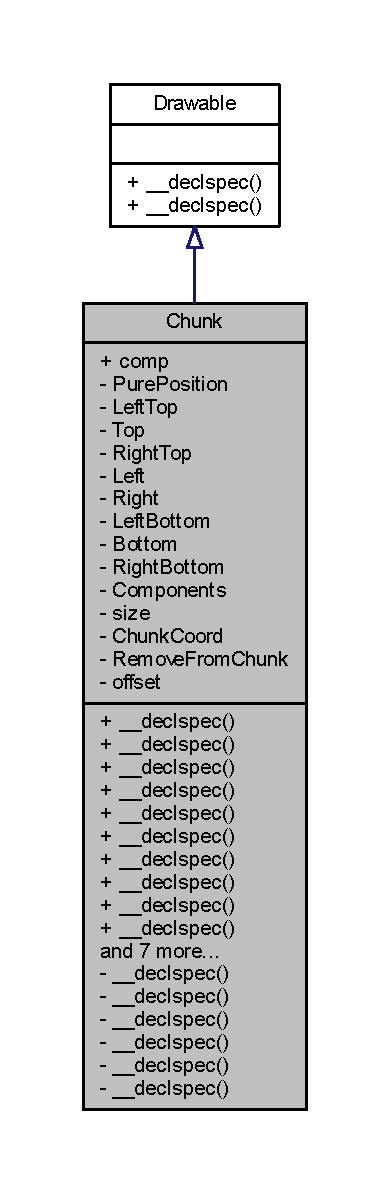
\includegraphics[height=550pt]{class_chunk__inherit__graph}
\end{center}
\end{figure}


Collaboration diagram for Chunk\-:
\nopagebreak
\begin{figure}[H]
\begin{center}
\leavevmode
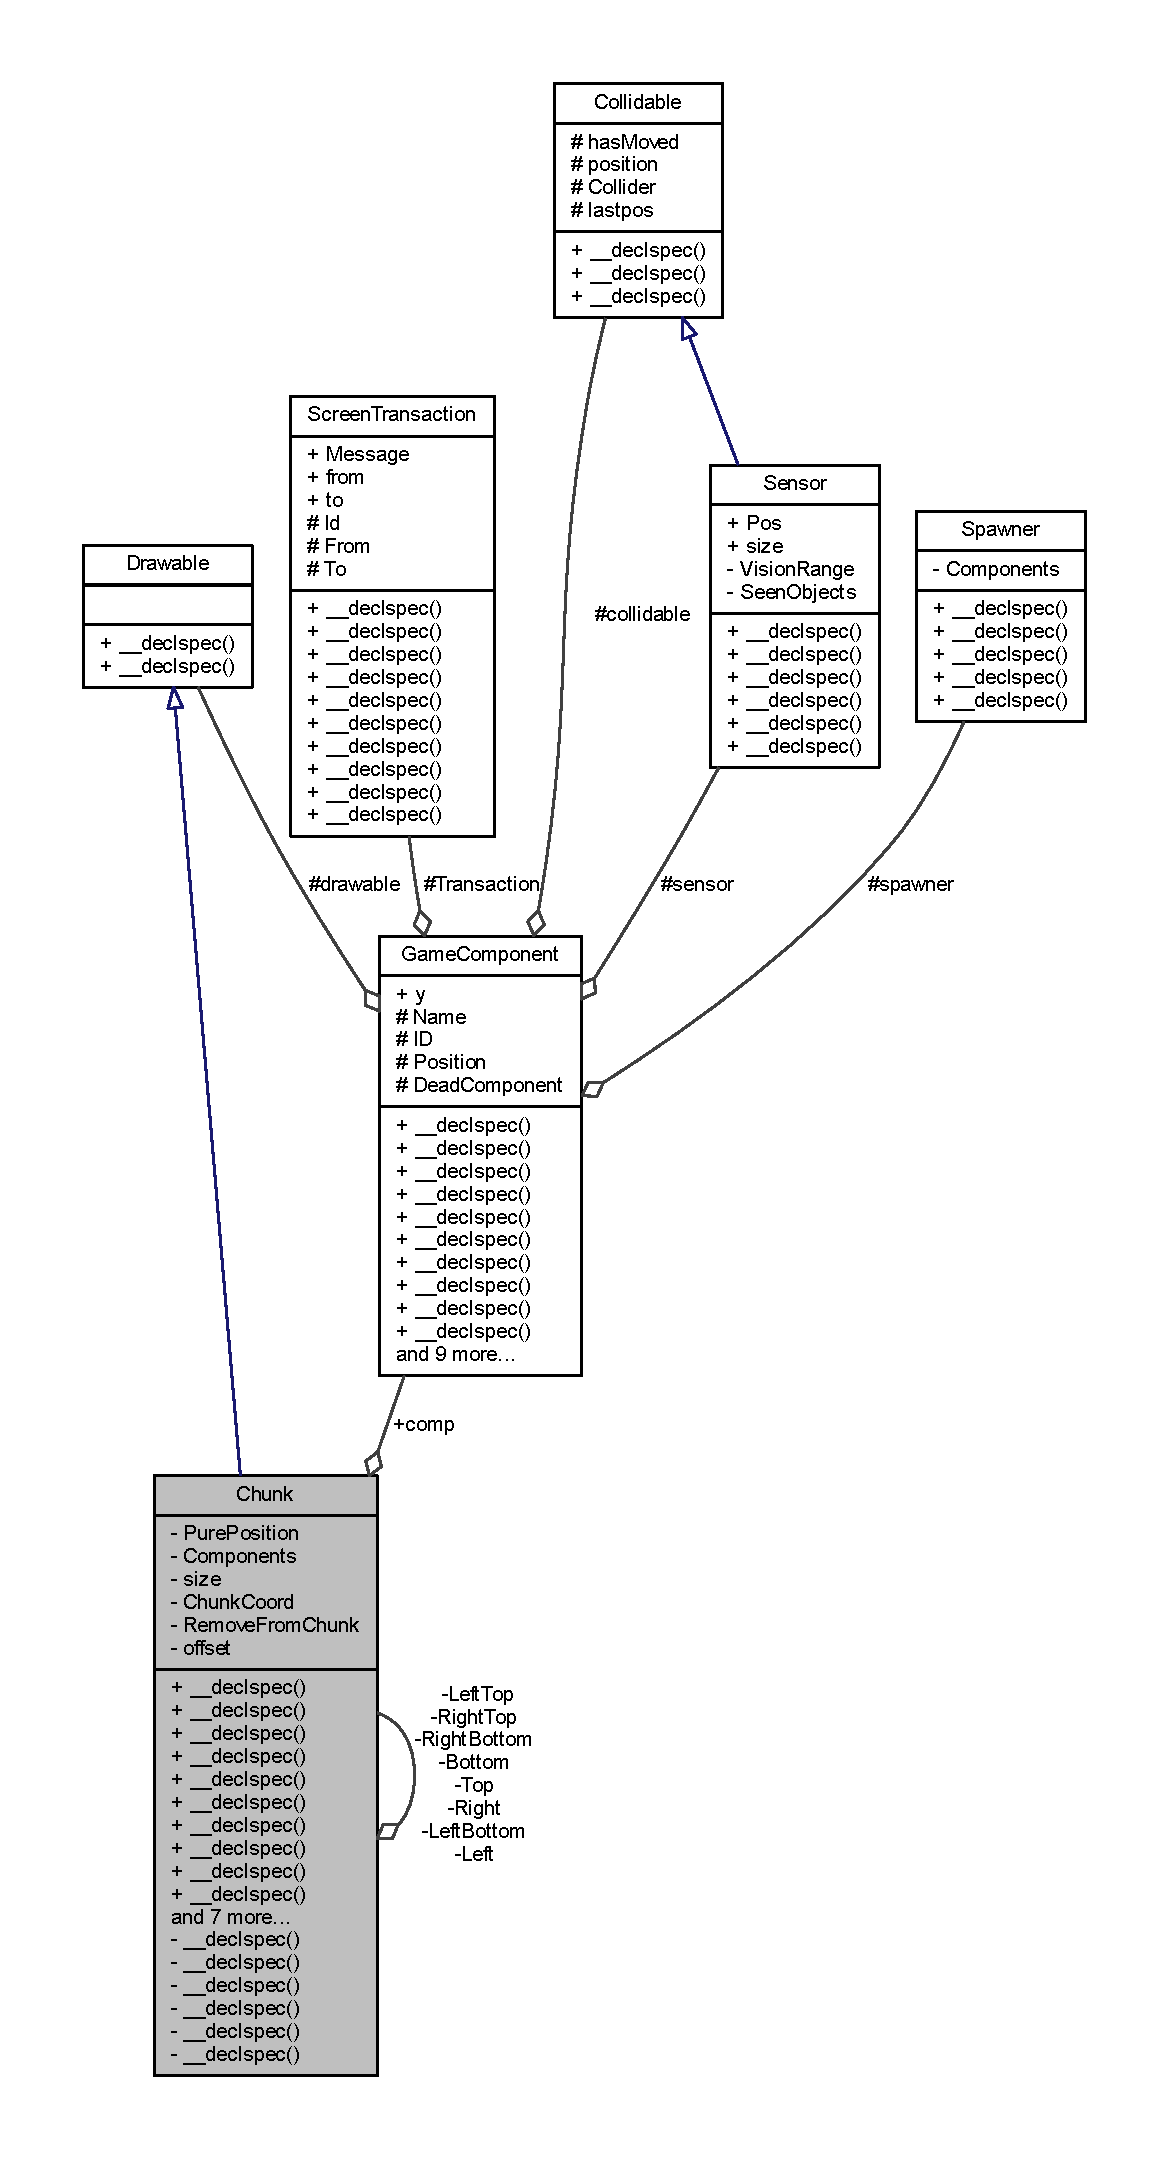
\includegraphics[height=550pt]{class_chunk__coll__graph}
\end{center}
\end{figure}
\subsection*{Public Member Functions}
\begin{DoxyCompactItemize}
\item 
\-\_\-\-\_\-declspec(dllexport) \hyperlink{class_chunk}{Chunk}(sf \hyperlink{class_chunk_ab44ec5e17f0ca6096892265ebf4a448d}{\-\_\-\-\_\-declspec} (dllexport)$\sim$\hyperlink{class_chunk}{Chunk}()
\begin{DoxyCompactList}\small\item\em The constructor. \end{DoxyCompactList}\item 
\hyperlink{class_chunk_ac74827ffc5c989b29d5ee985e0df4e96}{\-\_\-\-\_\-declspec} (dllexport) void add\-Component(\hyperlink{class_game_component}{Game\-Component} $\ast$component)
\begin{DoxyCompactList}\small\item\em This method adds a gamecomponent to the chunk or pushes it to the next if it is out of bounds. \end{DoxyCompactList}\item 
\hyperlink{class_chunk_acb635e1e8318e7b3a0accd4bcf49866d}{\-\_\-\-\_\-declspec} (dllexport) void Update(const \hyperlink{class_update_data}{Update\-Data} \&updateobject)
\begin{DoxyCompactList}\small\item\em This method pushes the update signal to all its components. \end{DoxyCompactList}\item 
\hyperlink{class_chunk_a27a4e5721687f011d6c52624d01eca8d}{\-\_\-\-\_\-declspec} (dllexport) void set\-Top(\hyperlink{class_chunk}{Chunk} $\ast$top)
\begin{DoxyCompactList}\small\item\em This method sets a chunk as the chunk to the top. \end{DoxyCompactList}\item 
\hyperlink{class_chunk_a164b8ab3a4d2e88b6d1bc5e6edfef100}{\-\_\-\-\_\-declspec} (dllexport) void set\-Right\-Top(\hyperlink{class_chunk}{Chunk} $\ast$righttop)
\begin{DoxyCompactList}\small\item\em This method sets a chunk as the chunk to the top right. \end{DoxyCompactList}\item 
\hyperlink{class_chunk_a5e25de330ba7c7c2e557a823d7a8505b}{\-\_\-\-\_\-declspec} (dllexport) void set\-Left(\hyperlink{class_chunk}{Chunk} $\ast$left)
\begin{DoxyCompactList}\small\item\em This method sets a chunk as the chunk to the left. \end{DoxyCompactList}\item 
\hyperlink{class_chunk_ac390d85879176e6e8a26667ba97f8eee}{\-\_\-\-\_\-declspec} (dllexport) void set\-Right(\hyperlink{class_chunk}{Chunk} $\ast$right)
\begin{DoxyCompactList}\small\item\em This method sets a chunk as the chunk to the right. \end{DoxyCompactList}\item 
\hyperlink{class_chunk_a5f6e70225dcd2d5f2cf0c3f77abdfa4b}{\-\_\-\-\_\-declspec} (dllexport) void set\-Left\-Bottom(\hyperlink{class_chunk}{Chunk} $\ast$leftbottom)
\begin{DoxyCompactList}\small\item\em This method sets a chunk as the chunk to the bottom left. \end{DoxyCompactList}\item 
\hyperlink{class_chunk_a69ed23533460c9308dc6ae6e92143e65}{\-\_\-\-\_\-declspec} (dllexport) void set\-Bottom(\hyperlink{class_chunk}{Chunk} $\ast$bottom)
\begin{DoxyCompactList}\small\item\em This method sets a chunk as the chunk to the bottom. \end{DoxyCompactList}\item 
\hyperlink{class_chunk_a42b5a5cf3a22b7cdd14e5e16f9c74ed0}{\-\_\-\-\_\-declspec} (dllexport) void set\-Right\-Bottom(\hyperlink{class_chunk}{Chunk} $\ast$rightbottom)
\begin{DoxyCompactList}\small\item\em This method sets a chunk as the chunk to the bottom right. \end{DoxyCompactList}\item 
\hyperlink{class_chunk_a023a2a543fc48c2b9ba5d2e31eb42e2a}{\-\_\-\-\_\-declspec} (dllexport) \hyperlink{class_chunk}{Chunk} $\ast$get\-Top()
\begin{DoxyCompactList}\small\item\em This method returns the chunk to the top. \end{DoxyCompactList}\item 
\hyperlink{class_chunk_a9b1f0c64473950040eff7ac832ae07f7}{\-\_\-\-\_\-declspec} (dllexport) \hyperlink{class_chunk}{Chunk} $\ast$get\-Left()
\begin{DoxyCompactList}\small\item\em This method returns the chunk to the left. \end{DoxyCompactList}\item 
\hyperlink{class_chunk_a55bd34d914023066cf0bdd1297c3ae8f}{\-\_\-\-\_\-declspec} (dllexport) \hyperlink{class_chunk}{Chunk} $\ast$get\-Right()
\begin{DoxyCompactList}\small\item\em This method returns the chunk to the right. \end{DoxyCompactList}\item 
\hyperlink{class_chunk_a4a65f82eed937ca57e26fbfc8b449fd2}{\-\_\-\-\_\-declspec} (dllexport) \hyperlink{class_chunk}{Chunk} $\ast$get\-Bottom()
\begin{DoxyCompactList}\small\item\em This method returns the chunk to the bottom. \end{DoxyCompactList}\item 
\hyperlink{class_chunk_a11a6eb32b5444ba24bb506e1a57ad4b8}{\-\_\-\-\_\-declspec} (dllexport) sf
\begin{DoxyCompactList}\small\item\em This method returns the chunk coordinates. \end{DoxyCompactList}\item 
\hyperlink{class_chunk_a2a4b74bc2a675752c97407233d14cbaf}{\-\_\-\-\_\-declspec} (dllexport) void Sense\-Single(const \hyperlink{class_update_data}{Update\-Data} \&updateobject
\begin{DoxyCompactList}\small\item\em This method calculates the vision of a single component. \end{DoxyCompactList}\item 
\hyperlink{class_chunk_aabce986183d5f99c1c89a80b51127aa9}{\-\_\-\-\_\-declspec} (dllexport) void Collide\-Single(const \hyperlink{class_update_data}{Update\-Data} \&updateobject
\begin{DoxyCompactList}\small\item\em This method calculates the collision of a single component. \end{DoxyCompactList}\item 
\hyperlink{class_chunk_a11a6eb32b5444ba24bb506e1a57ad4b8}{\-\_\-\-\_\-declspec} (dllexport) sf
\begin{DoxyCompactList}\small\item\em This method returns the real position of the chunk. \end{DoxyCompactList}\item 
\hyperlink{class_chunk_acf3fa4e0c9a7ef9c820c3ba001e449fb}{\-\_\-\-\_\-declspec} (dllexport) float get\-Size()
\begin{DoxyCompactList}\small\item\em This method returns the size of the chunk. \end{DoxyCompactList}\end{DoxyCompactItemize}
\subsection*{Public Attributes}
\begin{DoxyCompactItemize}
\item 
\hyperlink{class_game_component}{Game\-Component} $\ast$ \hyperlink{class_chunk_a633545d862acb016a7081c364126c7b8}{comp}
\end{DoxyCompactItemize}
\subsection*{Private Member Functions}
\begin{DoxyCompactItemize}
\item 
\hyperlink{class_chunk_a09fed540af40e1ad76e8ef2babbfe616}{\-\_\-\-\_\-declspec} (dllexport) void Collide(const \hyperlink{class_update_data}{Update\-Data} \&updateobject)
\begin{DoxyCompactList}\small\item\em This method calls Chunk\-::\-Collide\-Single for every component in the chunk. \end{DoxyCompactList}\item 
\hyperlink{class_chunk_a8a24db04cbc32e330b07d34caa61eeb1}{\-\_\-\-\_\-declspec} (dllexport) void Sense(const \hyperlink{class_update_data}{Update\-Data} \&updateobject)
\begin{DoxyCompactList}\small\item\em This method calls Chunk\-::\-Sense\-Single for every component in the chunk. \end{DoxyCompactList}\item 
\hyperlink{class_chunk_a5c65ce716caab3e2c5bd9193f8e29888}{\-\_\-\-\_\-declspec} (dllexport) void Move\-Component\-To\-Next\-Chunk(\hyperlink{class_game_component}{Game\-Component} $\ast$c)
\begin{DoxyCompactList}\small\item\em This method checks if a component still resides inside the chunk if not it will push it to the next chunk. if no next chunk exsists it will pull the component back into its region. \end{DoxyCompactList}\item 
\hyperlink{class_chunk_aad4ce00be30a71cddc9a17226a992a0f}{\-\_\-\-\_\-declspec} (dllexport) bool Axisis\-In\-Bounds(float axis
\begin{DoxyCompactList}\small\item\em a function to simplify the ifstatements in Chunk\-::\-Move\-Component\-To\-Next\-Chunk \end{DoxyCompactList}\item 
\hyperlink{class_chunk_aecb19003f0e0330920cf7695fbdc5700}{\-\_\-\-\_\-declspec} (dllexport) void Remove\-Flagged\-From\-Chunk()
\begin{DoxyCompactList}\small\item\em removes all the \char`\"{}\-Dead\char`\"{} components from the chunk but does not delete them. \end{DoxyCompactList}\end{DoxyCompactItemize}
\subsection*{Private Attributes}
\begin{DoxyCompactItemize}
\item 
sf\-::\-Vector2f \hyperlink{class_chunk_ace1577872b1189bc7fd88a9b3817ce98}{Pure\-Position}
\begin{DoxyCompactList}\small\item\em Contains the real position of the chunk. \end{DoxyCompactList}\item 
\hyperlink{class_chunk}{Chunk} $\ast$ \hyperlink{class_chunk_a877d51226eaa97c40c05223987514d59}{Left\-Top}
\begin{DoxyCompactList}\small\item\em contains a pointer to the topleft chunk. \end{DoxyCompactList}\item 
\hyperlink{class_chunk}{Chunk} $\ast$ \hyperlink{class_chunk_ae841d5ab24dfa5ef8865cb4fa05d089d}{Top}
\begin{DoxyCompactList}\small\item\em contains a pointer to the top chunk. \end{DoxyCompactList}\item 
\hyperlink{class_chunk}{Chunk} $\ast$ \hyperlink{class_chunk_a8a7593c89d4fe5ed193e68b9ed40016b}{Right\-Top}
\begin{DoxyCompactList}\small\item\em contains a pointer to the topright chunk. \end{DoxyCompactList}\item 
\hyperlink{class_chunk}{Chunk} $\ast$ \hyperlink{class_chunk_aee27c2584364a58dc8811e9ada0695dd}{Left}
\begin{DoxyCompactList}\small\item\em contains a pointer to the left chunk. \end{DoxyCompactList}\item 
\hyperlink{class_chunk}{Chunk} $\ast$ \hyperlink{class_chunk_a0bcf134e2aba0ca49370272c2b3f17a4}{Right}
\begin{DoxyCompactList}\small\item\em contains a pointer to the right chunk. \end{DoxyCompactList}\item 
\hyperlink{class_chunk}{Chunk} $\ast$ \hyperlink{class_chunk_af3577f37139ffeb74181d9ce3c48f5e6}{Left\-Bottom}
\begin{DoxyCompactList}\small\item\em contains a pointer to the bottomleft chunk. \end{DoxyCompactList}\item 
\hyperlink{class_chunk}{Chunk} $\ast$ \hyperlink{class_chunk_ac9ac53a727ae045b6f751ec6a68bcaca}{Bottom}
\begin{DoxyCompactList}\small\item\em contains a pointer to the bottom chunk. \end{DoxyCompactList}\item 
\hyperlink{class_chunk}{Chunk} $\ast$ \hyperlink{class_chunk_afded01a9a67540c9f64dde5776021f4b}{Right\-Bottom}
\begin{DoxyCompactList}\small\item\em contains a pointer to the bottomright chunk. \end{DoxyCompactList}\item 
std\-::list$<$ \hyperlink{class_game_component}{Game\-Component} $\ast$ $>$ \hyperlink{class_chunk_a4cdf6febd96ff99b681e37d548617a38}{Components}
\begin{DoxyCompactList}\small\item\em contains a list of components contained in the chunk. \end{DoxyCompactList}\item 
float \hyperlink{class_chunk_af46410b580baf2985b01044d5c041b2e}{size}
\begin{DoxyCompactList}\small\item\em contains the size of the chunk. \end{DoxyCompactList}\item 
sf\-::\-Vector2i \hyperlink{class_chunk_abb5b1842148b3d7c616065766bfd2b33}{Chunk\-Coord}
\begin{DoxyCompactList}\small\item\em contains the coordinates of the chunk \end{DoxyCompactList}\item 
std\-::list$<$ \hyperlink{class_game_component}{Game\-Component} $\ast$ $>$ \hyperlink{class_chunk_adf6692fdab4518524e217cc0ef09d282}{Remove\-From\-Chunk}
\begin{DoxyCompactList}\small\item\em contains a list of components to remove from the chunk. \end{DoxyCompactList}\item 
float \hyperlink{class_chunk_a6ab7f8f3970c886a62ccc1630bc60a16}{offset}
\end{DoxyCompactItemize}


\subsection{Detailed Description}
This Class represents a small portion of a screen. 

This Class represents a small portion of a screen. it makes sure nothing more is drawn than necessary. It handles its own draw and that of the neigboring chunks. and it holds all components that are at its location. further more it handles the vision and collision of the components in it. \begin{DoxyAuthor}{Author}
Tom Verloop 
\end{DoxyAuthor}
\begin{DoxyVersion}{Version}
1.\-0 
\end{DoxyVersion}
\begin{DoxyDate}{Date}
2014-\/2015 
\end{DoxyDate}
\begin{DoxyRefDesc}{Bug}
\item[\hyperlink{bug__bug000001}{Bug}]anything with a vision greater that one chunk next to it is useless. \end{DoxyRefDesc}


\subsection{Member Function Documentation}
\hypertarget{class_chunk_ab44ec5e17f0ca6096892265ebf4a448d}{\index{Chunk@{Chunk}!\-\_\-\-\_\-declspec@{\-\_\-\-\_\-declspec}}
\index{\-\_\-\-\_\-declspec@{\-\_\-\-\_\-declspec}!Chunk@{Chunk}}
\subsubsection[{\-\_\-\-\_\-declspec}]{\setlength{\rightskip}{0pt plus 5cm}Chunk\-::\-\_\-\-\_\-declspec (
\begin{DoxyParamCaption}
\item[{dllexport}]{}
\end{DoxyParamCaption}
)}}\label{class_chunk_ab44ec5e17f0ca6096892265ebf4a448d}


The constructor. 

This method pushes the Draw\-Self signal to all its neighboring chunks and itself.


\begin{DoxyParams}[1]{Parameters}
\mbox{\tt in}  & {\em Chunk\-Coord} & contains the coordinates used to calculate its real position on the screen. \\
\hline
\mbox{\tt in}  & {\em size} & contains the size of the chunk used to contain its components in.\\
\hline
\end{DoxyParams}
The Deconstructor.


\begin{DoxyParams}[1]{Parameters}
\mbox{\tt in}  & {\em window} & holds an reference to the renderwindow to draw upon. \\
\hline
\mbox{\tt in}  & {\em offset} & holds an position to add to the one of the component.\\
\hline
\end{DoxyParams}
This method pushes the draw signal to all its components. 
\begin{DoxyParams}[1]{Parameters}
\mbox{\tt in}  & {\em window} & holds an reference to the renderwindow to draw upon. \\
\hline
\mbox{\tt in}  & {\em offset} & holds an position to add to the one of the component. \\
\hline
\mbox{\tt in}  & {\em offset} & holds an position from where the draw method was called on the screen.\\
\hline
\end{DoxyParams}
This method sets a chunk as the chunk to the top left. 
\begin{DoxyParams}[1]{Parameters}
\mbox{\tt in}  & {\em lefttop} & contains a pointer to the chunk that should be to the top left. \\
\hline
\end{DoxyParams}
\hypertarget{class_chunk_ac74827ffc5c989b29d5ee985e0df4e96}{\index{Chunk@{Chunk}!\-\_\-\-\_\-declspec@{\-\_\-\-\_\-declspec}}
\index{\-\_\-\-\_\-declspec@{\-\_\-\-\_\-declspec}!Chunk@{Chunk}}
\subsubsection[{\-\_\-\-\_\-declspec}]{\setlength{\rightskip}{0pt plus 5cm}Chunk\-::\-\_\-\-\_\-declspec (
\begin{DoxyParamCaption}
\item[{dllexport}]{}
\end{DoxyParamCaption}
)}}\label{class_chunk_ac74827ffc5c989b29d5ee985e0df4e96}


This method adds a gamecomponent to the chunk or pushes it to the next if it is out of bounds. 


\begin{DoxyParams}[1]{Parameters}
\mbox{\tt in}  & {\em component} & contains a pointer to the component it is supposed to hold. \\
\hline
\end{DoxyParams}
\hypertarget{class_chunk_acb635e1e8318e7b3a0accd4bcf49866d}{\index{Chunk@{Chunk}!\-\_\-\-\_\-declspec@{\-\_\-\-\_\-declspec}}
\index{\-\_\-\-\_\-declspec@{\-\_\-\-\_\-declspec}!Chunk@{Chunk}}
\subsubsection[{\-\_\-\-\_\-declspec}]{\setlength{\rightskip}{0pt plus 5cm}Chunk\-::\-\_\-\-\_\-declspec (
\begin{DoxyParamCaption}
\item[{dllexport}]{}
\end{DoxyParamCaption}
) const}}\label{class_chunk_acb635e1e8318e7b3a0accd4bcf49866d}


This method pushes the update signal to all its components. 


\begin{DoxyParams}[1]{Parameters}
\mbox{\tt in}  & {\em updateobject} & contains a reference to the updateobject containing updatedata. \\
\hline
\end{DoxyParams}
\hypertarget{class_chunk_a27a4e5721687f011d6c52624d01eca8d}{\index{Chunk@{Chunk}!\-\_\-\-\_\-declspec@{\-\_\-\-\_\-declspec}}
\index{\-\_\-\-\_\-declspec@{\-\_\-\-\_\-declspec}!Chunk@{Chunk}}
\subsubsection[{\-\_\-\-\_\-declspec}]{\setlength{\rightskip}{0pt plus 5cm}Chunk\-::\-\_\-\-\_\-declspec (
\begin{DoxyParamCaption}
\item[{dllexport}]{}
\end{DoxyParamCaption}
)}}\label{class_chunk_a27a4e5721687f011d6c52624d01eca8d}


This method sets a chunk as the chunk to the top. 


\begin{DoxyParams}[1]{Parameters}
\mbox{\tt in}  & {\em top} & contains a pointer to the chunk that should be to the top. \\
\hline
\end{DoxyParams}
\hypertarget{class_chunk_a164b8ab3a4d2e88b6d1bc5e6edfef100}{\index{Chunk@{Chunk}!\-\_\-\-\_\-declspec@{\-\_\-\-\_\-declspec}}
\index{\-\_\-\-\_\-declspec@{\-\_\-\-\_\-declspec}!Chunk@{Chunk}}
\subsubsection[{\-\_\-\-\_\-declspec}]{\setlength{\rightskip}{0pt plus 5cm}Chunk\-::\-\_\-\-\_\-declspec (
\begin{DoxyParamCaption}
\item[{dllexport}]{}
\end{DoxyParamCaption}
)}}\label{class_chunk_a164b8ab3a4d2e88b6d1bc5e6edfef100}


This method sets a chunk as the chunk to the top right. 


\begin{DoxyParams}[1]{Parameters}
\mbox{\tt in}  & {\em righttop} & contains a pointer to the chunk that should be to the top right. \\
\hline
\end{DoxyParams}
\hypertarget{class_chunk_a5e25de330ba7c7c2e557a823d7a8505b}{\index{Chunk@{Chunk}!\-\_\-\-\_\-declspec@{\-\_\-\-\_\-declspec}}
\index{\-\_\-\-\_\-declspec@{\-\_\-\-\_\-declspec}!Chunk@{Chunk}}
\subsubsection[{\-\_\-\-\_\-declspec}]{\setlength{\rightskip}{0pt plus 5cm}Chunk\-::\-\_\-\-\_\-declspec (
\begin{DoxyParamCaption}
\item[{dllexport}]{}
\end{DoxyParamCaption}
)}}\label{class_chunk_a5e25de330ba7c7c2e557a823d7a8505b}


This method sets a chunk as the chunk to the left. 


\begin{DoxyParams}[1]{Parameters}
\mbox{\tt in}  & {\em left} & contains a pointer to the chunk that should be to the left. \\
\hline
\end{DoxyParams}
\hypertarget{class_chunk_ac390d85879176e6e8a26667ba97f8eee}{\index{Chunk@{Chunk}!\-\_\-\-\_\-declspec@{\-\_\-\-\_\-declspec}}
\index{\-\_\-\-\_\-declspec@{\-\_\-\-\_\-declspec}!Chunk@{Chunk}}
\subsubsection[{\-\_\-\-\_\-declspec}]{\setlength{\rightskip}{0pt plus 5cm}Chunk\-::\-\_\-\-\_\-declspec (
\begin{DoxyParamCaption}
\item[{dllexport}]{}
\end{DoxyParamCaption}
)}}\label{class_chunk_ac390d85879176e6e8a26667ba97f8eee}


This method sets a chunk as the chunk to the right. 


\begin{DoxyParams}[1]{Parameters}
\mbox{\tt in}  & {\em right} & contains a pointer to the chunk that should be to the right. \\
\hline
\end{DoxyParams}
\hypertarget{class_chunk_a5f6e70225dcd2d5f2cf0c3f77abdfa4b}{\index{Chunk@{Chunk}!\-\_\-\-\_\-declspec@{\-\_\-\-\_\-declspec}}
\index{\-\_\-\-\_\-declspec@{\-\_\-\-\_\-declspec}!Chunk@{Chunk}}
\subsubsection[{\-\_\-\-\_\-declspec}]{\setlength{\rightskip}{0pt plus 5cm}Chunk\-::\-\_\-\-\_\-declspec (
\begin{DoxyParamCaption}
\item[{dllexport}]{}
\end{DoxyParamCaption}
)}}\label{class_chunk_a5f6e70225dcd2d5f2cf0c3f77abdfa4b}


This method sets a chunk as the chunk to the bottom left. 


\begin{DoxyParams}[1]{Parameters}
\mbox{\tt in}  & {\em leftbottom} & contains a pointer to the chunk that should be to the bottom left. \\
\hline
\end{DoxyParams}
\hypertarget{class_chunk_a69ed23533460c9308dc6ae6e92143e65}{\index{Chunk@{Chunk}!\-\_\-\-\_\-declspec@{\-\_\-\-\_\-declspec}}
\index{\-\_\-\-\_\-declspec@{\-\_\-\-\_\-declspec}!Chunk@{Chunk}}
\subsubsection[{\-\_\-\-\_\-declspec}]{\setlength{\rightskip}{0pt plus 5cm}Chunk\-::\-\_\-\-\_\-declspec (
\begin{DoxyParamCaption}
\item[{dllexport}]{}
\end{DoxyParamCaption}
)}}\label{class_chunk_a69ed23533460c9308dc6ae6e92143e65}


This method sets a chunk as the chunk to the bottom. 


\begin{DoxyParams}[1]{Parameters}
\mbox{\tt in}  & {\em bottom} & contains a pointer to the chunk that should be to the bottom. \\
\hline
\end{DoxyParams}
\hypertarget{class_chunk_a42b5a5cf3a22b7cdd14e5e16f9c74ed0}{\index{Chunk@{Chunk}!\-\_\-\-\_\-declspec@{\-\_\-\-\_\-declspec}}
\index{\-\_\-\-\_\-declspec@{\-\_\-\-\_\-declspec}!Chunk@{Chunk}}
\subsubsection[{\-\_\-\-\_\-declspec}]{\setlength{\rightskip}{0pt plus 5cm}Chunk\-::\-\_\-\-\_\-declspec (
\begin{DoxyParamCaption}
\item[{dllexport}]{}
\end{DoxyParamCaption}
)}}\label{class_chunk_a42b5a5cf3a22b7cdd14e5e16f9c74ed0}


This method sets a chunk as the chunk to the bottom right. 


\begin{DoxyParams}[1]{Parameters}
\mbox{\tt in}  & {\em rightbottom} & contains a pointer to the chunk that should be to the bottom right. \\
\hline
\end{DoxyParams}
\hypertarget{class_chunk_a023a2a543fc48c2b9ba5d2e31eb42e2a}{\index{Chunk@{Chunk}!\-\_\-\-\_\-declspec@{\-\_\-\-\_\-declspec}}
\index{\-\_\-\-\_\-declspec@{\-\_\-\-\_\-declspec}!Chunk@{Chunk}}
\subsubsection[{\-\_\-\-\_\-declspec}]{\setlength{\rightskip}{0pt plus 5cm}Chunk\-::\-\_\-\-\_\-declspec (
\begin{DoxyParamCaption}
\item[{dllexport}]{}
\end{DoxyParamCaption}
)}}\label{class_chunk_a023a2a543fc48c2b9ba5d2e31eb42e2a}


This method returns the chunk to the top. 

\begin{DoxyReturn}{Returns}
A pointer of the chunk to the top. 
\end{DoxyReturn}
\hypertarget{class_chunk_a9b1f0c64473950040eff7ac832ae07f7}{\index{Chunk@{Chunk}!\-\_\-\-\_\-declspec@{\-\_\-\-\_\-declspec}}
\index{\-\_\-\-\_\-declspec@{\-\_\-\-\_\-declspec}!Chunk@{Chunk}}
\subsubsection[{\-\_\-\-\_\-declspec}]{\setlength{\rightskip}{0pt plus 5cm}Chunk\-::\-\_\-\-\_\-declspec (
\begin{DoxyParamCaption}
\item[{dllexport}]{}
\end{DoxyParamCaption}
)}}\label{class_chunk_a9b1f0c64473950040eff7ac832ae07f7}


This method returns the chunk to the left. 

\begin{DoxyReturn}{Returns}
A pointer of the chunk to the left. 
\end{DoxyReturn}
\hypertarget{class_chunk_a55bd34d914023066cf0bdd1297c3ae8f}{\index{Chunk@{Chunk}!\-\_\-\-\_\-declspec@{\-\_\-\-\_\-declspec}}
\index{\-\_\-\-\_\-declspec@{\-\_\-\-\_\-declspec}!Chunk@{Chunk}}
\subsubsection[{\-\_\-\-\_\-declspec}]{\setlength{\rightskip}{0pt plus 5cm}Chunk\-::\-\_\-\-\_\-declspec (
\begin{DoxyParamCaption}
\item[{dllexport}]{}
\end{DoxyParamCaption}
)}}\label{class_chunk_a55bd34d914023066cf0bdd1297c3ae8f}


This method returns the chunk to the right. 

\begin{DoxyReturn}{Returns}
A pointer of the chunk to the right. 
\end{DoxyReturn}
\hypertarget{class_chunk_a4a65f82eed937ca57e26fbfc8b449fd2}{\index{Chunk@{Chunk}!\-\_\-\-\_\-declspec@{\-\_\-\-\_\-declspec}}
\index{\-\_\-\-\_\-declspec@{\-\_\-\-\_\-declspec}!Chunk@{Chunk}}
\subsubsection[{\-\_\-\-\_\-declspec}]{\setlength{\rightskip}{0pt plus 5cm}Chunk\-::\-\_\-\-\_\-declspec (
\begin{DoxyParamCaption}
\item[{dllexport}]{}
\end{DoxyParamCaption}
)}}\label{class_chunk_a4a65f82eed937ca57e26fbfc8b449fd2}


This method returns the chunk to the bottom. 

\begin{DoxyReturn}{Returns}
A pointer of the chunk to the bottom. 
\end{DoxyReturn}
\hypertarget{class_chunk_a11a6eb32b5444ba24bb506e1a57ad4b8}{\index{Chunk@{Chunk}!\-\_\-\-\_\-declspec@{\-\_\-\-\_\-declspec}}
\index{\-\_\-\-\_\-declspec@{\-\_\-\-\_\-declspec}!Chunk@{Chunk}}
\subsubsection[{\-\_\-\-\_\-declspec}]{\setlength{\rightskip}{0pt plus 5cm}Chunk\-::\-\_\-\-\_\-declspec (
\begin{DoxyParamCaption}
\item[{dllexport}]{}
\end{DoxyParamCaption}
)\hspace{0.3cm}{\ttfamily [inline]}}}\label{class_chunk_a11a6eb32b5444ba24bb506e1a57ad4b8}


This method returns the chunk coordinates. 

\begin{DoxyReturn}{Returns}
A 2d integer vector. 
\end{DoxyReturn}
\hypertarget{class_chunk_a2a4b74bc2a675752c97407233d14cbaf}{\index{Chunk@{Chunk}!\-\_\-\-\_\-declspec@{\-\_\-\-\_\-declspec}}
\index{\-\_\-\-\_\-declspec@{\-\_\-\-\_\-declspec}!Chunk@{Chunk}}
\subsubsection[{\-\_\-\-\_\-declspec}]{\setlength{\rightskip}{0pt plus 5cm}Chunk\-::\-\_\-\-\_\-declspec (
\begin{DoxyParamCaption}
\item[{dllexport}]{}
\end{DoxyParamCaption}
) const}}\label{class_chunk_a2a4b74bc2a675752c97407233d14cbaf}


This method calculates the vision of a single component. 


\begin{DoxyParams}[1]{Parameters}
\mbox{\tt in}  & {\em updateobject} & Contains all data required for the update event. \\
\hline
\mbox{\tt out}  & {\em comp} & Contains the game component who is sensing for other components. \\
\hline
\end{DoxyParams}
\hypertarget{class_chunk_aabce986183d5f99c1c89a80b51127aa9}{\index{Chunk@{Chunk}!\-\_\-\-\_\-declspec@{\-\_\-\-\_\-declspec}}
\index{\-\_\-\-\_\-declspec@{\-\_\-\-\_\-declspec}!Chunk@{Chunk}}
\subsubsection[{\-\_\-\-\_\-declspec}]{\setlength{\rightskip}{0pt plus 5cm}Chunk\-::\-\_\-\-\_\-declspec (
\begin{DoxyParamCaption}
\item[{dllexport}]{}
\end{DoxyParamCaption}
) const}}\label{class_chunk_aabce986183d5f99c1c89a80b51127aa9}


This method calculates the collision of a single component. 


\begin{DoxyParams}[1]{Parameters}
\mbox{\tt in}  & {\em updateobject} & Contains all data required for the update event. \\
\hline
\mbox{\tt out}  & {\em comp} & Contains the game component who is colliding with other components. \\
\hline
\end{DoxyParams}
\hypertarget{class_chunk_a11a6eb32b5444ba24bb506e1a57ad4b8}{\index{Chunk@{Chunk}!\-\_\-\-\_\-declspec@{\-\_\-\-\_\-declspec}}
\index{\-\_\-\-\_\-declspec@{\-\_\-\-\_\-declspec}!Chunk@{Chunk}}
\subsubsection[{\-\_\-\-\_\-declspec}]{\setlength{\rightskip}{0pt plus 5cm}Chunk\-::\-\_\-\-\_\-declspec (
\begin{DoxyParamCaption}
\item[{dllexport}]{}
\end{DoxyParamCaption}
)\hspace{0.3cm}{\ttfamily [inline]}}}\label{class_chunk_a11a6eb32b5444ba24bb506e1a57ad4b8}


This method returns the real position of the chunk. 

\begin{DoxyReturn}{Returns}
A 2\-D float vector containing the position of the chunk. 
\end{DoxyReturn}
\hypertarget{class_chunk_acf3fa4e0c9a7ef9c820c3ba001e449fb}{\index{Chunk@{Chunk}!\-\_\-\-\_\-declspec@{\-\_\-\-\_\-declspec}}
\index{\-\_\-\-\_\-declspec@{\-\_\-\-\_\-declspec}!Chunk@{Chunk}}
\subsubsection[{\-\_\-\-\_\-declspec}]{\setlength{\rightskip}{0pt plus 5cm}Chunk\-::\-\_\-\-\_\-declspec (
\begin{DoxyParamCaption}
\item[{dllexport}]{}
\end{DoxyParamCaption}
)\hspace{0.3cm}{\ttfamily [inline]}}}\label{class_chunk_acf3fa4e0c9a7ef9c820c3ba001e449fb}


This method returns the size of the chunk. 

\begin{DoxyReturn}{Returns}
A float containing the size of the chunk. 
\end{DoxyReturn}
\hypertarget{class_chunk_a09fed540af40e1ad76e8ef2babbfe616}{\index{Chunk@{Chunk}!\-\_\-\-\_\-declspec@{\-\_\-\-\_\-declspec}}
\index{\-\_\-\-\_\-declspec@{\-\_\-\-\_\-declspec}!Chunk@{Chunk}}
\subsubsection[{\-\_\-\-\_\-declspec}]{\setlength{\rightskip}{0pt plus 5cm}Chunk\-::\-\_\-\-\_\-declspec (
\begin{DoxyParamCaption}
\item[{dllexport}]{}
\end{DoxyParamCaption}
) const\hspace{0.3cm}{\ttfamily [private]}}}\label{class_chunk_a09fed540af40e1ad76e8ef2babbfe616}


This method calls Chunk\-::\-Collide\-Single for every component in the chunk. 


\begin{DoxyParams}[1]{Parameters}
\mbox{\tt in}  & {\em updateobject} & contains all data for the update event. \\
\hline
\end{DoxyParams}
\hypertarget{class_chunk_a8a24db04cbc32e330b07d34caa61eeb1}{\index{Chunk@{Chunk}!\-\_\-\-\_\-declspec@{\-\_\-\-\_\-declspec}}
\index{\-\_\-\-\_\-declspec@{\-\_\-\-\_\-declspec}!Chunk@{Chunk}}
\subsubsection[{\-\_\-\-\_\-declspec}]{\setlength{\rightskip}{0pt plus 5cm}Chunk\-::\-\_\-\-\_\-declspec (
\begin{DoxyParamCaption}
\item[{dllexport}]{}
\end{DoxyParamCaption}
) const\hspace{0.3cm}{\ttfamily [private]}}}\label{class_chunk_a8a24db04cbc32e330b07d34caa61eeb1}


This method calls Chunk\-::\-Sense\-Single for every component in the chunk. 


\begin{DoxyParams}[1]{Parameters}
\mbox{\tt in}  & {\em updateobject} & contains all data for the update event. \\
\hline
\end{DoxyParams}
\hypertarget{class_chunk_a5c65ce716caab3e2c5bd9193f8e29888}{\index{Chunk@{Chunk}!\-\_\-\-\_\-declspec@{\-\_\-\-\_\-declspec}}
\index{\-\_\-\-\_\-declspec@{\-\_\-\-\_\-declspec}!Chunk@{Chunk}}
\subsubsection[{\-\_\-\-\_\-declspec}]{\setlength{\rightskip}{0pt plus 5cm}Chunk\-::\-\_\-\-\_\-declspec (
\begin{DoxyParamCaption}
\item[{dllexport}]{}
\end{DoxyParamCaption}
)\hspace{0.3cm}{\ttfamily [private]}}}\label{class_chunk_a5c65ce716caab3e2c5bd9193f8e29888}


This method checks if a component still resides inside the chunk if not it will push it to the next chunk. if no next chunk exsists it will pull the component back into its region. 


\begin{DoxyParams}[1]{Parameters}
\mbox{\tt in}  & {\em c} & Contains the component to check. \\
\hline
\end{DoxyParams}
\hypertarget{class_chunk_aad4ce00be30a71cddc9a17226a992a0f}{\index{Chunk@{Chunk}!\-\_\-\-\_\-declspec@{\-\_\-\-\_\-declspec}}
\index{\-\_\-\-\_\-declspec@{\-\_\-\-\_\-declspec}!Chunk@{Chunk}}
\subsubsection[{\-\_\-\-\_\-declspec}]{\setlength{\rightskip}{0pt plus 5cm}Chunk\-::\-\_\-\-\_\-declspec (
\begin{DoxyParamCaption}
\item[{dllexport}]{}
\end{DoxyParamCaption}
)\hspace{0.3cm}{\ttfamily [private]}}}\label{class_chunk_aad4ce00be30a71cddc9a17226a992a0f}


a function to simplify the ifstatements in Chunk\-::\-Move\-Component\-To\-Next\-Chunk 


\begin{DoxyParams}[1]{Parameters}
\mbox{\tt in}  & {\em axis} & Contains the axis to check on. \\
\hline
\mbox{\tt in}  & {\em offset} & Contains the offset to check on. \\
\hline
\end{DoxyParams}
\begin{DoxyReturn}{Returns}
Returns true if the axis is in bounds. 
\end{DoxyReturn}
\hypertarget{class_chunk_aecb19003f0e0330920cf7695fbdc5700}{\index{Chunk@{Chunk}!\-\_\-\-\_\-declspec@{\-\_\-\-\_\-declspec}}
\index{\-\_\-\-\_\-declspec@{\-\_\-\-\_\-declspec}!Chunk@{Chunk}}
\subsubsection[{\-\_\-\-\_\-declspec}]{\setlength{\rightskip}{0pt plus 5cm}Chunk\-::\-\_\-\-\_\-declspec (
\begin{DoxyParamCaption}
\item[{dllexport}]{}
\end{DoxyParamCaption}
)\hspace{0.3cm}{\ttfamily [private]}}}\label{class_chunk_aecb19003f0e0330920cf7695fbdc5700}


removes all the \char`\"{}\-Dead\char`\"{} components from the chunk but does not delete them. 



\subsection{Member Data Documentation}
\hypertarget{class_chunk_ac9ac53a727ae045b6f751ec6a68bcaca}{\index{Chunk@{Chunk}!Bottom@{Bottom}}
\index{Bottom@{Bottom}!Chunk@{Chunk}}
\subsubsection[{Bottom}]{\setlength{\rightskip}{0pt plus 5cm}{\bf Chunk}$\ast$ Chunk\-::\-Bottom\hspace{0.3cm}{\ttfamily [private]}}}\label{class_chunk_ac9ac53a727ae045b6f751ec6a68bcaca}


contains a pointer to the bottom chunk. 

\hypertarget{class_chunk_abb5b1842148b3d7c616065766bfd2b33}{\index{Chunk@{Chunk}!Chunk\-Coord@{Chunk\-Coord}}
\index{Chunk\-Coord@{Chunk\-Coord}!Chunk@{Chunk}}
\subsubsection[{Chunk\-Coord}]{\setlength{\rightskip}{0pt plus 5cm}sf\-::\-Vector2i Chunk\-::\-Chunk\-Coord\hspace{0.3cm}{\ttfamily [private]}}}\label{class_chunk_abb5b1842148b3d7c616065766bfd2b33}


contains the coordinates of the chunk 

\hypertarget{class_chunk_a633545d862acb016a7081c364126c7b8}{\index{Chunk@{Chunk}!comp@{comp}}
\index{comp@{comp}!Chunk@{Chunk}}
\subsubsection[{comp}]{\setlength{\rightskip}{0pt plus 5cm}{\bf Game\-Component} $\ast$ Chunk\-::comp}}\label{class_chunk_a633545d862acb016a7081c364126c7b8}
\hypertarget{class_chunk_a4cdf6febd96ff99b681e37d548617a38}{\index{Chunk@{Chunk}!Components@{Components}}
\index{Components@{Components}!Chunk@{Chunk}}
\subsubsection[{Components}]{\setlength{\rightskip}{0pt plus 5cm}std\-::list$<${\bf Game\-Component}$\ast$$>$ Chunk\-::\-Components\hspace{0.3cm}{\ttfamily [private]}}}\label{class_chunk_a4cdf6febd96ff99b681e37d548617a38}


contains a list of components contained in the chunk. 

\hypertarget{class_chunk_aee27c2584364a58dc8811e9ada0695dd}{\index{Chunk@{Chunk}!Left@{Left}}
\index{Left@{Left}!Chunk@{Chunk}}
\subsubsection[{Left}]{\setlength{\rightskip}{0pt plus 5cm}{\bf Chunk}$\ast$ Chunk\-::\-Left\hspace{0.3cm}{\ttfamily [private]}}}\label{class_chunk_aee27c2584364a58dc8811e9ada0695dd}


contains a pointer to the left chunk. 

\hypertarget{class_chunk_af3577f37139ffeb74181d9ce3c48f5e6}{\index{Chunk@{Chunk}!Left\-Bottom@{Left\-Bottom}}
\index{Left\-Bottom@{Left\-Bottom}!Chunk@{Chunk}}
\subsubsection[{Left\-Bottom}]{\setlength{\rightskip}{0pt plus 5cm}{\bf Chunk}$\ast$ Chunk\-::\-Left\-Bottom\hspace{0.3cm}{\ttfamily [private]}}}\label{class_chunk_af3577f37139ffeb74181d9ce3c48f5e6}


contains a pointer to the bottomleft chunk. 

\hypertarget{class_chunk_a877d51226eaa97c40c05223987514d59}{\index{Chunk@{Chunk}!Left\-Top@{Left\-Top}}
\index{Left\-Top@{Left\-Top}!Chunk@{Chunk}}
\subsubsection[{Left\-Top}]{\setlength{\rightskip}{0pt plus 5cm}{\bf Chunk}$\ast$ Chunk\-::\-Left\-Top\hspace{0.3cm}{\ttfamily [private]}}}\label{class_chunk_a877d51226eaa97c40c05223987514d59}


contains a pointer to the topleft chunk. 

\hypertarget{class_chunk_a6ab7f8f3970c886a62ccc1630bc60a16}{\index{Chunk@{Chunk}!offset@{offset}}
\index{offset@{offset}!Chunk@{Chunk}}
\subsubsection[{offset}]{\setlength{\rightskip}{0pt plus 5cm}float Chunk\-::offset\hspace{0.3cm}{\ttfamily [private]}}}\label{class_chunk_a6ab7f8f3970c886a62ccc1630bc60a16}
\hypertarget{class_chunk_ace1577872b1189bc7fd88a9b3817ce98}{\index{Chunk@{Chunk}!Pure\-Position@{Pure\-Position}}
\index{Pure\-Position@{Pure\-Position}!Chunk@{Chunk}}
\subsubsection[{Pure\-Position}]{\setlength{\rightskip}{0pt plus 5cm}sf\-::\-Vector2f Chunk\-::\-Pure\-Position\hspace{0.3cm}{\ttfamily [private]}}}\label{class_chunk_ace1577872b1189bc7fd88a9b3817ce98}


Contains the real position of the chunk. 

\hypertarget{class_chunk_adf6692fdab4518524e217cc0ef09d282}{\index{Chunk@{Chunk}!Remove\-From\-Chunk@{Remove\-From\-Chunk}}
\index{Remove\-From\-Chunk@{Remove\-From\-Chunk}!Chunk@{Chunk}}
\subsubsection[{Remove\-From\-Chunk}]{\setlength{\rightskip}{0pt plus 5cm}std\-::list$<${\bf Game\-Component}$\ast$$>$ Chunk\-::\-Remove\-From\-Chunk\hspace{0.3cm}{\ttfamily [private]}}}\label{class_chunk_adf6692fdab4518524e217cc0ef09d282}


contains a list of components to remove from the chunk. 

\hypertarget{class_chunk_a0bcf134e2aba0ca49370272c2b3f17a4}{\index{Chunk@{Chunk}!Right@{Right}}
\index{Right@{Right}!Chunk@{Chunk}}
\subsubsection[{Right}]{\setlength{\rightskip}{0pt plus 5cm}{\bf Chunk}$\ast$ Chunk\-::\-Right\hspace{0.3cm}{\ttfamily [private]}}}\label{class_chunk_a0bcf134e2aba0ca49370272c2b3f17a4}


contains a pointer to the right chunk. 

\hypertarget{class_chunk_afded01a9a67540c9f64dde5776021f4b}{\index{Chunk@{Chunk}!Right\-Bottom@{Right\-Bottom}}
\index{Right\-Bottom@{Right\-Bottom}!Chunk@{Chunk}}
\subsubsection[{Right\-Bottom}]{\setlength{\rightskip}{0pt plus 5cm}{\bf Chunk}$\ast$ Chunk\-::\-Right\-Bottom\hspace{0.3cm}{\ttfamily [private]}}}\label{class_chunk_afded01a9a67540c9f64dde5776021f4b}


contains a pointer to the bottomright chunk. 

\hypertarget{class_chunk_a8a7593c89d4fe5ed193e68b9ed40016b}{\index{Chunk@{Chunk}!Right\-Top@{Right\-Top}}
\index{Right\-Top@{Right\-Top}!Chunk@{Chunk}}
\subsubsection[{Right\-Top}]{\setlength{\rightskip}{0pt plus 5cm}{\bf Chunk}$\ast$ Chunk\-::\-Right\-Top\hspace{0.3cm}{\ttfamily [private]}}}\label{class_chunk_a8a7593c89d4fe5ed193e68b9ed40016b}


contains a pointer to the topright chunk. 

\hypertarget{class_chunk_af46410b580baf2985b01044d5c041b2e}{\index{Chunk@{Chunk}!size@{size}}
\index{size@{size}!Chunk@{Chunk}}
\subsubsection[{size}]{\setlength{\rightskip}{0pt plus 5cm}float Chunk\-::size\hspace{0.3cm}{\ttfamily [private]}}}\label{class_chunk_af46410b580baf2985b01044d5c041b2e}


contains the size of the chunk. 

\hypertarget{class_chunk_ae841d5ab24dfa5ef8865cb4fa05d089d}{\index{Chunk@{Chunk}!Top@{Top}}
\index{Top@{Top}!Chunk@{Chunk}}
\subsubsection[{Top}]{\setlength{\rightskip}{0pt plus 5cm}{\bf Chunk}$\ast$ Chunk\-::\-Top\hspace{0.3cm}{\ttfamily [private]}}}\label{class_chunk_ae841d5ab24dfa5ef8865cb4fa05d089d}


contains a pointer to the top chunk. 



The documentation for this class was generated from the following file\-:\begin{DoxyCompactItemize}
\item 
D\-:/\-Users/tom/\-Documents/\-Visual Studio 2013/\-Projects/\-Revelatorframework/\-Revelator\-Framework\-\_\-\-A\-P\-I/\hyperlink{_chunk_8hpp}{Chunk.\-hpp}\end{DoxyCompactItemize}

\hypertarget{class_chunk_manager}{\section{Chunk\-Manager Class Reference}
\label{class_chunk_manager}\index{Chunk\-Manager@{Chunk\-Manager}}
}


{\ttfamily \#include $<$Chunk\-Manager.\-hpp$>$}



Collaboration diagram for Chunk\-Manager\-:
\nopagebreak
\begin{figure}[H]
\begin{center}
\leavevmode
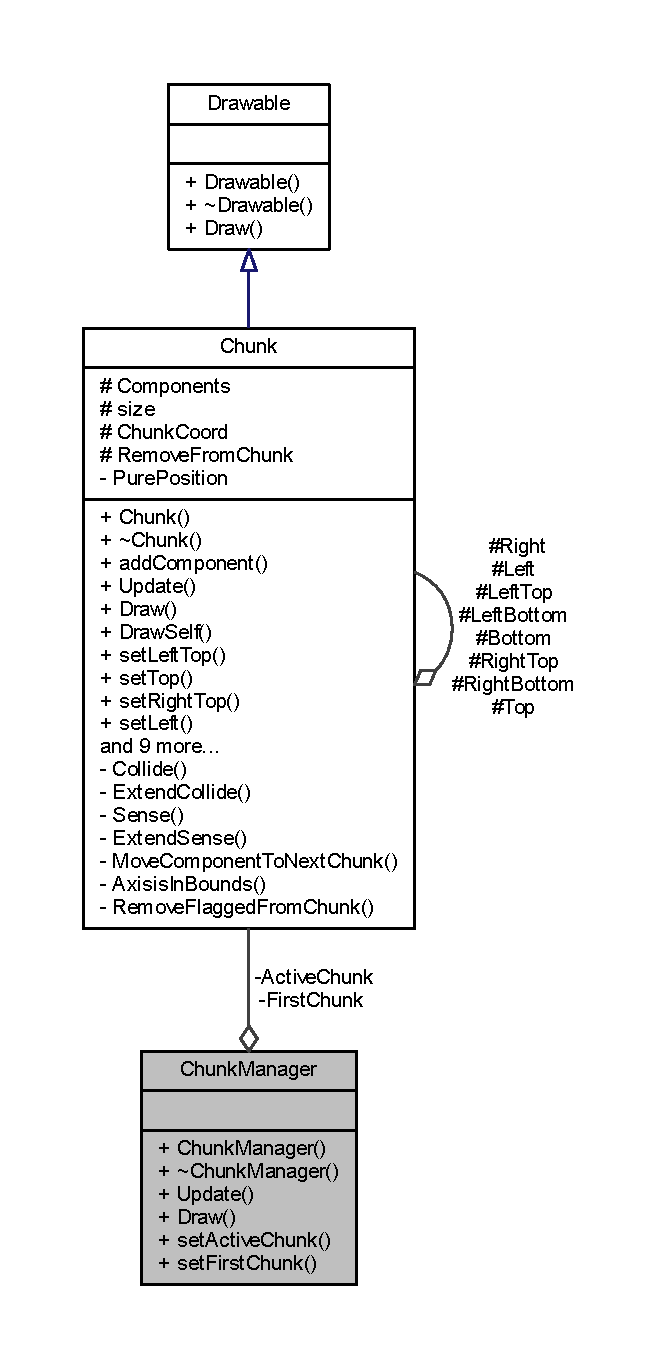
\includegraphics[height=550pt]{class_chunk_manager__coll__graph}
\end{center}
\end{figure}
\subsection*{Public Member Functions}
\begin{DoxyCompactItemize}
\item 
\hyperlink{class_chunk_manager_a5174dca056d736be1e45b71dfc0930ef}{\-\_\-\-\_\-declspec} (dllexport) \hyperlink{class_chunk_manager}{Chunk\-Manager}()
\item 
\hyperlink{class_chunk_manager_a3ea11ca30e6e72f84a1f1bcfe6110543}{\-\_\-\-\_\-declspec} (dllexport)$\sim$\hyperlink{class_chunk_manager}{Chunk\-Manager}()
\item 
\hyperlink{class_chunk_manager_a765c3019448f155961fff4dfeee300ca}{\-\_\-\-\_\-declspec} (dllexport) void Update(const \hyperlink{class_update_data}{Update\-Data} \&updateobject)
\item 
\-\_\-\-\_\-declspec(dllexport) void Draw(sf \hyperlink{class_chunk_manager_a1e77e66b79c2f65848acf922eceebc08}{\-\_\-\-\_\-declspec} (dllexport) void set\-Active\-Chunk(\hyperlink{class_chunk}{Chunk} $\ast$c)
\item 
\hyperlink{class_chunk_manager_aefbc2b592e93d6651226f055eb701d47}{\-\_\-\-\_\-declspec} (dllexport) void set\-First\-Chunk(\hyperlink{class_chunk}{Chunk} $\ast$c)
\item 
\hyperlink{class_chunk_manager_a132a5714695e761d05b32321c721a1d8}{\-\_\-\-\_\-declspec} (dllexport) void add\-Game\-Component(\hyperlink{class_game_component}{Game\-Component} $\ast$c)
\end{DoxyCompactItemize}
\subsection*{Private Attributes}
\begin{DoxyCompactItemize}
\item 
\hyperlink{class_chunk}{Chunk} $\ast$ \hyperlink{class_chunk_manager_a8008f62926fe10f46ac59001aae2d372}{Active\-Chunk}
\item 
\hyperlink{class_chunk}{Chunk} $\ast$ \hyperlink{class_chunk_manager_afb87cd5dd3cb61f09a6038d1796719ba}{First\-Chunk}
\end{DoxyCompactItemize}


\subsection{Member Function Documentation}
\hypertarget{class_chunk_manager_a5174dca056d736be1e45b71dfc0930ef}{\index{Chunk\-Manager@{Chunk\-Manager}!\-\_\-\-\_\-declspec@{\-\_\-\-\_\-declspec}}
\index{\-\_\-\-\_\-declspec@{\-\_\-\-\_\-declspec}!ChunkManager@{Chunk\-Manager}}
\subsubsection[{\-\_\-\-\_\-declspec}]{\setlength{\rightskip}{0pt plus 5cm}Chunk\-Manager\-::\-\_\-\-\_\-declspec (
\begin{DoxyParamCaption}
\item[{dllexport}]{}
\end{DoxyParamCaption}
)}}\label{class_chunk_manager_a5174dca056d736be1e45b71dfc0930ef}
\hypertarget{class_chunk_manager_a3ea11ca30e6e72f84a1f1bcfe6110543}{\index{Chunk\-Manager@{Chunk\-Manager}!\-\_\-\-\_\-declspec@{\-\_\-\-\_\-declspec}}
\index{\-\_\-\-\_\-declspec@{\-\_\-\-\_\-declspec}!ChunkManager@{Chunk\-Manager}}
\subsubsection[{\-\_\-\-\_\-declspec}]{\setlength{\rightskip}{0pt plus 5cm}Chunk\-Manager\-::\-\_\-\-\_\-declspec (
\begin{DoxyParamCaption}
\item[{dllexport}]{}
\end{DoxyParamCaption}
)}}\label{class_chunk_manager_a3ea11ca30e6e72f84a1f1bcfe6110543}
\hypertarget{class_chunk_manager_a765c3019448f155961fff4dfeee300ca}{\index{Chunk\-Manager@{Chunk\-Manager}!\-\_\-\-\_\-declspec@{\-\_\-\-\_\-declspec}}
\index{\-\_\-\-\_\-declspec@{\-\_\-\-\_\-declspec}!ChunkManager@{Chunk\-Manager}}
\subsubsection[{\-\_\-\-\_\-declspec}]{\setlength{\rightskip}{0pt plus 5cm}Chunk\-Manager\-::\-\_\-\-\_\-declspec (
\begin{DoxyParamCaption}
\item[{dllexport}]{}
\end{DoxyParamCaption}
) const}}\label{class_chunk_manager_a765c3019448f155961fff4dfeee300ca}
\hypertarget{class_chunk_manager_a1e77e66b79c2f65848acf922eceebc08}{\index{Chunk\-Manager@{Chunk\-Manager}!\-\_\-\-\_\-declspec@{\-\_\-\-\_\-declspec}}
\index{\-\_\-\-\_\-declspec@{\-\_\-\-\_\-declspec}!ChunkManager@{Chunk\-Manager}}
\subsubsection[{\-\_\-\-\_\-declspec}]{\setlength{\rightskip}{0pt plus 5cm}\-\_\-\-\_\-declspec (dllexport) void Draw(sf Chunk\-Manager\-::\-\_\-\-\_\-declspec (
\begin{DoxyParamCaption}
\item[{dllexport}]{}
\end{DoxyParamCaption}
)}}\label{class_chunk_manager_a1e77e66b79c2f65848acf922eceebc08}
\hypertarget{class_chunk_manager_aefbc2b592e93d6651226f055eb701d47}{\index{Chunk\-Manager@{Chunk\-Manager}!\-\_\-\-\_\-declspec@{\-\_\-\-\_\-declspec}}
\index{\-\_\-\-\_\-declspec@{\-\_\-\-\_\-declspec}!ChunkManager@{Chunk\-Manager}}
\subsubsection[{\-\_\-\-\_\-declspec}]{\setlength{\rightskip}{0pt plus 5cm}Chunk\-Manager\-::\-\_\-\-\_\-declspec (
\begin{DoxyParamCaption}
\item[{dllexport}]{}
\end{DoxyParamCaption}
)}}\label{class_chunk_manager_aefbc2b592e93d6651226f055eb701d47}
\hypertarget{class_chunk_manager_a132a5714695e761d05b32321c721a1d8}{\index{Chunk\-Manager@{Chunk\-Manager}!\-\_\-\-\_\-declspec@{\-\_\-\-\_\-declspec}}
\index{\-\_\-\-\_\-declspec@{\-\_\-\-\_\-declspec}!ChunkManager@{Chunk\-Manager}}
\subsubsection[{\-\_\-\-\_\-declspec}]{\setlength{\rightskip}{0pt plus 5cm}Chunk\-Manager\-::\-\_\-\-\_\-declspec (
\begin{DoxyParamCaption}
\item[{dllexport}]{}
\end{DoxyParamCaption}
)}}\label{class_chunk_manager_a132a5714695e761d05b32321c721a1d8}


\subsection{Member Data Documentation}
\hypertarget{class_chunk_manager_a8008f62926fe10f46ac59001aae2d372}{\index{Chunk\-Manager@{Chunk\-Manager}!Active\-Chunk@{Active\-Chunk}}
\index{Active\-Chunk@{Active\-Chunk}!ChunkManager@{Chunk\-Manager}}
\subsubsection[{Active\-Chunk}]{\setlength{\rightskip}{0pt plus 5cm}{\bf Chunk}$\ast$ Chunk\-Manager\-::\-Active\-Chunk\hspace{0.3cm}{\ttfamily [private]}}}\label{class_chunk_manager_a8008f62926fe10f46ac59001aae2d372}
\hypertarget{class_chunk_manager_afb87cd5dd3cb61f09a6038d1796719ba}{\index{Chunk\-Manager@{Chunk\-Manager}!First\-Chunk@{First\-Chunk}}
\index{First\-Chunk@{First\-Chunk}!ChunkManager@{Chunk\-Manager}}
\subsubsection[{First\-Chunk}]{\setlength{\rightskip}{0pt plus 5cm}{\bf Chunk}$\ast$ Chunk\-Manager\-::\-First\-Chunk\hspace{0.3cm}{\ttfamily [private]}}}\label{class_chunk_manager_afb87cd5dd3cb61f09a6038d1796719ba}


The documentation for this class was generated from the following file\-:\begin{DoxyCompactItemize}
\item 
D\-:/\-Users/tom/\-Documents/\-Visual Studio 2013/\-Projects/\-Revelatorframework/\-Revelator\-Framework\-\_\-\-A\-P\-I/\hyperlink{_chunk_manager_8hpp}{Chunk\-Manager.\-hpp}\end{DoxyCompactItemize}

\hypertarget{class_collidable}{\section{Collidable Class Reference}
\label{class_collidable}\index{Collidable@{Collidable}}
}


{\ttfamily \#include $<$Collidable.\-hpp$>$}



Inheritance diagram for Collidable\-:
\nopagebreak
\begin{figure}[H]
\begin{center}
\leavevmode
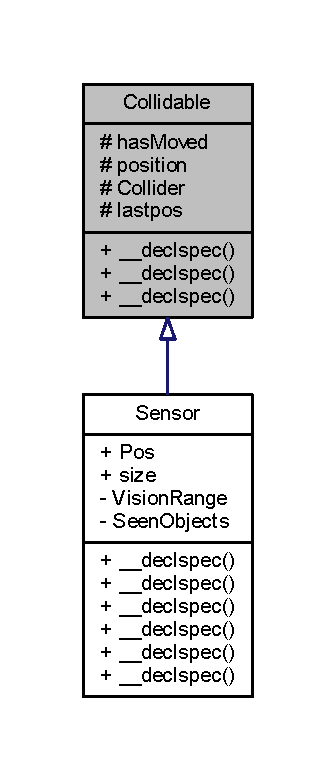
\includegraphics[width=188pt]{class_collidable__inherit__graph}
\end{center}
\end{figure}


Collaboration diagram for Collidable\-:\nopagebreak
\begin{figure}[H]
\begin{center}
\leavevmode
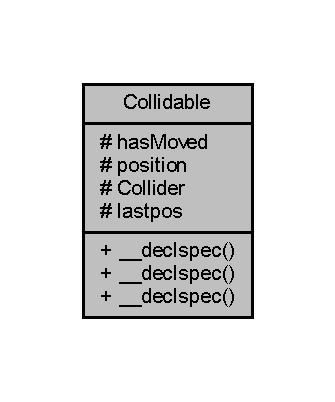
\includegraphics[width=166pt]{class_collidable__coll__graph}
\end{center}
\end{figure}
\subsection*{Public Member Functions}
\begin{DoxyCompactItemize}
\item 
\hyperlink{class_collidable_a92ce9e2b08086bb2f466168ffc69c9ed}{Collidable} ()
\item 
\hyperlink{class_collidable_a71a242ba63c157ca40acbf4421c0eaf7}{Collidable} (sf\-::\-Vector2f $\ast$\hyperlink{class_collidable_aa6c2e113d920df8c0d5da2a244f924bd}{position}, sf\-::\-Vector2f size)
\item 
\hyperlink{class_collidable_a454ca1b66dd504b25fed3706914cee6e}{$\sim$\-Collidable} ()
\item 
\hyperlink{class_rectangle}{Rectangle} \& \hyperlink{class_collidable_ac9edfccd8c5a1ea77238c0a19aa910c3}{get\-Collider} ()
\item 
bool \hyperlink{class_collidable_a8cc1f09ce02e6fcf56d98f07f908a104}{is\-Moved} ()
\end{DoxyCompactItemize}
\subsection*{Protected Attributes}
\begin{DoxyCompactItemize}
\item 
bool \hyperlink{class_collidable_afe5442fd3a82abe62b95e93248d5f4a1}{has\-Moved}
\item 
sf\-::\-Vector2f $\ast$ \hyperlink{class_collidable_aa6c2e113d920df8c0d5da2a244f924bd}{position}
\item 
\hyperlink{class_rectangle}{Rectangle} \hyperlink{class_collidable_a0a81575218d87940935d70800f7d663e}{Collider}
\item 
sf\-::\-Vector2f \hyperlink{class_collidable_ae50dbf8f9d1f584d3a5d5c3445fbe786}{lastpos}
\end{DoxyCompactItemize}


\subsection{Constructor \& Destructor Documentation}
\hypertarget{class_collidable_a92ce9e2b08086bb2f466168ffc69c9ed}{\index{Collidable@{Collidable}!Collidable@{Collidable}}
\index{Collidable@{Collidable}!Collidable@{Collidable}}
\subsubsection[{Collidable}]{\setlength{\rightskip}{0pt plus 5cm}Collidable\-::\-Collidable (
\begin{DoxyParamCaption}
{}
\end{DoxyParamCaption}
)}}\label{class_collidable_a92ce9e2b08086bb2f466168ffc69c9ed}
\hypertarget{class_collidable_a71a242ba63c157ca40acbf4421c0eaf7}{\index{Collidable@{Collidable}!Collidable@{Collidable}}
\index{Collidable@{Collidable}!Collidable@{Collidable}}
\subsubsection[{Collidable}]{\setlength{\rightskip}{0pt plus 5cm}Collidable\-::\-Collidable (
\begin{DoxyParamCaption}
\item[{sf\-::\-Vector2f $\ast$}]{position, }
\item[{sf\-::\-Vector2f}]{size}
\end{DoxyParamCaption}
)}}\label{class_collidable_a71a242ba63c157ca40acbf4421c0eaf7}
\hypertarget{class_collidable_a454ca1b66dd504b25fed3706914cee6e}{\index{Collidable@{Collidable}!$\sim$\-Collidable@{$\sim$\-Collidable}}
\index{$\sim$\-Collidable@{$\sim$\-Collidable}!Collidable@{Collidable}}
\subsubsection[{$\sim$\-Collidable}]{\setlength{\rightskip}{0pt plus 5cm}Collidable\-::$\sim$\-Collidable (
\begin{DoxyParamCaption}
{}
\end{DoxyParamCaption}
)}}\label{class_collidable_a454ca1b66dd504b25fed3706914cee6e}


\subsection{Member Function Documentation}
\hypertarget{class_collidable_ac9edfccd8c5a1ea77238c0a19aa910c3}{\index{Collidable@{Collidable}!get\-Collider@{get\-Collider}}
\index{get\-Collider@{get\-Collider}!Collidable@{Collidable}}
\subsubsection[{get\-Collider}]{\setlength{\rightskip}{0pt plus 5cm}{\bf Rectangle} \& Collidable\-::get\-Collider (
\begin{DoxyParamCaption}
{}
\end{DoxyParamCaption}
)}}\label{class_collidable_ac9edfccd8c5a1ea77238c0a19aa910c3}


Here is the caller graph for this function\-:
\nopagebreak
\begin{figure}[H]
\begin{center}
\leavevmode
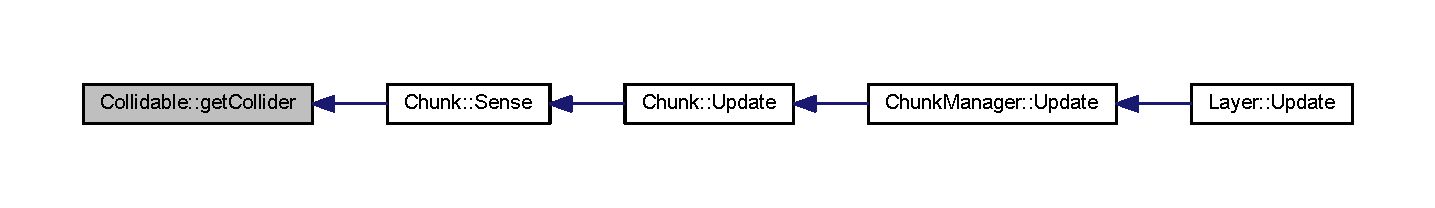
\includegraphics[width=350pt]{class_collidable_ac9edfccd8c5a1ea77238c0a19aa910c3_icgraph}
\end{center}
\end{figure}


\hypertarget{class_collidable_a8cc1f09ce02e6fcf56d98f07f908a104}{\index{Collidable@{Collidable}!is\-Moved@{is\-Moved}}
\index{is\-Moved@{is\-Moved}!Collidable@{Collidable}}
\subsubsection[{is\-Moved}]{\setlength{\rightskip}{0pt plus 5cm}bool Collidable\-::is\-Moved (
\begin{DoxyParamCaption}
{}
\end{DoxyParamCaption}
)}}\label{class_collidable_a8cc1f09ce02e6fcf56d98f07f908a104}


\subsection{Member Data Documentation}
\hypertarget{class_collidable_a0a81575218d87940935d70800f7d663e}{\index{Collidable@{Collidable}!Collider@{Collider}}
\index{Collider@{Collider}!Collidable@{Collidable}}
\subsubsection[{Collider}]{\setlength{\rightskip}{0pt plus 5cm}{\bf Rectangle} Collidable\-::\-Collider\hspace{0.3cm}{\ttfamily [protected]}}}\label{class_collidable_a0a81575218d87940935d70800f7d663e}
\hypertarget{class_collidable_afe5442fd3a82abe62b95e93248d5f4a1}{\index{Collidable@{Collidable}!has\-Moved@{has\-Moved}}
\index{has\-Moved@{has\-Moved}!Collidable@{Collidable}}
\subsubsection[{has\-Moved}]{\setlength{\rightskip}{0pt plus 5cm}bool Collidable\-::has\-Moved\hspace{0.3cm}{\ttfamily [protected]}}}\label{class_collidable_afe5442fd3a82abe62b95e93248d5f4a1}
\hypertarget{class_collidable_ae50dbf8f9d1f584d3a5d5c3445fbe786}{\index{Collidable@{Collidable}!lastpos@{lastpos}}
\index{lastpos@{lastpos}!Collidable@{Collidable}}
\subsubsection[{lastpos}]{\setlength{\rightskip}{0pt plus 5cm}sf\-::\-Vector2f Collidable\-::lastpos\hspace{0.3cm}{\ttfamily [protected]}}}\label{class_collidable_ae50dbf8f9d1f584d3a5d5c3445fbe786}
\hypertarget{class_collidable_aa6c2e113d920df8c0d5da2a244f924bd}{\index{Collidable@{Collidable}!position@{position}}
\index{position@{position}!Collidable@{Collidable}}
\subsubsection[{position}]{\setlength{\rightskip}{0pt plus 5cm}sf\-::\-Vector2f$\ast$ Collidable\-::position\hspace{0.3cm}{\ttfamily [protected]}}}\label{class_collidable_aa6c2e113d920df8c0d5da2a244f924bd}


The documentation for this class was generated from the following files\-:\begin{DoxyCompactItemize}
\item 
D\-:/\-Users/tom/\-Documents/\-Visual Studio 2013/\-Projects/\-Revelatorframework/\-Revelatorframework/\hyperlink{_collidable_8hpp}{Collidable.\-hpp}\item 
D\-:/\-Users/tom/\-Documents/\-Visual Studio 2013/\-Projects/\-Revelatorframework/\-Revelatorframework/\hyperlink{_collidable_8cpp}{Collidable.\-cpp}\end{DoxyCompactItemize}

\hypertarget{class_drawable}{\section{Drawable Class Reference}
\label{class_drawable}\index{Drawable@{Drawable}}
}


{\ttfamily \#include $<$Drawable.\-hpp$>$}



Inheritance diagram for Drawable\-:
\nopagebreak
\begin{figure}[H]
\begin{center}
\leavevmode
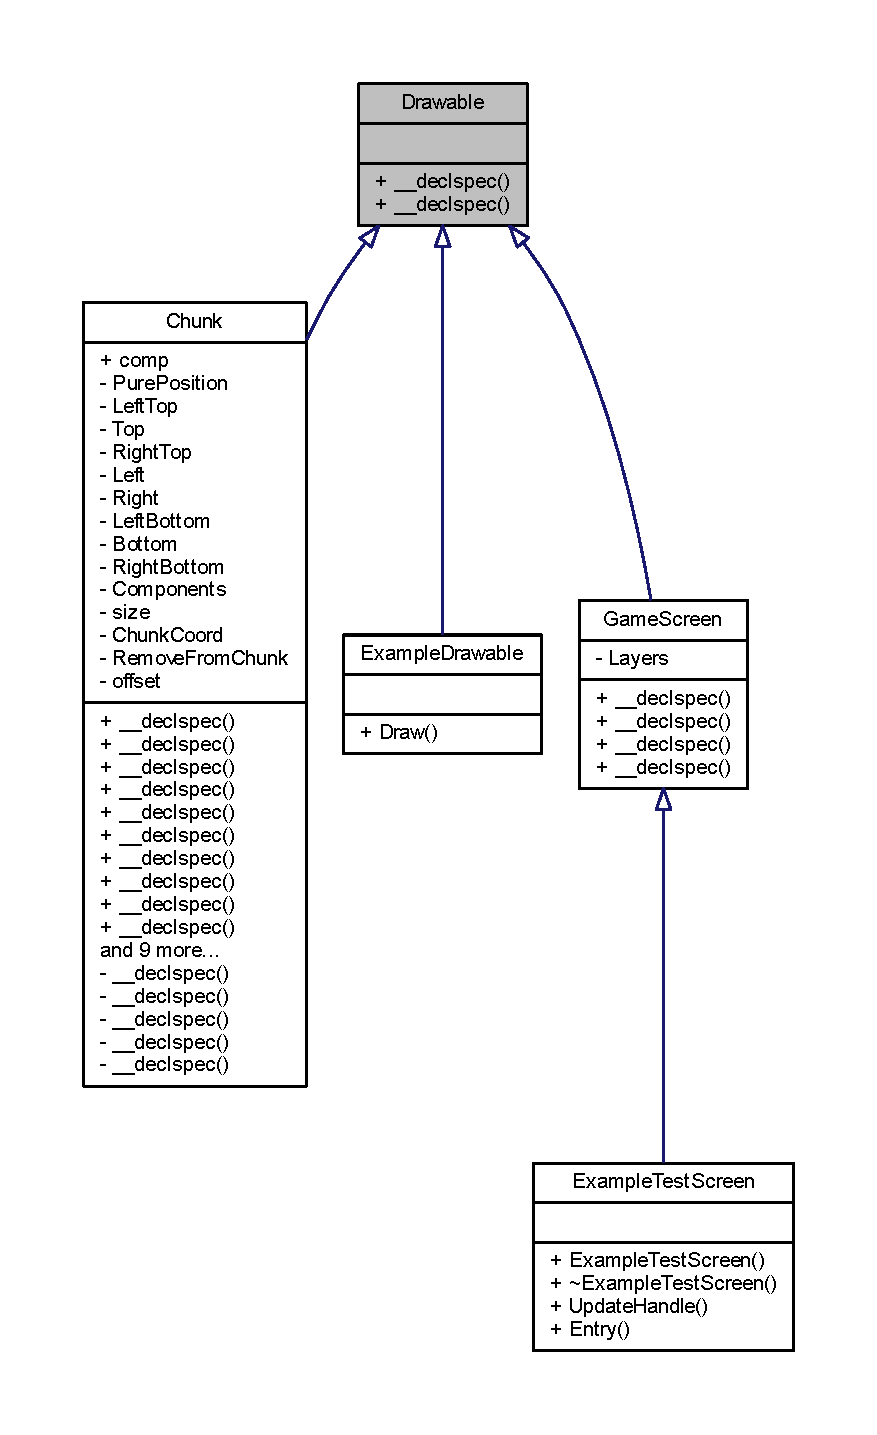
\includegraphics[height=550pt]{class_drawable__inherit__graph}
\end{center}
\end{figure}


Collaboration diagram for Drawable\-:\nopagebreak
\begin{figure}[H]
\begin{center}
\leavevmode
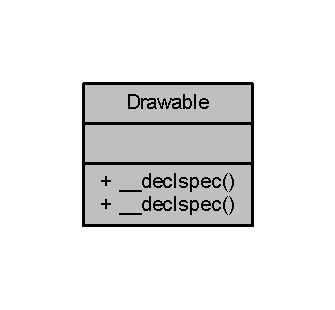
\includegraphics[width=161pt]{class_drawable__coll__graph}
\end{center}
\end{figure}
\subsection*{Public Member Functions}
\begin{DoxyCompactItemize}
\item 
\hyperlink{class_drawable_ac9f04cf11a84eb3cdf68ea48599648d7}{\-\_\-\-\_\-declspec} (dllexport) \hyperlink{class_drawable}{Drawable}()
\item 
\hyperlink{class_drawable_ab8175a6d9337a90bd36e368bd6749579}{\-\_\-\-\_\-declspec} (dllexport)$\sim$\hyperlink{class_drawable}{Drawable}()
\end{DoxyCompactItemize}


\subsection{Member Function Documentation}
\hypertarget{class_drawable_ac9f04cf11a84eb3cdf68ea48599648d7}{\index{Drawable@{Drawable}!\-\_\-\-\_\-declspec@{\-\_\-\-\_\-declspec}}
\index{\-\_\-\-\_\-declspec@{\-\_\-\-\_\-declspec}!Drawable@{Drawable}}
\subsubsection[{\-\_\-\-\_\-declspec}]{\setlength{\rightskip}{0pt plus 5cm}Drawable\-::\-\_\-\-\_\-declspec (
\begin{DoxyParamCaption}
\item[{dllexport}]{}
\end{DoxyParamCaption}
)}}\label{class_drawable_ac9f04cf11a84eb3cdf68ea48599648d7}
\hypertarget{class_drawable_ab8175a6d9337a90bd36e368bd6749579}{\index{Drawable@{Drawable}!\-\_\-\-\_\-declspec@{\-\_\-\-\_\-declspec}}
\index{\-\_\-\-\_\-declspec@{\-\_\-\-\_\-declspec}!Drawable@{Drawable}}
\subsubsection[{\-\_\-\-\_\-declspec}]{\setlength{\rightskip}{0pt plus 5cm}Drawable\-::\-\_\-\-\_\-declspec (
\begin{DoxyParamCaption}
\item[{dllexport}]{}
\end{DoxyParamCaption}
)}}\label{class_drawable_ab8175a6d9337a90bd36e368bd6749579}


The documentation for this class was generated from the following file\-:\begin{DoxyCompactItemize}
\item 
D\-:/\-Users/tom/\-Documents/\-Visual Studio 2013/\-Projects/\-Revelatorframework/\-Revelator\-Framework\-\_\-\-A\-P\-I/\hyperlink{_drawable_8hpp}{Drawable.\-hpp}\end{DoxyCompactItemize}

\hypertarget{class_example_component}{\section{Example\-Component Class Reference}
\label{class_example_component}\index{Example\-Component@{Example\-Component}}
}


{\ttfamily \#include $<$Example\-Component.\-hpp$>$}



Inheritance diagram for Example\-Component\-:\nopagebreak
\begin{figure}[H]
\begin{center}
\leavevmode
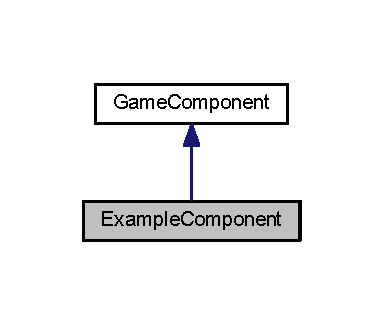
\includegraphics[width=205pt]{class_example_component__inherit__graph}
\end{center}
\end{figure}


Collaboration diagram for Example\-Component\-:
\nopagebreak
\begin{figure}[H]
\begin{center}
\leavevmode
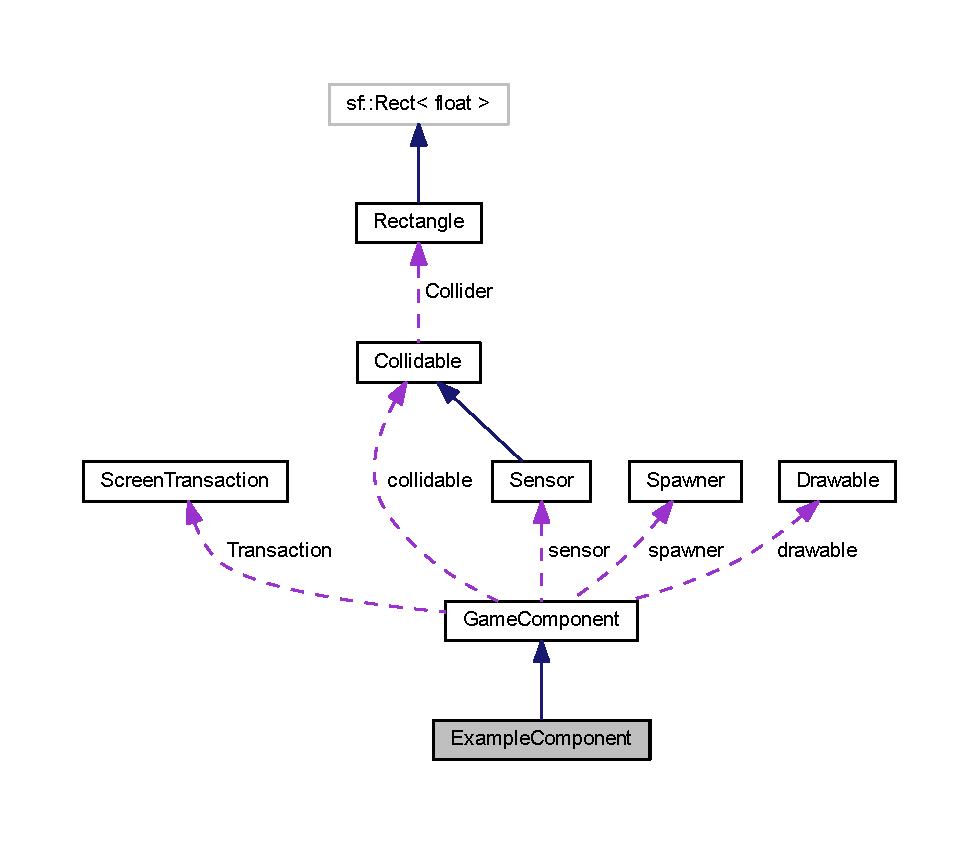
\includegraphics[width=350pt]{class_example_component__coll__graph}
\end{center}
\end{figure}
\subsection*{Public Member Functions}
\begin{DoxyCompactItemize}
\item 
\hyperlink{class_example_component_a09d97ad014e5ebe38220da6c80e96873}{Example\-Component} (sf\-::\-Vector2f pos=sf\-::\-Vector2f\{0.f, 0.f\})
\item 
void \hyperlink{class_example_component_a6ab733042d45aaa046201f486ece06b5}{Collide} (\hyperlink{class_game_component}{Game\-Component} $\ast$colider) override
\item 
\hyperlink{class_example_component_aa3a6265806020d1536d21272906181c6}{$\sim$\-Example\-Component} ()
\item 
void \hyperlink{class_example_component_a74028c9fbf9ec0fc523e60416433eacb}{Update} (\hyperlink{class_update_data}{Update\-Data} $\ast$updateobject) override
\item 
void \hyperlink{class_example_component_a385a5f04cdf04e91c8340632a1af9edc}{Draw} (sf\-::\-Render\-Window \&window, sf\-::\-Vector2f offset)
\end{DoxyCompactItemize}
\subsection*{Additional Inherited Members}


\subsection{Constructor \& Destructor Documentation}
\hypertarget{class_example_component_a09d97ad014e5ebe38220da6c80e96873}{\index{Example\-Component@{Example\-Component}!Example\-Component@{Example\-Component}}
\index{Example\-Component@{Example\-Component}!ExampleComponent@{Example\-Component}}
\subsubsection[{Example\-Component}]{\setlength{\rightskip}{0pt plus 5cm}Example\-Component\-::\-Example\-Component (
\begin{DoxyParamCaption}
\item[{sf\-::\-Vector2f}]{pos = {\ttfamily sf\-:\-:Vector2f\{0.f,0.f\}}}
\end{DoxyParamCaption}
)}}\label{class_example_component_a09d97ad014e5ebe38220da6c80e96873}
\hypertarget{class_example_component_aa3a6265806020d1536d21272906181c6}{\index{Example\-Component@{Example\-Component}!$\sim$\-Example\-Component@{$\sim$\-Example\-Component}}
\index{$\sim$\-Example\-Component@{$\sim$\-Example\-Component}!ExampleComponent@{Example\-Component}}
\subsubsection[{$\sim$\-Example\-Component}]{\setlength{\rightskip}{0pt plus 5cm}Example\-Component\-::$\sim$\-Example\-Component (
\begin{DoxyParamCaption}
{}
\end{DoxyParamCaption}
)}}\label{class_example_component_aa3a6265806020d1536d21272906181c6}


\subsection{Member Function Documentation}
\hypertarget{class_example_component_a6ab733042d45aaa046201f486ece06b5}{\index{Example\-Component@{Example\-Component}!Collide@{Collide}}
\index{Collide@{Collide}!ExampleComponent@{Example\-Component}}
\subsubsection[{Collide}]{\setlength{\rightskip}{0pt plus 5cm}void Example\-Component\-::\-Collide (
\begin{DoxyParamCaption}
\item[{{\bf Game\-Component} $\ast$}]{colider}
\end{DoxyParamCaption}
)\hspace{0.3cm}{\ttfamily [override]}}}\label{class_example_component_a6ab733042d45aaa046201f486ece06b5}
\hypertarget{class_example_component_a385a5f04cdf04e91c8340632a1af9edc}{\index{Example\-Component@{Example\-Component}!Draw@{Draw}}
\index{Draw@{Draw}!ExampleComponent@{Example\-Component}}
\subsubsection[{Draw}]{\setlength{\rightskip}{0pt plus 5cm}void Example\-Component\-::\-Draw (
\begin{DoxyParamCaption}
\item[{sf\-::\-Render\-Window \&}]{window, }
\item[{sf\-::\-Vector2f}]{offset}
\end{DoxyParamCaption}
)}}\label{class_example_component_a385a5f04cdf04e91c8340632a1af9edc}
\hypertarget{class_example_component_a74028c9fbf9ec0fc523e60416433eacb}{\index{Example\-Component@{Example\-Component}!Update@{Update}}
\index{Update@{Update}!ExampleComponent@{Example\-Component}}
\subsubsection[{Update}]{\setlength{\rightskip}{0pt plus 5cm}void Example\-Component\-::\-Update (
\begin{DoxyParamCaption}
\item[{{\bf Update\-Data} $\ast$}]{updateobject}
\end{DoxyParamCaption}
)\hspace{0.3cm}{\ttfamily [override]}}}\label{class_example_component_a74028c9fbf9ec0fc523e60416433eacb}


The documentation for this class was generated from the following files\-:\begin{DoxyCompactItemize}
\item 
D\-:/\-Users/tom/\-Documents/\-Visual Studio 2013/\-Projects/\-Revelatorframework/\-Revelatorframework/\hyperlink{_example_component_8hpp}{Example\-Component.\-hpp}\item 
D\-:/\-Users/tom/\-Documents/\-Visual Studio 2013/\-Projects/\-Revelatorframework/\-Revelatorframework/\hyperlink{_example_component_8cpp}{Example\-Component.\-cpp}\end{DoxyCompactItemize}

\hypertarget{class_example_drawable}{\section{Example\-Drawable Class Reference}
\label{class_example_drawable}\index{Example\-Drawable@{Example\-Drawable}}
}


{\ttfamily \#include $<$Example\-Component.\-hpp$>$}



Inheritance diagram for Example\-Drawable\-:\nopagebreak
\begin{figure}[H]
\begin{center}
\leavevmode
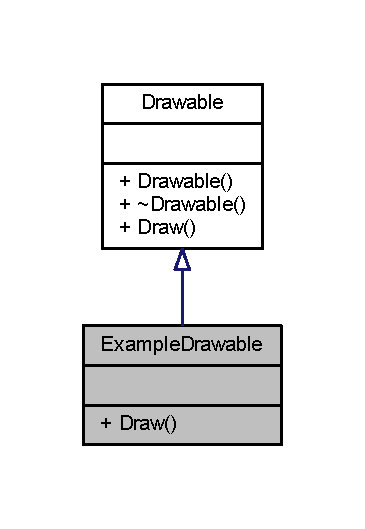
\includegraphics[width=175pt]{class_example_drawable__inherit__graph}
\end{center}
\end{figure}


Collaboration diagram for Example\-Drawable\-:\nopagebreak
\begin{figure}[H]
\begin{center}
\leavevmode
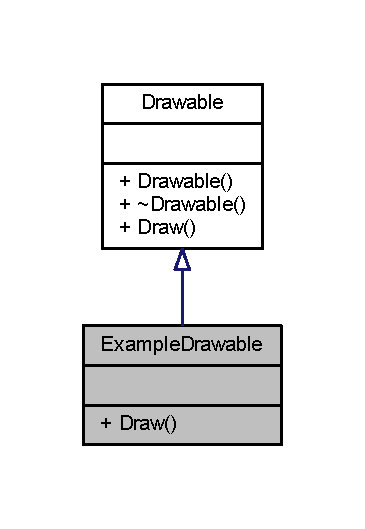
\includegraphics[width=175pt]{class_example_drawable__coll__graph}
\end{center}
\end{figure}
\subsection*{Public Member Functions}
\begin{DoxyCompactItemize}
\item 
void \hyperlink{class_example_drawable_a02efe170a267616262e1bac3d65cdf59}{Draw} (sf\-::\-Render\-Window \&window, sf\-::\-Vector2f offset) override
\end{DoxyCompactItemize}


\subsection{Member Function Documentation}
\hypertarget{class_example_drawable_a02efe170a267616262e1bac3d65cdf59}{\index{Example\-Drawable@{Example\-Drawable}!Draw@{Draw}}
\index{Draw@{Draw}!ExampleDrawable@{Example\-Drawable}}
\subsubsection[{Draw}]{\setlength{\rightskip}{0pt plus 5cm}void Example\-Drawable\-::\-Draw (
\begin{DoxyParamCaption}
\item[{sf\-::\-Render\-Window \&}]{window, }
\item[{sf\-::\-Vector2f}]{offset}
\end{DoxyParamCaption}
)\hspace{0.3cm}{\ttfamily [override]}, {\ttfamily [virtual]}}}\label{class_example_drawable_a02efe170a267616262e1bac3d65cdf59}


Implements \hyperlink{class_drawable_a0e24de52eeb44555872c70f3adf854d2}{Drawable}.



The documentation for this class was generated from the following files\-:\begin{DoxyCompactItemize}
\item 
D\-:/\-Users/tom/\-Documents/\-Visual Studio 2013/\-Projects/\-Revelatorframework/\-Revelatorframework/\hyperlink{_example_component_8hpp}{Example\-Component.\-hpp}\item 
D\-:/\-Users/tom/\-Documents/\-Visual Studio 2013/\-Projects/\-Revelatorframework/\-Revelatorframework/\hyperlink{_example_component_8cpp}{Example\-Component.\-cpp}\end{DoxyCompactItemize}

\hypertarget{class_game_component}{\section{Game\-Component Class Reference}
\label{class_game_component}\index{Game\-Component@{Game\-Component}}
}


Inheritance diagram for Game\-Component\-:\nopagebreak
\begin{figure}[H]
\begin{center}
\leavevmode
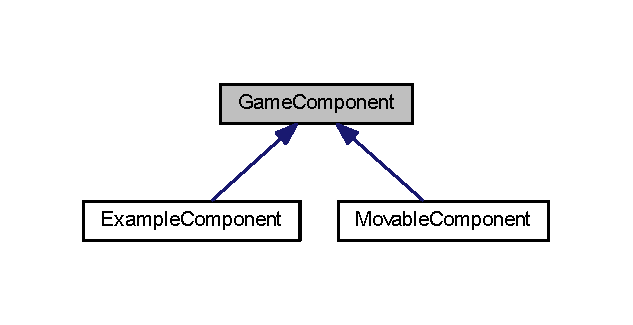
\includegraphics[width=304pt]{class_game_component__inherit__graph}
\end{center}
\end{figure}


Collaboration diagram for Game\-Component\-:\nopagebreak
\begin{figure}[H]
\begin{center}
\leavevmode
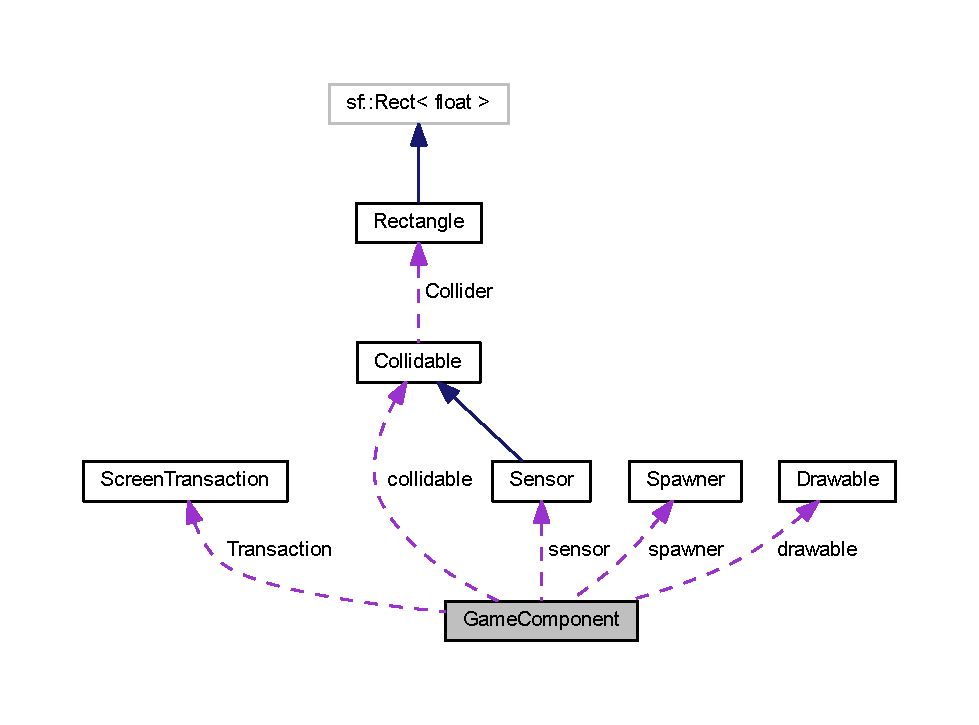
\includegraphics[width=350pt]{class_game_component__coll__graph}
\end{center}
\end{figure}
\subsection*{Public Member Functions}
\begin{DoxyCompactItemize}
\item 
\hypertarget{class_game_component_ac1eefc88d46d10f869939a7bab5a498b}{{\bfseries Game\-Component} (float x, float y)}\label{class_game_component_ac1eefc88d46d10f869939a7bab5a498b}

\item 
\hypertarget{class_game_component_a3338305ddce8cb75296ba23e1c29cf0f}{{\bfseries Game\-Component} (sf\-::\-Vector2f Pos)}\label{class_game_component_a3338305ddce8cb75296ba23e1c29cf0f}

\item 
\hypertarget{class_game_component_a01b3434d7bf6a63552e7ea4fd68744fe}{virtual void {\bfseries Update} (\hyperlink{class_update_data}{Update\-Data} $\ast$updateobject)=0}\label{class_game_component_a01b3434d7bf6a63552e7ea4fd68744fe}

\item 
\hypertarget{class_game_component_a333932780a30df552333d02669c593bc}{virtual void {\bfseries Collide} (\hyperlink{class_game_component}{Game\-Component} $\ast$colider)=0}\label{class_game_component_a333932780a30df552333d02669c593bc}

\item 
\hypertarget{class_game_component_a63c3e40531340490712b789d0d821743}{virtual void {\bfseries Draw} (sf\-::\-Render\-Window \&window, sf\-::\-Vector2f offset)=0}\label{class_game_component_a63c3e40531340490712b789d0d821743}

\item 
\hypertarget{class_game_component_a5dc0e3d5d8aa6be47d4392dc0ebe566d}{virtual bool {\bfseries has\-Transaction} ()}\label{class_game_component_a5dc0e3d5d8aa6be47d4392dc0ebe566d}

\item 
\hypertarget{class_game_component_a5473b7d5e5c1e6f6c94e1d665cb4623c}{virtual void {\bfseries set\-Transaction} (\hyperlink{class_screen_transaction}{Screen\-Transaction} $\ast$transaction)}\label{class_game_component_a5473b7d5e5c1e6f6c94e1d665cb4623c}

\item 
\hypertarget{class_game_component_a84b6f548c5045a179b9d2c33c3944f10}{virtual \hyperlink{class_screen_transaction}{Screen\-Transaction} $\ast$ {\bfseries get\-Transaction} ()}\label{class_game_component_a84b6f548c5045a179b9d2c33c3944f10}

\item 
\hypertarget{class_game_component_aabb5e9e8ed6aa3a82f5d5b5733bf201c}{sf\-::\-Vector2f $\ast$ {\bfseries get\-Position} ()}\label{class_game_component_aabb5e9e8ed6aa3a82f5d5b5733bf201c}

\item 
\hypertarget{class_game_component_ae1218b48879f706b5686bcedd4c51022}{void {\bfseries set\-Position} (sf\-::\-Vector2f $\ast$pos)}\label{class_game_component_ae1218b48879f706b5686bcedd4c51022}

\item 
\hypertarget{class_game_component_ae5a83de3b78cc5ce0f43316dd45de20d}{bool {\bfseries has\-Drawable} ()}\label{class_game_component_ae5a83de3b78cc5ce0f43316dd45de20d}

\item 
\hypertarget{class_game_component_a8595ee50d296557bcf1af3ba5283c311}{bool {\bfseries has\-Collidable} ()}\label{class_game_component_a8595ee50d296557bcf1af3ba5283c311}

\item 
\hypertarget{class_game_component_af61ba1bd218ff2aca92443c89375c222}{bool {\bfseries has\-Sensor} ()}\label{class_game_component_af61ba1bd218ff2aca92443c89375c222}

\item 
\hypertarget{class_game_component_ae6e938bb93586ad8820316368065c174}{bool {\bfseries has\-Spawner} ()}\label{class_game_component_ae6e938bb93586ad8820316368065c174}

\item 
\hypertarget{class_game_component_a6b5db3e878b861296d6cc3a0f4ee6528}{\hyperlink{class_drawable}{Drawable} $\ast$ {\bfseries get\-Drawable} ()}\label{class_game_component_a6b5db3e878b861296d6cc3a0f4ee6528}

\item 
\hypertarget{class_game_component_a09eae8038373202d058179080643f75b}{\hyperlink{class_collidable}{Collidable} $\ast$ {\bfseries get\-Collidable} ()}\label{class_game_component_a09eae8038373202d058179080643f75b}

\item 
\hypertarget{class_game_component_afca864b925be82f9c54711c75dc7be12}{\hyperlink{class_sensor}{Sensor} $\ast$ {\bfseries get\-Sensor} ()}\label{class_game_component_afca864b925be82f9c54711c75dc7be12}

\item 
\hypertarget{class_game_component_ab6db9e2e5f501ca360b08a7fc6a19644}{\hyperlink{class_spawner}{Spawner} $\ast$ {\bfseries get\-Spawner} ()}\label{class_game_component_ab6db9e2e5f501ca360b08a7fc6a19644}

\end{DoxyCompactItemize}
\subsection*{Protected Attributes}
\begin{DoxyCompactItemize}
\item 
\hypertarget{class_game_component_ab1037207fec65ac5fe65dec1e22f0566}{std\-::string {\bfseries Name}}\label{class_game_component_ab1037207fec65ac5fe65dec1e22f0566}

\item 
\hypertarget{class_game_component_ac8d794e78280785eb956eaff044f74b2}{int {\bfseries I\-D}}\label{class_game_component_ac8d794e78280785eb956eaff044f74b2}

\item 
\hypertarget{class_game_component_ae8c59f47f6723d108eb481a160607e98}{\hyperlink{class_screen_transaction}{Screen\-Transaction} $\ast$ {\bfseries Transaction}}\label{class_game_component_ae8c59f47f6723d108eb481a160607e98}

\item 
\hypertarget{class_game_component_acc3109bb4ae36112eb8796e067160c59}{sf\-::\-Vector2f $\ast$ {\bfseries Position}}\label{class_game_component_acc3109bb4ae36112eb8796e067160c59}

\item 
\hypertarget{class_game_component_acb73190345f4933825e9c8b8d5030438}{\hyperlink{class_drawable}{Drawable} $\ast$ {\bfseries drawable}}\label{class_game_component_acb73190345f4933825e9c8b8d5030438}

\item 
\hypertarget{class_game_component_aa91bd3600bd5964b55c7806dcfd1c862}{\hyperlink{class_collidable}{Collidable} $\ast$ {\bfseries collidable}}\label{class_game_component_aa91bd3600bd5964b55c7806dcfd1c862}

\item 
\hypertarget{class_game_component_ad585bf57df228afc83fbf777142e51bd}{\hyperlink{class_sensor}{Sensor} $\ast$ {\bfseries sensor}}\label{class_game_component_ad585bf57df228afc83fbf777142e51bd}

\item 
\hypertarget{class_game_component_a15caaab21ec2e8eb9d438a25afbef4da}{\hyperlink{class_spawner}{Spawner} $\ast$ {\bfseries spawner}}\label{class_game_component_a15caaab21ec2e8eb9d438a25afbef4da}

\end{DoxyCompactItemize}


The documentation for this class was generated from the following files\-:\begin{DoxyCompactItemize}
\item 
Revelatorfromework/Game\-Component.\-hpp\item 
Revelatorfromework/Game\-Component.\-cpp\end{DoxyCompactItemize}

\hypertarget{class_game_factory}{\section{Game\-Factory Class Reference}
\label{class_game_factory}\index{Game\-Factory@{Game\-Factory}}
}


{\ttfamily \#include $<$Game\-Factory.\-hpp$>$}



Collaboration diagram for Game\-Factory\-:\nopagebreak
\begin{figure}[H]
\begin{center}
\leavevmode
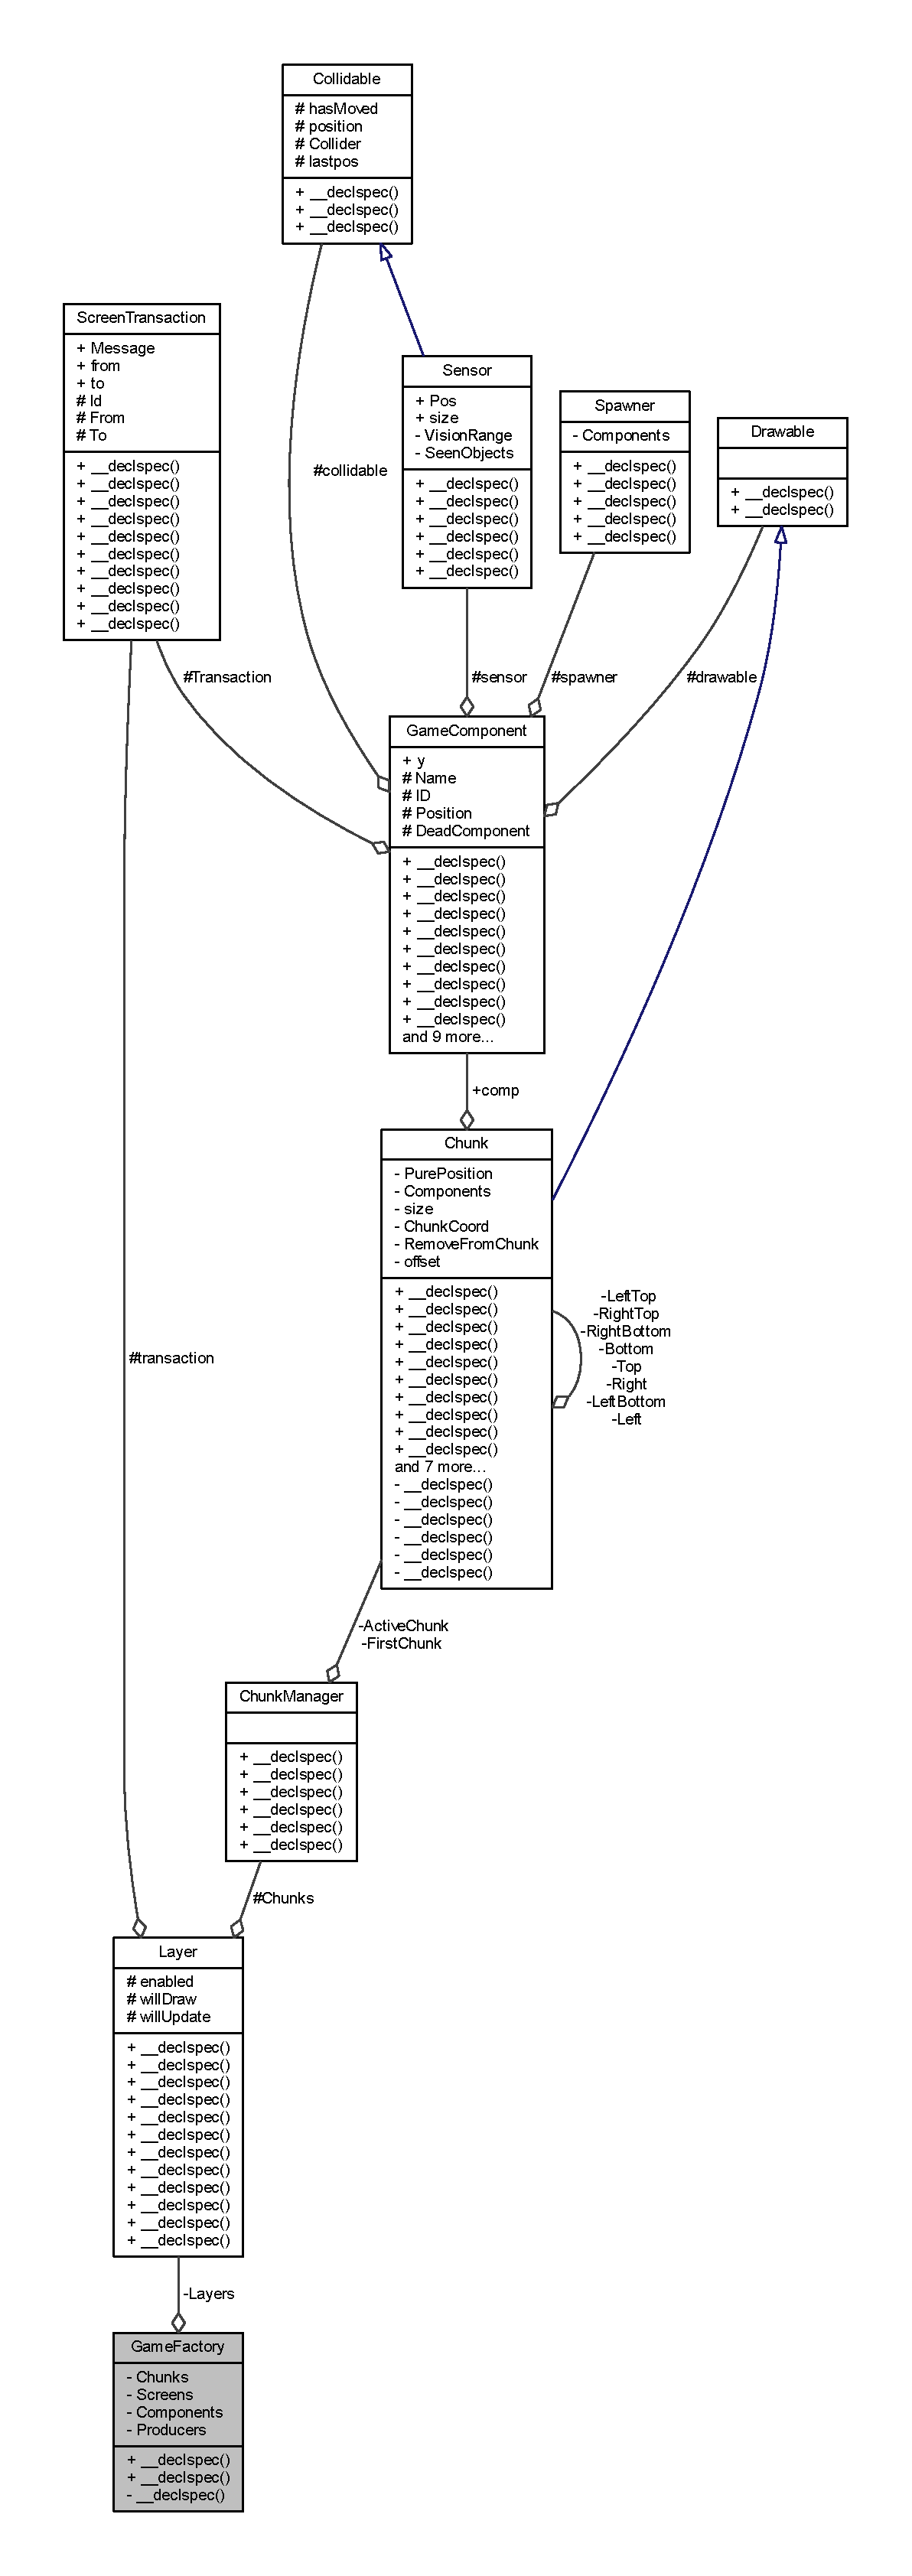
\includegraphics[width=217pt]{class_game_factory__coll__graph}
\end{center}
\end{figure}
\subsection*{Public Member Functions}
\begin{DoxyCompactItemize}
\item 
\hyperlink{class_game_factory_a0cbbb4c198cab19386d67bfe7891b785}{$\sim$\-Game\-Factory} ()
\item 
\hyperlink{class_game_screen}{Game\-Screen} $\ast$ \hyperlink{class_game_factory_ad293f5a8811d9106753916cef819fbce}{Produce\-Screen} (std\-::string screenname)
\item 
void \hyperlink{class_game_factory_a77df8b5e97869b7d7b667c0852191e20}{Register\-Object\-Producer} (std\-::string Name, \hyperlink{class_game_object_producer}{Game\-Object\-Producer} $\ast$producer)
\item 
void \hyperlink{class_game_factory_a3a20ae04c8ff992ad080b9742f5831c0}{Register\-Layer\-Producer} (std\-::string Name, \hyperlink{class_layer_producer}{Layer\-Producer} $\ast$producer)
\item 
void \hyperlink{class_game_factory_ad3c85f8654dd2c3aeb7a2b17df05cceb}{Register\-Screen\-Producer} (std\-::string Name, \hyperlink{class_game_screen_producer}{Game\-Screen\-Producer} $\ast$producer)
\item 
\hyperlink{class_game_component}{Game\-Component} $\ast$ \hyperlink{class_game_factory_a521cf5410b97240789a9cc54404d6a2f}{Produce\-Game\-Object} (std\-::string Name)
\item 
\hyperlink{class_game_component}{Game\-Component} $\ast$ \hyperlink{class_game_factory_a0ed92342411d80d6080294c29ac2c54e}{Produce\-Game\-Object} (std\-::string Name, \hyperlink{class_producer_package}{Producer\-Package} package)
\item 
void \hyperlink{class_game_factory_a7a130a6b0bff752fdd8223616a5f046f}{Delete\-Decommisioned} ()
\item 
\hyperlink{class_game_factory_a694a26c694da014dc5ced9d85a2aaaa1}{Game\-Factory} (const \hyperlink{class_game_factory}{Game\-Factory} \&utils)=delete
\item 
\hyperlink{class_game_factory}{Game\-Factory} \& \hyperlink{class_game_factory_ac9e48fb53d87829930bbc447133d9c25}{operator=} (const \hyperlink{class_game_factory}{Game\-Factory} \&utils)=delete
\end{DoxyCompactItemize}
\subsection*{Static Public Member Functions}
\begin{DoxyCompactItemize}
\item 
static \hyperlink{class_game_factory}{Game\-Factory} \& \hyperlink{class_game_factory_a0b1eef0e66b8f6ff8277f6d5fb4b8e0d}{get\-Instance} ()
\end{DoxyCompactItemize}
\subsection*{Private Member Functions}
\begin{DoxyCompactItemize}
\item 
\hyperlink{class_game_factory_a37c039131801be05d138bd76bb125ab3}{Game\-Factory} ()
\item 
\hyperlink{class_layer}{Layer} $\ast$ \hyperlink{class_game_factory_a0c24ad925bf672c6fb721dfaaf993f9d}{Produce\-Layer} (std\-::string layername, int Chunk\-Size, const int \hyperlink{class_game_factory_a77496a7ea1e2fa54acb18c499b3bd3bb}{Chunks}, bool enabled, bool willupdate, bool willdraw, \hyperlink{class_producer_package}{Producer\-Package} package, std\-::string layertype)
\end{DoxyCompactItemize}
\subsection*{Private Attributes}
\begin{DoxyCompactItemize}
\item 
std\-::list$<$ \hyperlink{class_layer}{Layer} $\ast$ $>$ \hyperlink{class_game_factory_a7ab6a968cb7af49813407fe66927c126}{Layers}
\item 
std\-::list$<$ \hyperlink{class_chunk}{Chunk} $\ast$ $>$ \hyperlink{class_game_factory_a77496a7ea1e2fa54acb18c499b3bd3bb}{Chunks}
\item 
std\-::list$<$ \hyperlink{class_game_screen}{Game\-Screen} $\ast$ $>$ \hyperlink{class_game_factory_a16a8135f6d6b1b60c0d08b39340b34cc}{Screens}
\item 
std\-::list$<$ \hyperlink{class_game_component}{Game\-Component} $\ast$ $>$ \hyperlink{class_game_factory_a90fc6360610babaf3d2d880f782772b3}{Components}
\item 
std\-::map$<$ std\-::string, \\*
\hyperlink{class_game_object_producer}{Game\-Object\-Producer} $\ast$ $>$ \hyperlink{class_game_factory_ab72819fc3f241243d44827f75e0a2886}{Object\-Producers}
\item 
std\-::map$<$ std\-::string, \\*
\hyperlink{class_game_screen_producer}{Game\-Screen\-Producer} $\ast$ $>$ \hyperlink{class_game_factory_aa65ba67e6c3fc56ec228c801e02352c8}{Screen\-Producers}
\item 
std\-::map$<$ std\-::string, \\*
\hyperlink{class_layer_producer}{Layer\-Producer} $\ast$ $>$ \hyperlink{class_game_factory_adfadca1996a3982f4b45c67ced1520f2}{Layer\-Producers}
\end{DoxyCompactItemize}


\subsection{Constructor \& Destructor Documentation}
\hypertarget{class_game_factory_a0cbbb4c198cab19386d67bfe7891b785}{\index{Game\-Factory@{Game\-Factory}!$\sim$\-Game\-Factory@{$\sim$\-Game\-Factory}}
\index{$\sim$\-Game\-Factory@{$\sim$\-Game\-Factory}!GameFactory@{Game\-Factory}}
\subsubsection[{$\sim$\-Game\-Factory}]{\setlength{\rightskip}{0pt plus 5cm}Game\-Factory\-::$\sim$\-Game\-Factory (
\begin{DoxyParamCaption}
{}
\end{DoxyParamCaption}
)}}\label{class_game_factory_a0cbbb4c198cab19386d67bfe7891b785}
\hypertarget{class_game_factory_a694a26c694da014dc5ced9d85a2aaaa1}{\index{Game\-Factory@{Game\-Factory}!Game\-Factory@{Game\-Factory}}
\index{Game\-Factory@{Game\-Factory}!GameFactory@{Game\-Factory}}
\subsubsection[{Game\-Factory}]{\setlength{\rightskip}{0pt plus 5cm}Game\-Factory\-::\-Game\-Factory (
\begin{DoxyParamCaption}
\item[{const {\bf Game\-Factory} \&}]{utils}
\end{DoxyParamCaption}
)\hspace{0.3cm}{\ttfamily [delete]}}}\label{class_game_factory_a694a26c694da014dc5ced9d85a2aaaa1}
\hypertarget{class_game_factory_a37c039131801be05d138bd76bb125ab3}{\index{Game\-Factory@{Game\-Factory}!Game\-Factory@{Game\-Factory}}
\index{Game\-Factory@{Game\-Factory}!GameFactory@{Game\-Factory}}
\subsubsection[{Game\-Factory}]{\setlength{\rightskip}{0pt plus 5cm}Game\-Factory\-::\-Game\-Factory (
\begin{DoxyParamCaption}
{}
\end{DoxyParamCaption}
)\hspace{0.3cm}{\ttfamily [private]}}}\label{class_game_factory_a37c039131801be05d138bd76bb125ab3}


\subsection{Member Function Documentation}
\hypertarget{class_game_factory_a7a130a6b0bff752fdd8223616a5f046f}{\index{Game\-Factory@{Game\-Factory}!Delete\-Decommisioned@{Delete\-Decommisioned}}
\index{Delete\-Decommisioned@{Delete\-Decommisioned}!GameFactory@{Game\-Factory}}
\subsubsection[{Delete\-Decommisioned}]{\setlength{\rightskip}{0pt plus 5cm}void Game\-Factory\-::\-Delete\-Decommisioned (
\begin{DoxyParamCaption}
{}
\end{DoxyParamCaption}
)}}\label{class_game_factory_a7a130a6b0bff752fdd8223616a5f046f}


Here is the caller graph for this function\-:\nopagebreak
\begin{figure}[H]
\begin{center}
\leavevmode
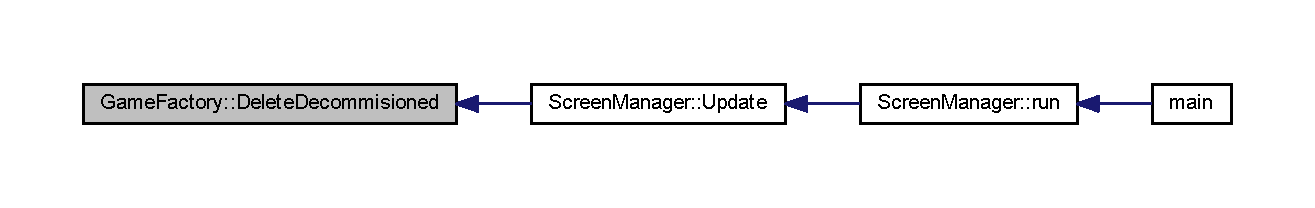
\includegraphics[width=350pt]{class_game_factory_a7a130a6b0bff752fdd8223616a5f046f_icgraph}
\end{center}
\end{figure}


\hypertarget{class_game_factory_a0b1eef0e66b8f6ff8277f6d5fb4b8e0d}{\index{Game\-Factory@{Game\-Factory}!get\-Instance@{get\-Instance}}
\index{get\-Instance@{get\-Instance}!GameFactory@{Game\-Factory}}
\subsubsection[{get\-Instance}]{\setlength{\rightskip}{0pt plus 5cm}{\bf Game\-Factory} \& Game\-Factory\-::get\-Instance (
\begin{DoxyParamCaption}
{}
\end{DoxyParamCaption}
)\hspace{0.3cm}{\ttfamily [static]}}}\label{class_game_factory_a0b1eef0e66b8f6ff8277f6d5fb4b8e0d}


Here is the caller graph for this function\-:\nopagebreak
\begin{figure}[H]
\begin{center}
\leavevmode
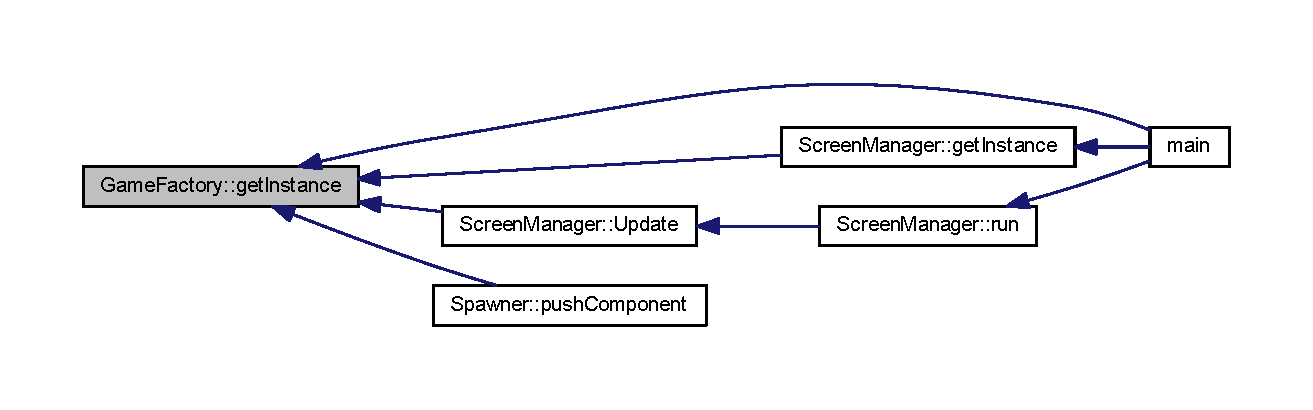
\includegraphics[width=350pt]{class_game_factory_a0b1eef0e66b8f6ff8277f6d5fb4b8e0d_icgraph}
\end{center}
\end{figure}


\hypertarget{class_game_factory_ac9e48fb53d87829930bbc447133d9c25}{\index{Game\-Factory@{Game\-Factory}!operator=@{operator=}}
\index{operator=@{operator=}!GameFactory@{Game\-Factory}}
\subsubsection[{operator=}]{\setlength{\rightskip}{0pt plus 5cm}{\bf Game\-Factory}\& Game\-Factory\-::operator= (
\begin{DoxyParamCaption}
\item[{const {\bf Game\-Factory} \&}]{utils}
\end{DoxyParamCaption}
)\hspace{0.3cm}{\ttfamily [delete]}}}\label{class_game_factory_ac9e48fb53d87829930bbc447133d9c25}
\hypertarget{class_game_factory_a521cf5410b97240789a9cc54404d6a2f}{\index{Game\-Factory@{Game\-Factory}!Produce\-Game\-Object@{Produce\-Game\-Object}}
\index{Produce\-Game\-Object@{Produce\-Game\-Object}!GameFactory@{Game\-Factory}}
\subsubsection[{Produce\-Game\-Object}]{\setlength{\rightskip}{0pt plus 5cm}{\bf Game\-Component} $\ast$ Game\-Factory\-::\-Produce\-Game\-Object (
\begin{DoxyParamCaption}
\item[{std\-::string}]{Name}
\end{DoxyParamCaption}
)}}\label{class_game_factory_a521cf5410b97240789a9cc54404d6a2f}


Here is the caller graph for this function\-:\nopagebreak
\begin{figure}[H]
\begin{center}
\leavevmode
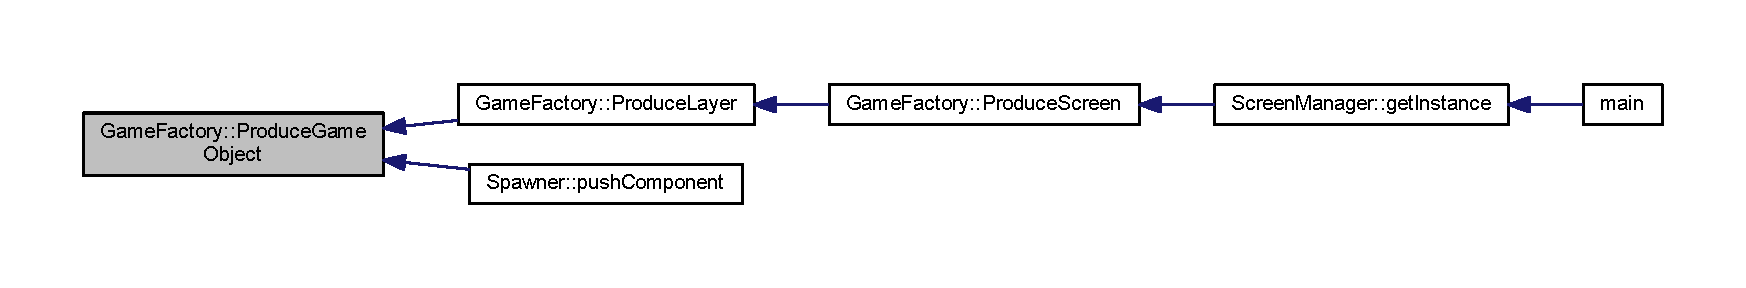
\includegraphics[width=350pt]{class_game_factory_a521cf5410b97240789a9cc54404d6a2f_icgraph}
\end{center}
\end{figure}


\hypertarget{class_game_factory_a0ed92342411d80d6080294c29ac2c54e}{\index{Game\-Factory@{Game\-Factory}!Produce\-Game\-Object@{Produce\-Game\-Object}}
\index{Produce\-Game\-Object@{Produce\-Game\-Object}!GameFactory@{Game\-Factory}}
\subsubsection[{Produce\-Game\-Object}]{\setlength{\rightskip}{0pt plus 5cm}{\bf Game\-Component} $\ast$ Game\-Factory\-::\-Produce\-Game\-Object (
\begin{DoxyParamCaption}
\item[{std\-::string}]{Name, }
\item[{{\bf Producer\-Package}}]{package}
\end{DoxyParamCaption}
)}}\label{class_game_factory_a0ed92342411d80d6080294c29ac2c54e}
\hypertarget{class_game_factory_a0c24ad925bf672c6fb721dfaaf993f9d}{\index{Game\-Factory@{Game\-Factory}!Produce\-Layer@{Produce\-Layer}}
\index{Produce\-Layer@{Produce\-Layer}!GameFactory@{Game\-Factory}}
\subsubsection[{Produce\-Layer}]{\setlength{\rightskip}{0pt plus 5cm}{\bf Layer} $\ast$ Game\-Factory\-::\-Produce\-Layer (
\begin{DoxyParamCaption}
\item[{std\-::string}]{layername, }
\item[{int}]{Chunk\-Size, }
\item[{const int}]{Chunks, }
\item[{bool}]{enabled, }
\item[{bool}]{willupdate, }
\item[{bool}]{willdraw, }
\item[{{\bf Producer\-Package}}]{package, }
\item[{std\-::string}]{layertype}
\end{DoxyParamCaption}
)\hspace{0.3cm}{\ttfamily [private]}}}\label{class_game_factory_a0c24ad925bf672c6fb721dfaaf993f9d}


Here is the call graph for this function\-:\nopagebreak
\begin{figure}[H]
\begin{center}
\leavevmode
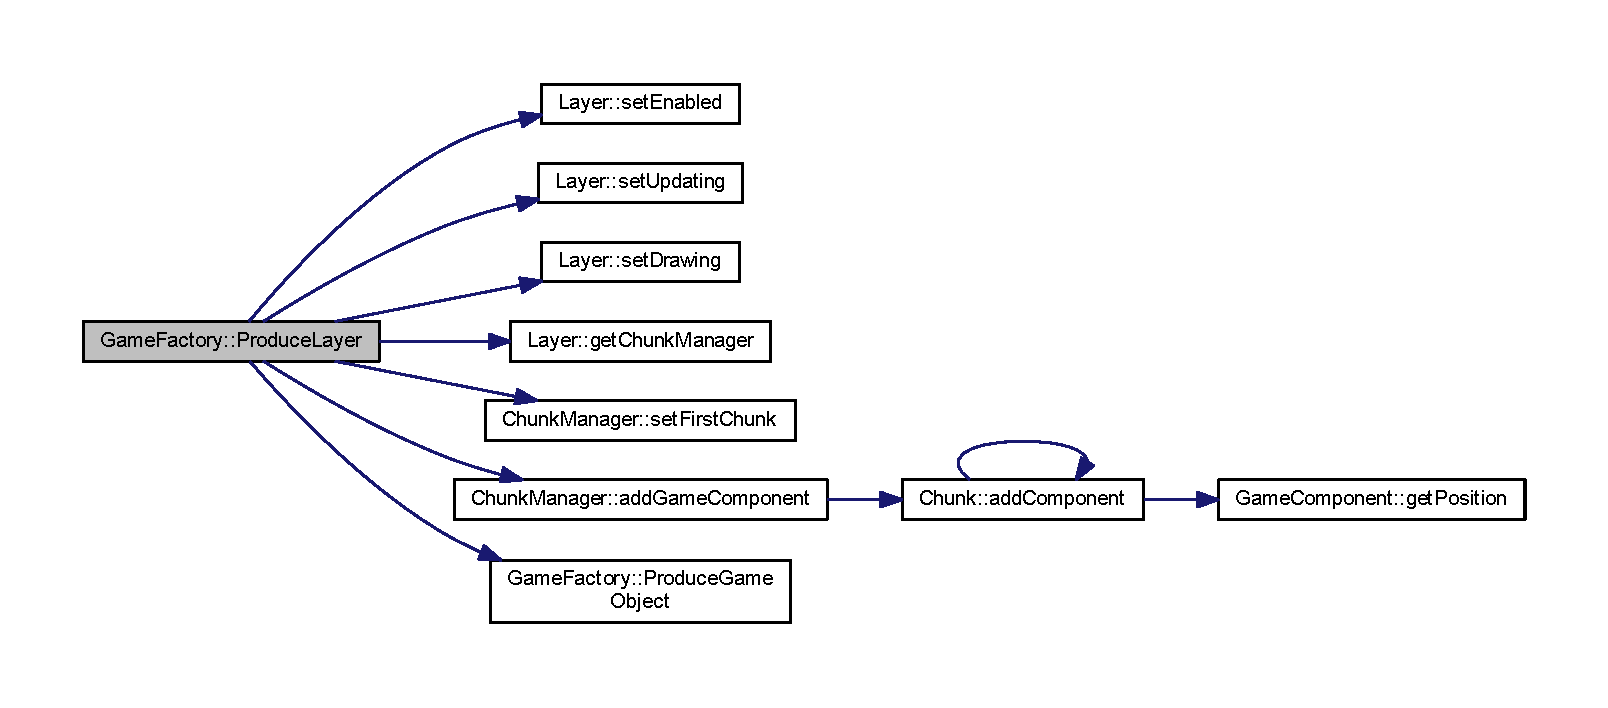
\includegraphics[width=350pt]{class_game_factory_a0c24ad925bf672c6fb721dfaaf993f9d_cgraph}
\end{center}
\end{figure}




Here is the caller graph for this function\-:\nopagebreak
\begin{figure}[H]
\begin{center}
\leavevmode
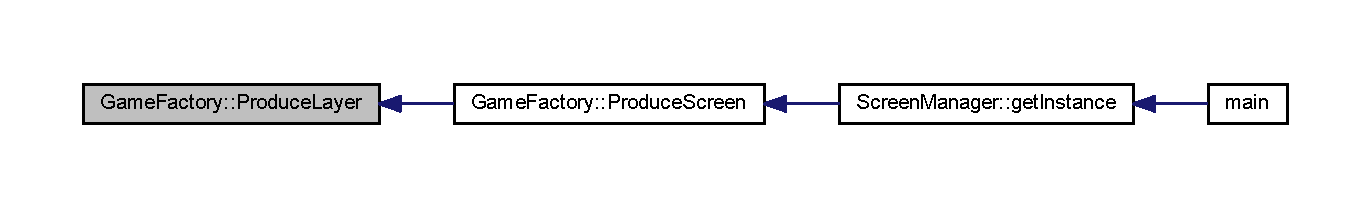
\includegraphics[width=350pt]{class_game_factory_a0c24ad925bf672c6fb721dfaaf993f9d_icgraph}
\end{center}
\end{figure}


\hypertarget{class_game_factory_ad293f5a8811d9106753916cef819fbce}{\index{Game\-Factory@{Game\-Factory}!Produce\-Screen@{Produce\-Screen}}
\index{Produce\-Screen@{Produce\-Screen}!GameFactory@{Game\-Factory}}
\subsubsection[{Produce\-Screen}]{\setlength{\rightskip}{0pt plus 5cm}{\bf Game\-Screen} $\ast$ Game\-Factory\-::\-Produce\-Screen (
\begin{DoxyParamCaption}
\item[{std\-::string}]{screenname}
\end{DoxyParamCaption}
)}}\label{class_game_factory_ad293f5a8811d9106753916cef819fbce}


Here is the call graph for this function\-:\nopagebreak
\begin{figure}[H]
\begin{center}
\leavevmode
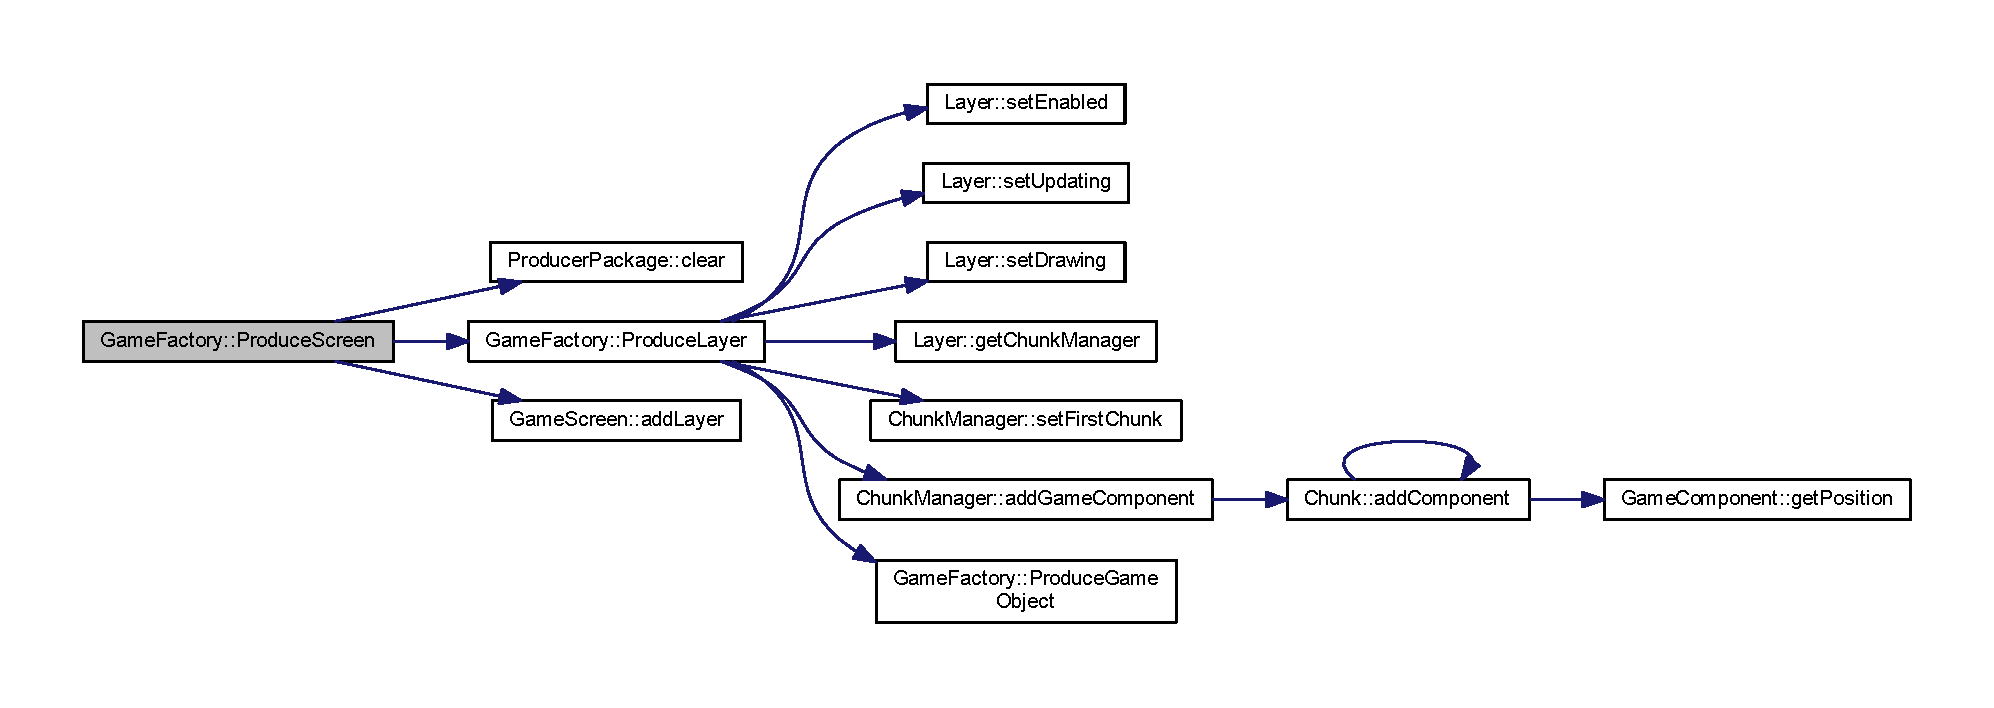
\includegraphics[width=350pt]{class_game_factory_ad293f5a8811d9106753916cef819fbce_cgraph}
\end{center}
\end{figure}




Here is the caller graph for this function\-:\nopagebreak
\begin{figure}[H]
\begin{center}
\leavevmode
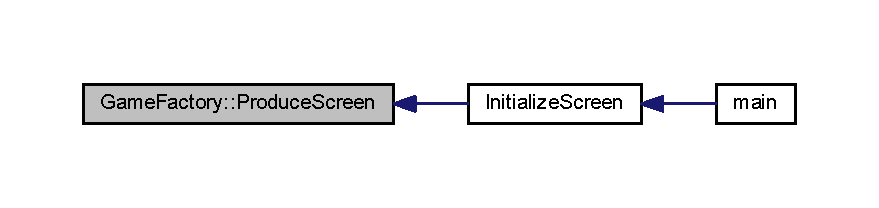
\includegraphics[width=350pt]{class_game_factory_ad293f5a8811d9106753916cef819fbce_icgraph}
\end{center}
\end{figure}


\hypertarget{class_game_factory_a3a20ae04c8ff992ad080b9742f5831c0}{\index{Game\-Factory@{Game\-Factory}!Register\-Layer\-Producer@{Register\-Layer\-Producer}}
\index{Register\-Layer\-Producer@{Register\-Layer\-Producer}!GameFactory@{Game\-Factory}}
\subsubsection[{Register\-Layer\-Producer}]{\setlength{\rightskip}{0pt plus 5cm}void Game\-Factory\-::\-Register\-Layer\-Producer (
\begin{DoxyParamCaption}
\item[{std\-::string}]{Name, }
\item[{{\bf Layer\-Producer} $\ast$}]{producer}
\end{DoxyParamCaption}
)}}\label{class_game_factory_a3a20ae04c8ff992ad080b9742f5831c0}


Here is the caller graph for this function\-:\nopagebreak
\begin{figure}[H]
\begin{center}
\leavevmode
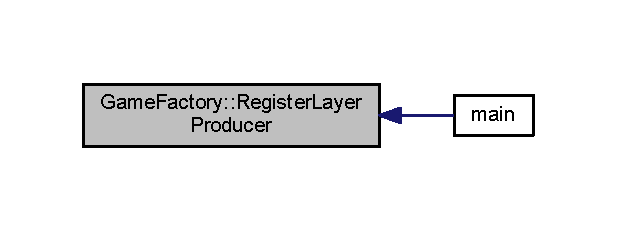
\includegraphics[width=296pt]{class_game_factory_a3a20ae04c8ff992ad080b9742f5831c0_icgraph}
\end{center}
\end{figure}


\hypertarget{class_game_factory_a77df8b5e97869b7d7b667c0852191e20}{\index{Game\-Factory@{Game\-Factory}!Register\-Object\-Producer@{Register\-Object\-Producer}}
\index{Register\-Object\-Producer@{Register\-Object\-Producer}!GameFactory@{Game\-Factory}}
\subsubsection[{Register\-Object\-Producer}]{\setlength{\rightskip}{0pt plus 5cm}void Game\-Factory\-::\-Register\-Object\-Producer (
\begin{DoxyParamCaption}
\item[{std\-::string}]{Name, }
\item[{{\bf Game\-Object\-Producer} $\ast$}]{producer}
\end{DoxyParamCaption}
)}}\label{class_game_factory_a77df8b5e97869b7d7b667c0852191e20}


Here is the caller graph for this function\-:\nopagebreak
\begin{figure}[H]
\begin{center}
\leavevmode
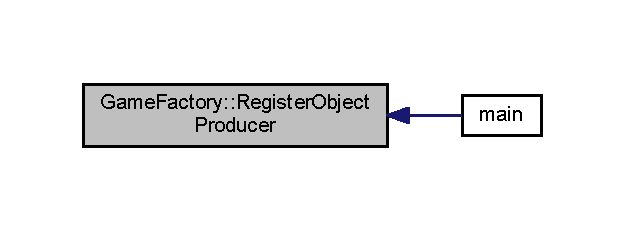
\includegraphics[width=300pt]{class_game_factory_a77df8b5e97869b7d7b667c0852191e20_icgraph}
\end{center}
\end{figure}


\hypertarget{class_game_factory_ad3c85f8654dd2c3aeb7a2b17df05cceb}{\index{Game\-Factory@{Game\-Factory}!Register\-Screen\-Producer@{Register\-Screen\-Producer}}
\index{Register\-Screen\-Producer@{Register\-Screen\-Producer}!GameFactory@{Game\-Factory}}
\subsubsection[{Register\-Screen\-Producer}]{\setlength{\rightskip}{0pt plus 5cm}void Game\-Factory\-::\-Register\-Screen\-Producer (
\begin{DoxyParamCaption}
\item[{std\-::string}]{Name, }
\item[{{\bf Game\-Screen\-Producer} $\ast$}]{producer}
\end{DoxyParamCaption}
)}}\label{class_game_factory_ad3c85f8654dd2c3aeb7a2b17df05cceb}


Here is the caller graph for this function\-:\nopagebreak
\begin{figure}[H]
\begin{center}
\leavevmode
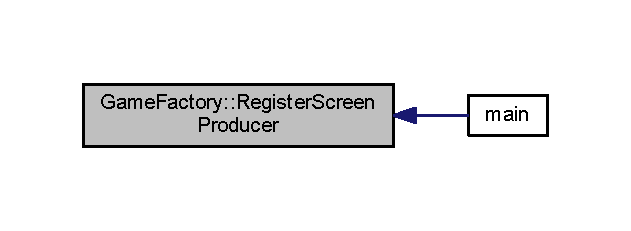
\includegraphics[width=303pt]{class_game_factory_ad3c85f8654dd2c3aeb7a2b17df05cceb_icgraph}
\end{center}
\end{figure}




\subsection{Member Data Documentation}
\hypertarget{class_game_factory_a77496a7ea1e2fa54acb18c499b3bd3bb}{\index{Game\-Factory@{Game\-Factory}!Chunks@{Chunks}}
\index{Chunks@{Chunks}!GameFactory@{Game\-Factory}}
\subsubsection[{Chunks}]{\setlength{\rightskip}{0pt plus 5cm}std\-::list$<${\bf Chunk} $\ast$$>$ Game\-Factory\-::\-Chunks\hspace{0.3cm}{\ttfamily [private]}}}\label{class_game_factory_a77496a7ea1e2fa54acb18c499b3bd3bb}
\hypertarget{class_game_factory_a90fc6360610babaf3d2d880f782772b3}{\index{Game\-Factory@{Game\-Factory}!Components@{Components}}
\index{Components@{Components}!GameFactory@{Game\-Factory}}
\subsubsection[{Components}]{\setlength{\rightskip}{0pt plus 5cm}std\-::list$<${\bf Game\-Component} $\ast$ $>$ Game\-Factory\-::\-Components\hspace{0.3cm}{\ttfamily [private]}}}\label{class_game_factory_a90fc6360610babaf3d2d880f782772b3}
\hypertarget{class_game_factory_adfadca1996a3982f4b45c67ced1520f2}{\index{Game\-Factory@{Game\-Factory}!Layer\-Producers@{Layer\-Producers}}
\index{Layer\-Producers@{Layer\-Producers}!GameFactory@{Game\-Factory}}
\subsubsection[{Layer\-Producers}]{\setlength{\rightskip}{0pt plus 5cm}std\-::map$<$std\-::string, {\bf Layer\-Producer} $\ast$$>$ Game\-Factory\-::\-Layer\-Producers\hspace{0.3cm}{\ttfamily [private]}}}\label{class_game_factory_adfadca1996a3982f4b45c67ced1520f2}
\hypertarget{class_game_factory_a7ab6a968cb7af49813407fe66927c126}{\index{Game\-Factory@{Game\-Factory}!Layers@{Layers}}
\index{Layers@{Layers}!GameFactory@{Game\-Factory}}
\subsubsection[{Layers}]{\setlength{\rightskip}{0pt plus 5cm}std\-::list$<${\bf Layer} $\ast$$>$ Game\-Factory\-::\-Layers\hspace{0.3cm}{\ttfamily [private]}}}\label{class_game_factory_a7ab6a968cb7af49813407fe66927c126}
\hypertarget{class_game_factory_ab72819fc3f241243d44827f75e0a2886}{\index{Game\-Factory@{Game\-Factory}!Object\-Producers@{Object\-Producers}}
\index{Object\-Producers@{Object\-Producers}!GameFactory@{Game\-Factory}}
\subsubsection[{Object\-Producers}]{\setlength{\rightskip}{0pt plus 5cm}std\-::map$<$std\-::string, {\bf Game\-Object\-Producer} $\ast$$>$ Game\-Factory\-::\-Object\-Producers\hspace{0.3cm}{\ttfamily [private]}}}\label{class_game_factory_ab72819fc3f241243d44827f75e0a2886}
\hypertarget{class_game_factory_aa65ba67e6c3fc56ec228c801e02352c8}{\index{Game\-Factory@{Game\-Factory}!Screen\-Producers@{Screen\-Producers}}
\index{Screen\-Producers@{Screen\-Producers}!GameFactory@{Game\-Factory}}
\subsubsection[{Screen\-Producers}]{\setlength{\rightskip}{0pt plus 5cm}std\-::map$<$std\-::string, {\bf Game\-Screen\-Producer} $\ast$$>$ Game\-Factory\-::\-Screen\-Producers\hspace{0.3cm}{\ttfamily [private]}}}\label{class_game_factory_aa65ba67e6c3fc56ec228c801e02352c8}
\hypertarget{class_game_factory_a16a8135f6d6b1b60c0d08b39340b34cc}{\index{Game\-Factory@{Game\-Factory}!Screens@{Screens}}
\index{Screens@{Screens}!GameFactory@{Game\-Factory}}
\subsubsection[{Screens}]{\setlength{\rightskip}{0pt plus 5cm}std\-::list$<${\bf Game\-Screen} $\ast$$>$ Game\-Factory\-::\-Screens\hspace{0.3cm}{\ttfamily [private]}}}\label{class_game_factory_a16a8135f6d6b1b60c0d08b39340b34cc}


The documentation for this class was generated from the following files\-:\begin{DoxyCompactItemize}
\item 
D\-:/\-Users/tom/\-Documents/\-Visual Studio 2013/\-Projects/\-Revelatorframework/\-Revelator\-Framework\-\_\-\-A\-P\-I/\hyperlink{_game_factory_8hpp}{Game\-Factory.\-hpp}\item 
D\-:/\-Users/tom/\-Documents/\-Visual Studio 2013/\-Projects/\-Revelatorframework/\-Revelator\-Framework\-\_\-\-A\-P\-I/\hyperlink{_game_factory_8cpp}{Game\-Factory.\-cpp}\end{DoxyCompactItemize}

\hypertarget{class_game_screen}{\section{Game\-Screen Class Reference}
\label{class_game_screen}\index{Game\-Screen@{Game\-Screen}}
}


{\ttfamily \#include $<$Game\-Screen.\-hpp$>$}



Inheritance diagram for Game\-Screen\-:\nopagebreak
\begin{figure}[H]
\begin{center}
\leavevmode
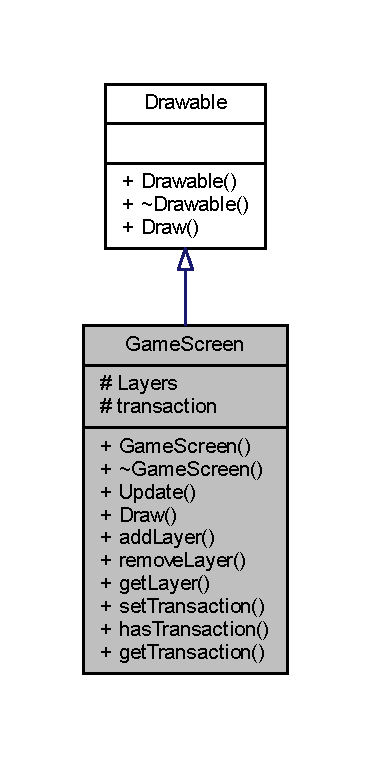
\includegraphics[width=205pt]{class_game_screen__inherit__graph}
\end{center}
\end{figure}


Collaboration diagram for Game\-Screen\-:\nopagebreak
\begin{figure}[H]
\begin{center}
\leavevmode
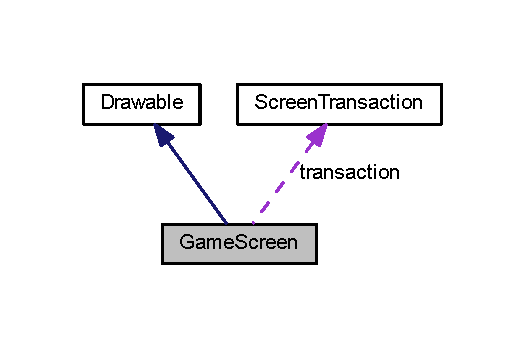
\includegraphics[width=161pt]{class_game_screen__coll__graph}
\end{center}
\end{figure}
\subsection*{Public Member Functions}
\begin{DoxyCompactItemize}
\item 
\hyperlink{class_game_screen_a41fb99405265eadec9712c99673a05f1}{\-\_\-\-\_\-declspec} (dllexport) \hyperlink{class_game_screen}{Game\-Screen}()
\item 
\hyperlink{class_game_screen_a940d1b9790ff4b737ee4c521d10a5e08}{\-\_\-\-\_\-declspec} (dllexport)$\sim$\hyperlink{class_game_screen}{Game\-Screen}()
\item 
\hyperlink{class_game_screen_a902bce77e2df723b9547d6364b5aaadf}{\-\_\-\-\_\-declspec} (dllexport) void Update(const \hyperlink{class_update_data}{Update\-Data} \&updateobject)
\item 
\hyperlink{class_game_screen_a03f75f898e71457324bd5f2cea6fc8a2}{\-\_\-\-\_\-declspec} (dllexport) virtual void Entry(\hyperlink{class_entry_object}{Entry\-Object} object)=0
\end{DoxyCompactItemize}
\subsection*{Private Attributes}
\begin{DoxyCompactItemize}
\item 
std\-::map$<$ std\-::string, \hyperlink{class_layer}{Layer} $\ast$ $>$ \hyperlink{class_game_screen_ab134d175092c247558838f11d66e9493}{Layers}
\end{DoxyCompactItemize}


\subsection{Member Function Documentation}
\hypertarget{class_game_screen_a41fb99405265eadec9712c99673a05f1}{\index{Game\-Screen@{Game\-Screen}!\-\_\-\-\_\-declspec@{\-\_\-\-\_\-declspec}}
\index{\-\_\-\-\_\-declspec@{\-\_\-\-\_\-declspec}!GameScreen@{Game\-Screen}}
\subsubsection[{\-\_\-\-\_\-declspec}]{\setlength{\rightskip}{0pt plus 5cm}Game\-Screen\-::\-\_\-\-\_\-declspec (
\begin{DoxyParamCaption}
\item[{dllexport}]{}
\end{DoxyParamCaption}
)}}\label{class_game_screen_a41fb99405265eadec9712c99673a05f1}
\hypertarget{class_game_screen_a940d1b9790ff4b737ee4c521d10a5e08}{\index{Game\-Screen@{Game\-Screen}!\-\_\-\-\_\-declspec@{\-\_\-\-\_\-declspec}}
\index{\-\_\-\-\_\-declspec@{\-\_\-\-\_\-declspec}!GameScreen@{Game\-Screen}}
\subsubsection[{\-\_\-\-\_\-declspec}]{\setlength{\rightskip}{0pt plus 5cm}Game\-Screen\-::\-\_\-\-\_\-declspec (
\begin{DoxyParamCaption}
\item[{dllexport}]{}
\end{DoxyParamCaption}
)}}\label{class_game_screen_a940d1b9790ff4b737ee4c521d10a5e08}
\hypertarget{class_game_screen_a902bce77e2df723b9547d6364b5aaadf}{\index{Game\-Screen@{Game\-Screen}!\-\_\-\-\_\-declspec@{\-\_\-\-\_\-declspec}}
\index{\-\_\-\-\_\-declspec@{\-\_\-\-\_\-declspec}!GameScreen@{Game\-Screen}}
\subsubsection[{\-\_\-\-\_\-declspec}]{\setlength{\rightskip}{0pt plus 5cm}Game\-Screen\-::\-\_\-\-\_\-declspec (
\begin{DoxyParamCaption}
\item[{dllexport}]{}
\end{DoxyParamCaption}
) const}}\label{class_game_screen_a902bce77e2df723b9547d6364b5aaadf}
\hypertarget{class_game_screen_a03f75f898e71457324bd5f2cea6fc8a2}{\index{Game\-Screen@{Game\-Screen}!\-\_\-\-\_\-declspec@{\-\_\-\-\_\-declspec}}
\index{\-\_\-\-\_\-declspec@{\-\_\-\-\_\-declspec}!GameScreen@{Game\-Screen}}
\subsubsection[{\-\_\-\-\_\-declspec}]{\setlength{\rightskip}{0pt plus 5cm}Game\-Screen\-::\-\_\-\-\_\-declspec (
\begin{DoxyParamCaption}
\item[{dllexport}]{}
\end{DoxyParamCaption}
)\hspace{0.3cm}{\ttfamily [pure virtual]}}}\label{class_game_screen_a03f75f898e71457324bd5f2cea6fc8a2}


\subsection{Member Data Documentation}
\hypertarget{class_game_screen_ab134d175092c247558838f11d66e9493}{\index{Game\-Screen@{Game\-Screen}!Layers@{Layers}}
\index{Layers@{Layers}!GameScreen@{Game\-Screen}}
\subsubsection[{Layers}]{\setlength{\rightskip}{0pt plus 5cm}std\-::map$<$std\-::string, {\bf Layer}$\ast$$>$ Game\-Screen\-::\-Layers\hspace{0.3cm}{\ttfamily [private]}}}\label{class_game_screen_ab134d175092c247558838f11d66e9493}


The documentation for this class was generated from the following file\-:\begin{DoxyCompactItemize}
\item 
D\-:/\-Users/tom/\-Documents/\-Visual Studio 2013/\-Projects/\-Revelatorframework/\-Revelator\-Framework\-\_\-\-A\-P\-I/\hyperlink{_game_screen_8hpp}{Game\-Screen.\-hpp}\end{DoxyCompactItemize}

\hypertarget{class_layer}{\section{Layer Class Reference}
\label{class_layer}\index{Layer@{Layer}}
}


{\ttfamily \#include $<$Layer.\-hpp$>$}



Inheritance diagram for Layer\-:\nopagebreak
\begin{figure}[H]
\begin{center}
\leavevmode
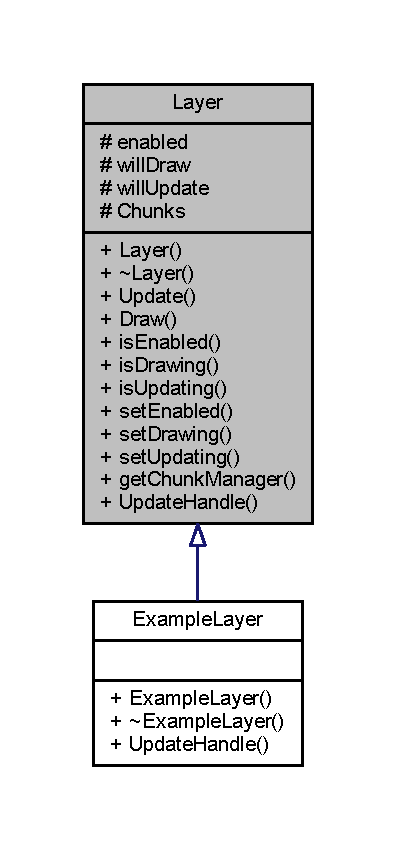
\includegraphics[width=190pt]{class_layer__inherit__graph}
\end{center}
\end{figure}


Collaboration diagram for Layer\-:\nopagebreak
\begin{figure}[H]
\begin{center}
\leavevmode
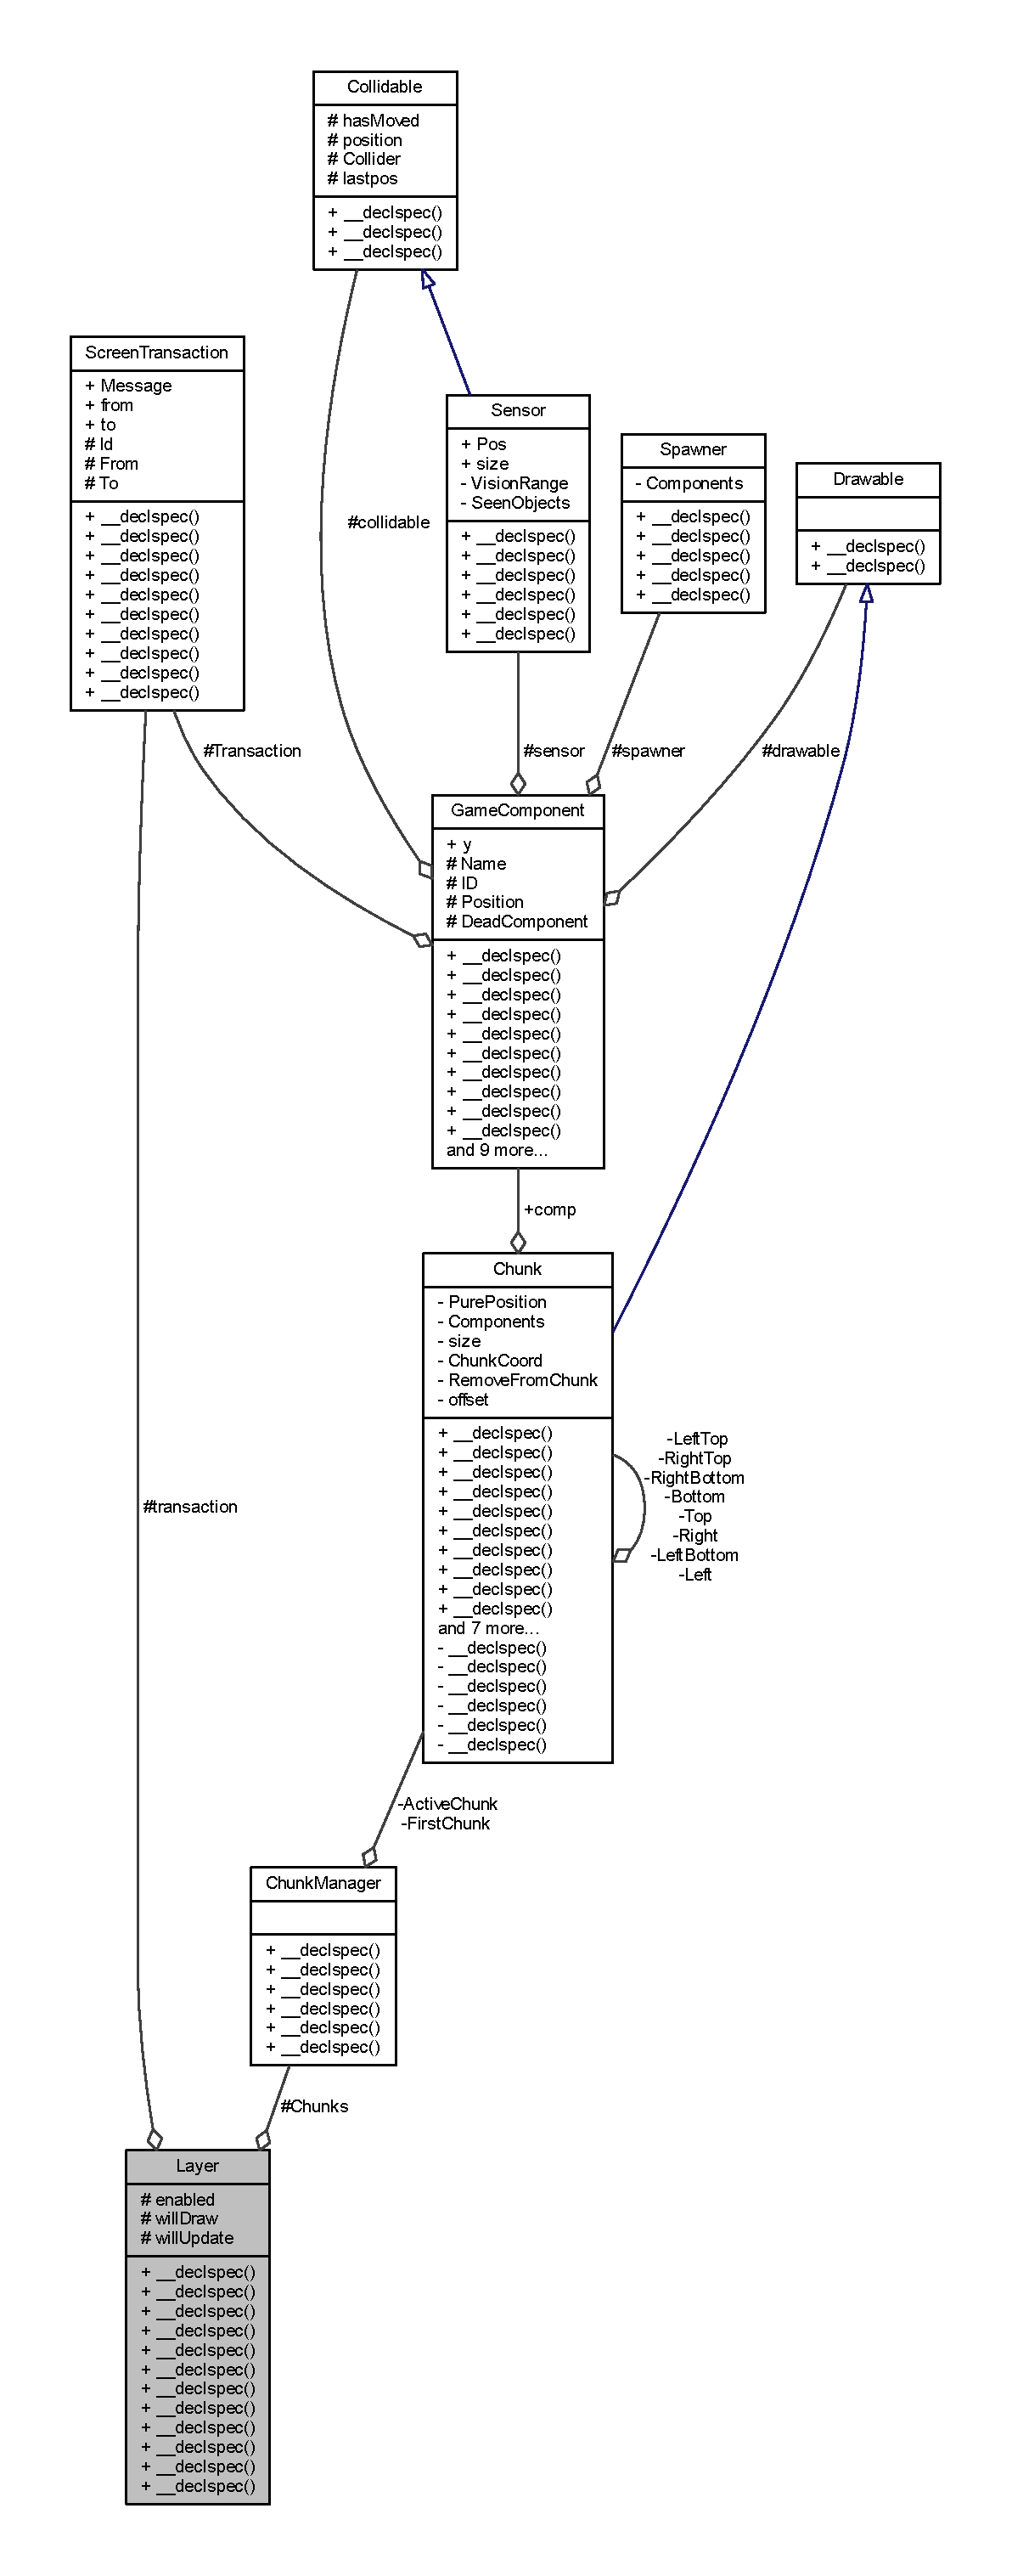
\includegraphics[height=550pt]{class_layer__coll__graph}
\end{center}
\end{figure}
\subsection*{Public Member Functions}
\begin{DoxyCompactItemize}
\item 
\hyperlink{class_layer_a8f623c7c4737dc29ecc86978d243ac6f}{Layer} ()
\item 
\hyperlink{class_layer_a1b1ba4804451dfe6cc357194e42762ae}{$\sim$\-Layer} ()
\item 
virtual void \hyperlink{class_layer_a971c3f8d301e250aded4cf0c0b9ad544}{Update} (const \hyperlink{class_update_data}{Update\-Data} \&updateobject)
\item 
virtual void \hyperlink{class_layer_a008068a5a6bd4dd274bb01bf0246cfaf}{Draw} (sf\-::\-Render\-Window \&window, sf\-::\-Vector2f offset)
\item 
bool \hyperlink{class_layer_a57c59677e3c56a7fd5e3dc985bdb9b4c}{is\-Enabled} ()
\item 
bool \hyperlink{class_layer_a46a91415e6bdc2fdb75ae0ac8498868f}{is\-Drawing} ()
\item 
bool \hyperlink{class_layer_ac2892b95b2df74446d89e4a6388f0c88}{is\-Updating} ()
\item 
void \hyperlink{class_layer_a68b9de1ac0f3eaa8274b8d0a901a825c}{set\-Enabled} (bool b)
\item 
void \hyperlink{class_layer_a0a4f62b4c031e7c2f2d5635ccd38ddd1}{set\-Drawing} (bool b)
\item 
void \hyperlink{class_layer_a0e0595efe93dbd63b05339f35399d1ad}{set\-Updating} (bool b)
\item 
\hyperlink{class_chunk_manager}{Chunk\-Manager} $\ast$ \hyperlink{class_layer_afbfd549c4d1da2e4a2d78a33586c95e1}{get\-Chunk\-Manager} ()
\item 
virtual void \hyperlink{class_layer_a1e7a6db5ee252c8ea9c44a21aaf2b0c9}{Update\-Handle} (const \hyperlink{class_update_data}{Update\-Data} \&updateobject)=0
\end{DoxyCompactItemize}
\subsection*{Protected Attributes}
\begin{DoxyCompactItemize}
\item 
bool \hyperlink{class_layer_af9f9c9a8c4a053bd829a06273df297bd}{enabled}
\item 
bool \hyperlink{class_layer_a64902a81921ba2fc792d044392b14ecc}{will\-Draw}
\item 
bool \hyperlink{class_layer_a8c3badeb437135a265c931f4ee728a48}{will\-Update}
\item 
\hyperlink{class_chunk_manager}{Chunk\-Manager} $\ast$ \hyperlink{class_layer_ab5408f6d27ad51d73df507296f16c811}{Chunks}
\end{DoxyCompactItemize}


\subsection{Constructor \& Destructor Documentation}
\hypertarget{class_layer_a8f623c7c4737dc29ecc86978d243ac6f}{\index{Layer@{Layer}!Layer@{Layer}}
\index{Layer@{Layer}!Layer@{Layer}}
\subsubsection[{Layer}]{\setlength{\rightskip}{0pt plus 5cm}Layer\-::\-Layer (
\begin{DoxyParamCaption}
{}
\end{DoxyParamCaption}
)}}\label{class_layer_a8f623c7c4737dc29ecc86978d243ac6f}
\hypertarget{class_layer_a1b1ba4804451dfe6cc357194e42762ae}{\index{Layer@{Layer}!$\sim$\-Layer@{$\sim$\-Layer}}
\index{$\sim$\-Layer@{$\sim$\-Layer}!Layer@{Layer}}
\subsubsection[{$\sim$\-Layer}]{\setlength{\rightskip}{0pt plus 5cm}Layer\-::$\sim$\-Layer (
\begin{DoxyParamCaption}
{}
\end{DoxyParamCaption}
)}}\label{class_layer_a1b1ba4804451dfe6cc357194e42762ae}


\subsection{Member Function Documentation}
\hypertarget{class_layer_a008068a5a6bd4dd274bb01bf0246cfaf}{\index{Layer@{Layer}!Draw@{Draw}}
\index{Draw@{Draw}!Layer@{Layer}}
\subsubsection[{Draw}]{\setlength{\rightskip}{0pt plus 5cm}void Layer\-::\-Draw (
\begin{DoxyParamCaption}
\item[{sf\-::\-Render\-Window \&}]{window, }
\item[{sf\-::\-Vector2f}]{offset}
\end{DoxyParamCaption}
)\hspace{0.3cm}{\ttfamily [virtual]}}}\label{class_layer_a008068a5a6bd4dd274bb01bf0246cfaf}


Here is the call graph for this function\-:\nopagebreak
\begin{figure}[H]
\begin{center}
\leavevmode
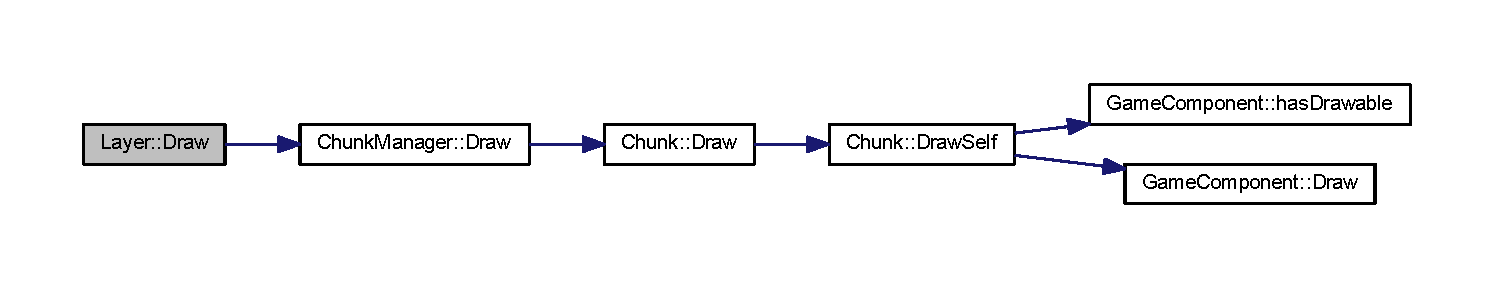
\includegraphics[width=350pt]{class_layer_a008068a5a6bd4dd274bb01bf0246cfaf_cgraph}
\end{center}
\end{figure}


\hypertarget{class_layer_afbfd549c4d1da2e4a2d78a33586c95e1}{\index{Layer@{Layer}!get\-Chunk\-Manager@{get\-Chunk\-Manager}}
\index{get\-Chunk\-Manager@{get\-Chunk\-Manager}!Layer@{Layer}}
\subsubsection[{get\-Chunk\-Manager}]{\setlength{\rightskip}{0pt plus 5cm}{\bf Chunk\-Manager}$\ast$ Layer\-::get\-Chunk\-Manager (
\begin{DoxyParamCaption}
{}
\end{DoxyParamCaption}
)\hspace{0.3cm}{\ttfamily [inline]}}}\label{class_layer_afbfd549c4d1da2e4a2d78a33586c95e1}


Here is the caller graph for this function\-:\nopagebreak
\begin{figure}[H]
\begin{center}
\leavevmode
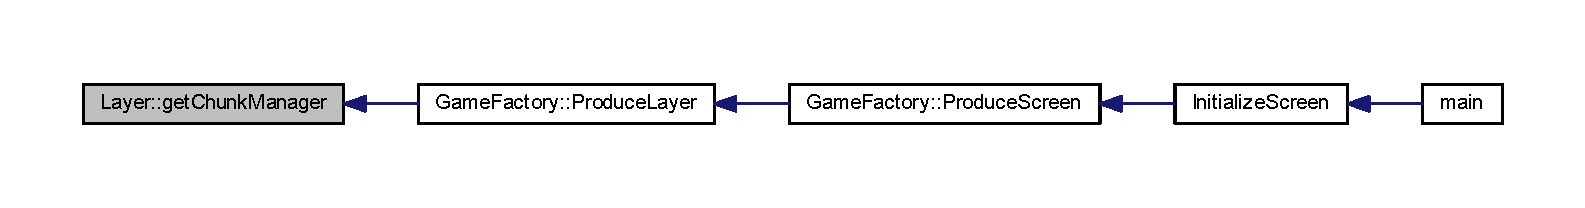
\includegraphics[width=350pt]{class_layer_afbfd549c4d1da2e4a2d78a33586c95e1_icgraph}
\end{center}
\end{figure}


\hypertarget{class_layer_a46a91415e6bdc2fdb75ae0ac8498868f}{\index{Layer@{Layer}!is\-Drawing@{is\-Drawing}}
\index{is\-Drawing@{is\-Drawing}!Layer@{Layer}}
\subsubsection[{is\-Drawing}]{\setlength{\rightskip}{0pt plus 5cm}bool Layer\-::is\-Drawing (
\begin{DoxyParamCaption}
{}
\end{DoxyParamCaption}
)\hspace{0.3cm}{\ttfamily [inline]}}}\label{class_layer_a46a91415e6bdc2fdb75ae0ac8498868f}
\hypertarget{class_layer_a57c59677e3c56a7fd5e3dc985bdb9b4c}{\index{Layer@{Layer}!is\-Enabled@{is\-Enabled}}
\index{is\-Enabled@{is\-Enabled}!Layer@{Layer}}
\subsubsection[{is\-Enabled}]{\setlength{\rightskip}{0pt plus 5cm}bool Layer\-::is\-Enabled (
\begin{DoxyParamCaption}
{}
\end{DoxyParamCaption}
)\hspace{0.3cm}{\ttfamily [inline]}}}\label{class_layer_a57c59677e3c56a7fd5e3dc985bdb9b4c}
\hypertarget{class_layer_ac2892b95b2df74446d89e4a6388f0c88}{\index{Layer@{Layer}!is\-Updating@{is\-Updating}}
\index{is\-Updating@{is\-Updating}!Layer@{Layer}}
\subsubsection[{is\-Updating}]{\setlength{\rightskip}{0pt plus 5cm}bool Layer\-::is\-Updating (
\begin{DoxyParamCaption}
{}
\end{DoxyParamCaption}
)\hspace{0.3cm}{\ttfamily [inline]}}}\label{class_layer_ac2892b95b2df74446d89e4a6388f0c88}
\hypertarget{class_layer_a0a4f62b4c031e7c2f2d5635ccd38ddd1}{\index{Layer@{Layer}!set\-Drawing@{set\-Drawing}}
\index{set\-Drawing@{set\-Drawing}!Layer@{Layer}}
\subsubsection[{set\-Drawing}]{\setlength{\rightskip}{0pt plus 5cm}void Layer\-::set\-Drawing (
\begin{DoxyParamCaption}
\item[{bool}]{b}
\end{DoxyParamCaption}
)\hspace{0.3cm}{\ttfamily [inline]}}}\label{class_layer_a0a4f62b4c031e7c2f2d5635ccd38ddd1}


Here is the caller graph for this function\-:\nopagebreak
\begin{figure}[H]
\begin{center}
\leavevmode
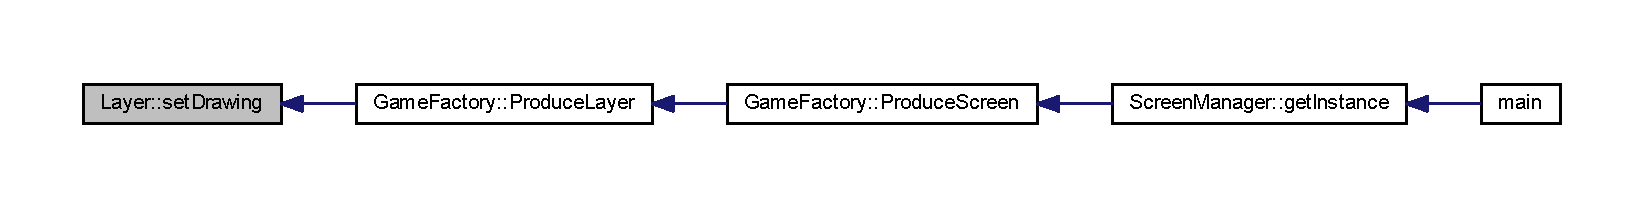
\includegraphics[width=350pt]{class_layer_a0a4f62b4c031e7c2f2d5635ccd38ddd1_icgraph}
\end{center}
\end{figure}


\hypertarget{class_layer_a68b9de1ac0f3eaa8274b8d0a901a825c}{\index{Layer@{Layer}!set\-Enabled@{set\-Enabled}}
\index{set\-Enabled@{set\-Enabled}!Layer@{Layer}}
\subsubsection[{set\-Enabled}]{\setlength{\rightskip}{0pt plus 5cm}void Layer\-::set\-Enabled (
\begin{DoxyParamCaption}
\item[{bool}]{b}
\end{DoxyParamCaption}
)\hspace{0.3cm}{\ttfamily [inline]}}}\label{class_layer_a68b9de1ac0f3eaa8274b8d0a901a825c}


Here is the caller graph for this function\-:\nopagebreak
\begin{figure}[H]
\begin{center}
\leavevmode
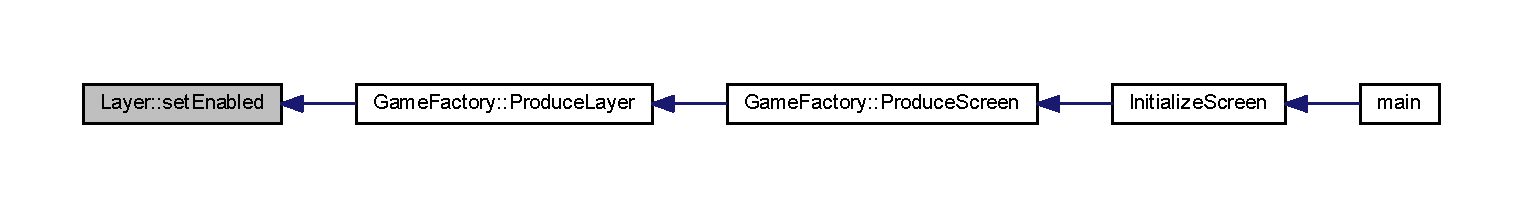
\includegraphics[width=350pt]{class_layer_a68b9de1ac0f3eaa8274b8d0a901a825c_icgraph}
\end{center}
\end{figure}


\hypertarget{class_layer_a0e0595efe93dbd63b05339f35399d1ad}{\index{Layer@{Layer}!set\-Updating@{set\-Updating}}
\index{set\-Updating@{set\-Updating}!Layer@{Layer}}
\subsubsection[{set\-Updating}]{\setlength{\rightskip}{0pt plus 5cm}void Layer\-::set\-Updating (
\begin{DoxyParamCaption}
\item[{bool}]{b}
\end{DoxyParamCaption}
)\hspace{0.3cm}{\ttfamily [inline]}}}\label{class_layer_a0e0595efe93dbd63b05339f35399d1ad}


Here is the caller graph for this function\-:\nopagebreak
\begin{figure}[H]
\begin{center}
\leavevmode
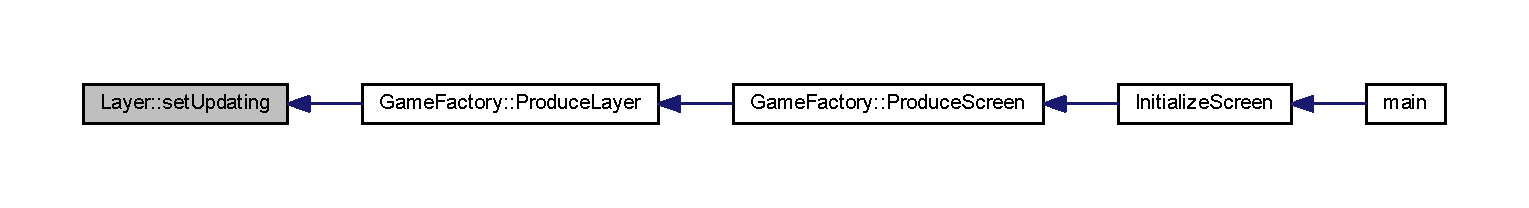
\includegraphics[width=350pt]{class_layer_a0e0595efe93dbd63b05339f35399d1ad_icgraph}
\end{center}
\end{figure}


\hypertarget{class_layer_a971c3f8d301e250aded4cf0c0b9ad544}{\index{Layer@{Layer}!Update@{Update}}
\index{Update@{Update}!Layer@{Layer}}
\subsubsection[{Update}]{\setlength{\rightskip}{0pt plus 5cm}void Layer\-::\-Update (
\begin{DoxyParamCaption}
\item[{const {\bf Update\-Data} \&}]{updateobject}
\end{DoxyParamCaption}
)\hspace{0.3cm}{\ttfamily [virtual]}}}\label{class_layer_a971c3f8d301e250aded4cf0c0b9ad544}


Here is the call graph for this function\-:\nopagebreak
\begin{figure}[H]
\begin{center}
\leavevmode
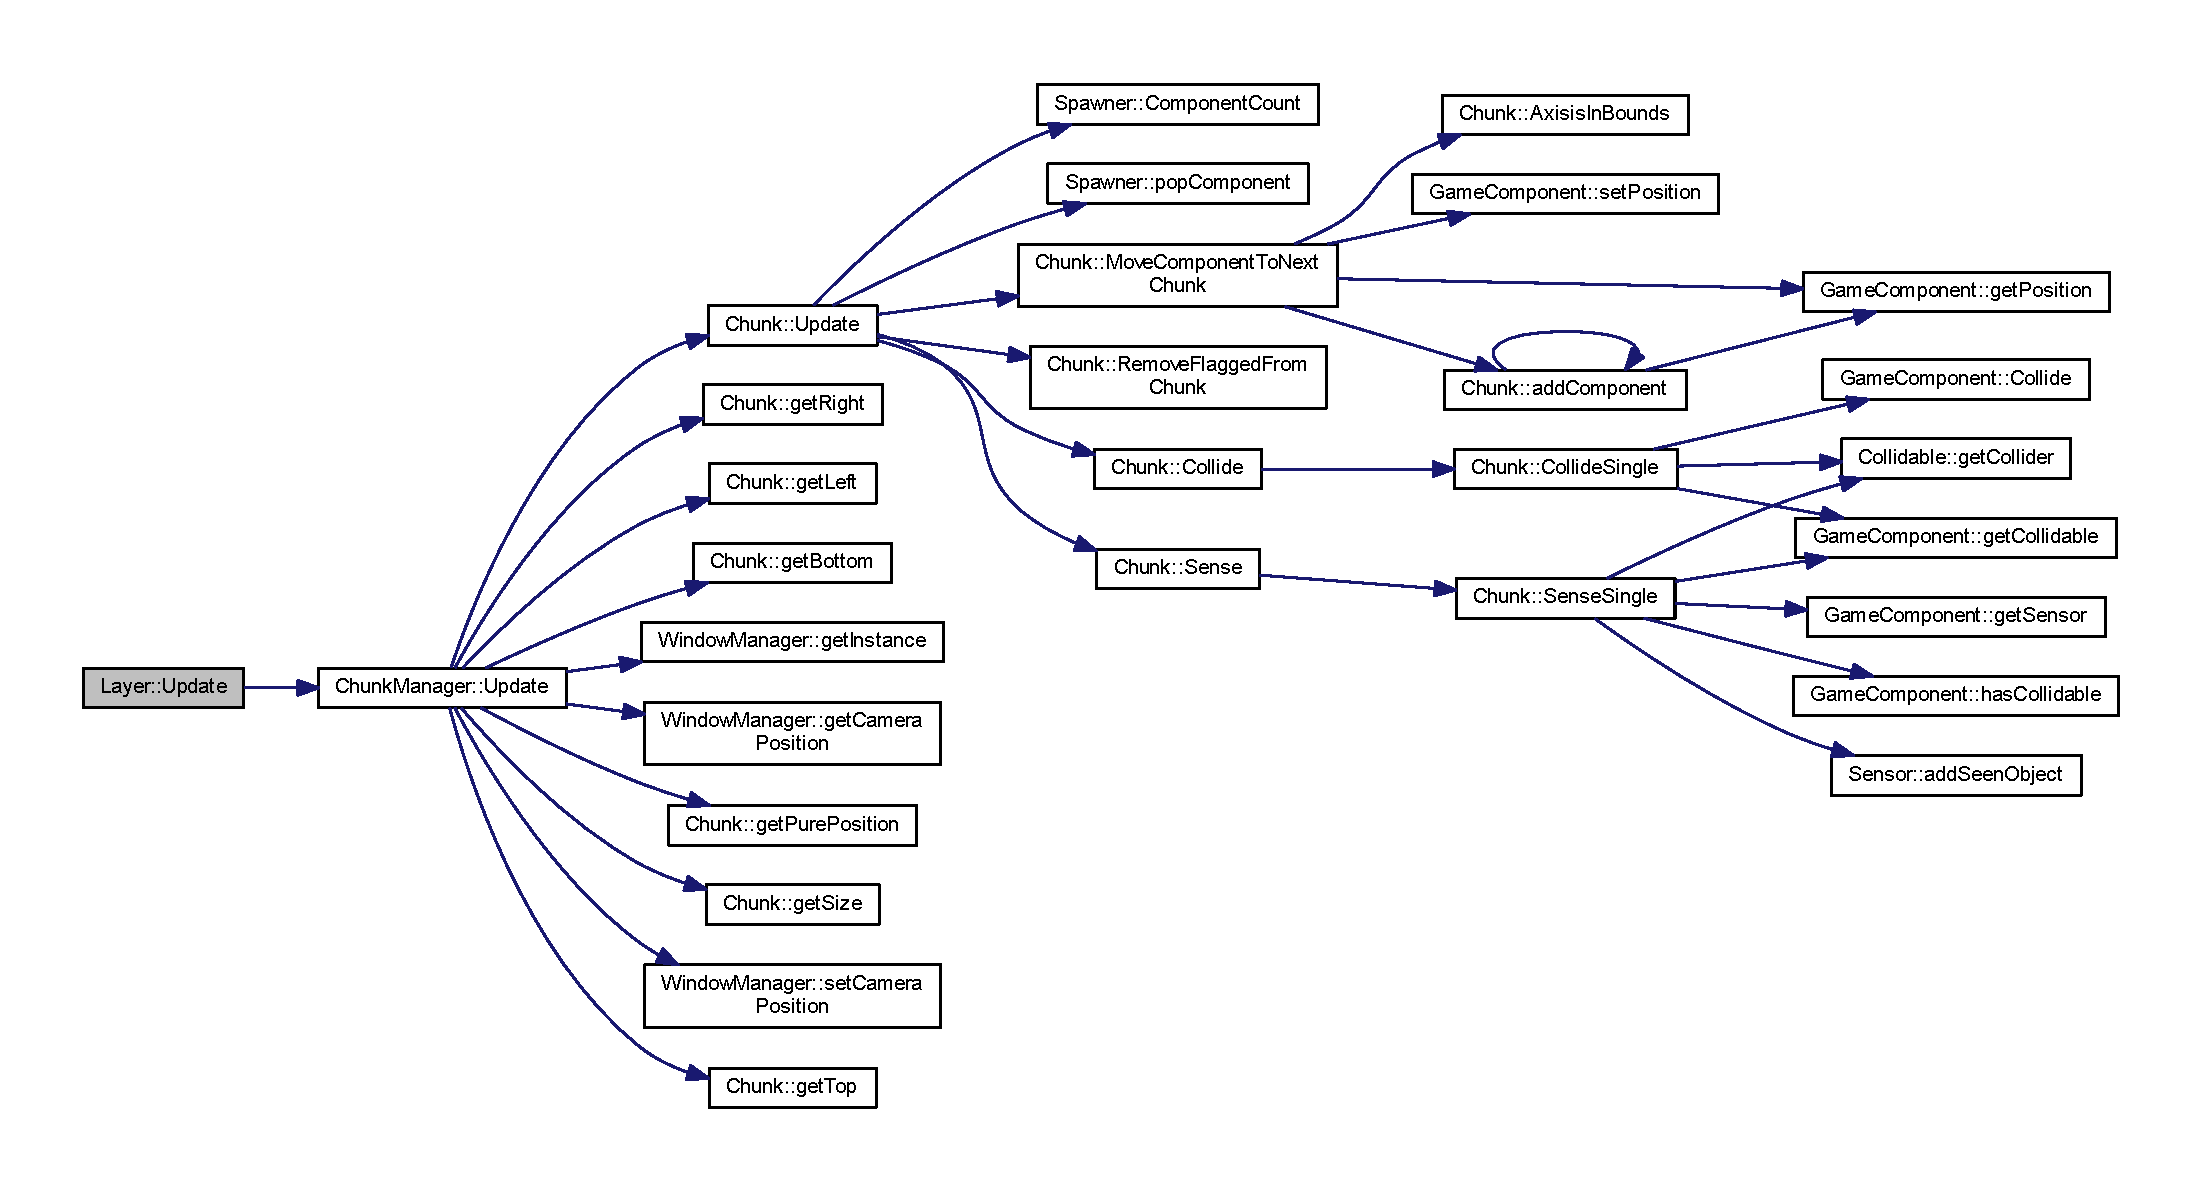
\includegraphics[width=350pt]{class_layer_a971c3f8d301e250aded4cf0c0b9ad544_cgraph}
\end{center}
\end{figure}


\hypertarget{class_layer_a1e7a6db5ee252c8ea9c44a21aaf2b0c9}{\index{Layer@{Layer}!Update\-Handle@{Update\-Handle}}
\index{Update\-Handle@{Update\-Handle}!Layer@{Layer}}
\subsubsection[{Update\-Handle}]{\setlength{\rightskip}{0pt plus 5cm}virtual void Layer\-::\-Update\-Handle (
\begin{DoxyParamCaption}
\item[{const {\bf Update\-Data} \&}]{updateobject}
\end{DoxyParamCaption}
)\hspace{0.3cm}{\ttfamily [pure virtual]}}}\label{class_layer_a1e7a6db5ee252c8ea9c44a21aaf2b0c9}


Implemented in \hyperlink{class_example_layer_a97b36d082a4b5dd7e145773fca666490}{Example\-Layer}.



\subsection{Member Data Documentation}
\hypertarget{class_layer_ab5408f6d27ad51d73df507296f16c811}{\index{Layer@{Layer}!Chunks@{Chunks}}
\index{Chunks@{Chunks}!Layer@{Layer}}
\subsubsection[{Chunks}]{\setlength{\rightskip}{0pt plus 5cm}{\bf Chunk\-Manager}$\ast$ Layer\-::\-Chunks\hspace{0.3cm}{\ttfamily [protected]}}}\label{class_layer_ab5408f6d27ad51d73df507296f16c811}
\hypertarget{class_layer_af9f9c9a8c4a053bd829a06273df297bd}{\index{Layer@{Layer}!enabled@{enabled}}
\index{enabled@{enabled}!Layer@{Layer}}
\subsubsection[{enabled}]{\setlength{\rightskip}{0pt plus 5cm}bool Layer\-::enabled\hspace{0.3cm}{\ttfamily [protected]}}}\label{class_layer_af9f9c9a8c4a053bd829a06273df297bd}
\hypertarget{class_layer_a64902a81921ba2fc792d044392b14ecc}{\index{Layer@{Layer}!will\-Draw@{will\-Draw}}
\index{will\-Draw@{will\-Draw}!Layer@{Layer}}
\subsubsection[{will\-Draw}]{\setlength{\rightskip}{0pt plus 5cm}bool Layer\-::will\-Draw\hspace{0.3cm}{\ttfamily [protected]}}}\label{class_layer_a64902a81921ba2fc792d044392b14ecc}
\hypertarget{class_layer_a8c3badeb437135a265c931f4ee728a48}{\index{Layer@{Layer}!will\-Update@{will\-Update}}
\index{will\-Update@{will\-Update}!Layer@{Layer}}
\subsubsection[{will\-Update}]{\setlength{\rightskip}{0pt plus 5cm}bool Layer\-::will\-Update\hspace{0.3cm}{\ttfamily [protected]}}}\label{class_layer_a8c3badeb437135a265c931f4ee728a48}


The documentation for this class was generated from the following files\-:\begin{DoxyCompactItemize}
\item 
D\-:/\-Users/tom/\-Documents/\-Visual Studio 2013/\-Projects/\-Revelatorframework/\-Revelator\-Framework\-\_\-\-A\-P\-I/\hyperlink{_layer_8hpp}{Layer.\-hpp}\item 
D\-:/\-Users/tom/\-Documents/\-Visual Studio 2013/\-Projects/\-Revelatorframework/\-Revelator\-Framework\-\_\-\-A\-P\-I/\hyperlink{_layer_8cpp}{Layer.\-cpp}\end{DoxyCompactItemize}

\hypertarget{class_movable_component}{\section{Movable\-Component Class Reference}
\label{class_movable_component}\index{Movable\-Component@{Movable\-Component}}
}


{\ttfamily \#include $<$Movable\-Component.\-hpp$>$}



Inheritance diagram for Movable\-Component\-:\nopagebreak
\begin{figure}[H]
\begin{center}
\leavevmode
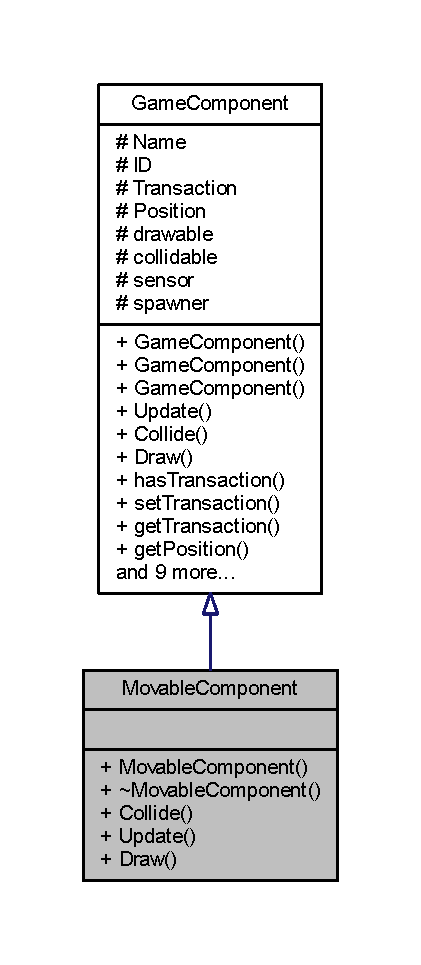
\includegraphics[width=202pt]{class_movable_component__inherit__graph}
\end{center}
\end{figure}


Collaboration diagram for Movable\-Component\-:\nopagebreak
\begin{figure}[H]
\begin{center}
\leavevmode
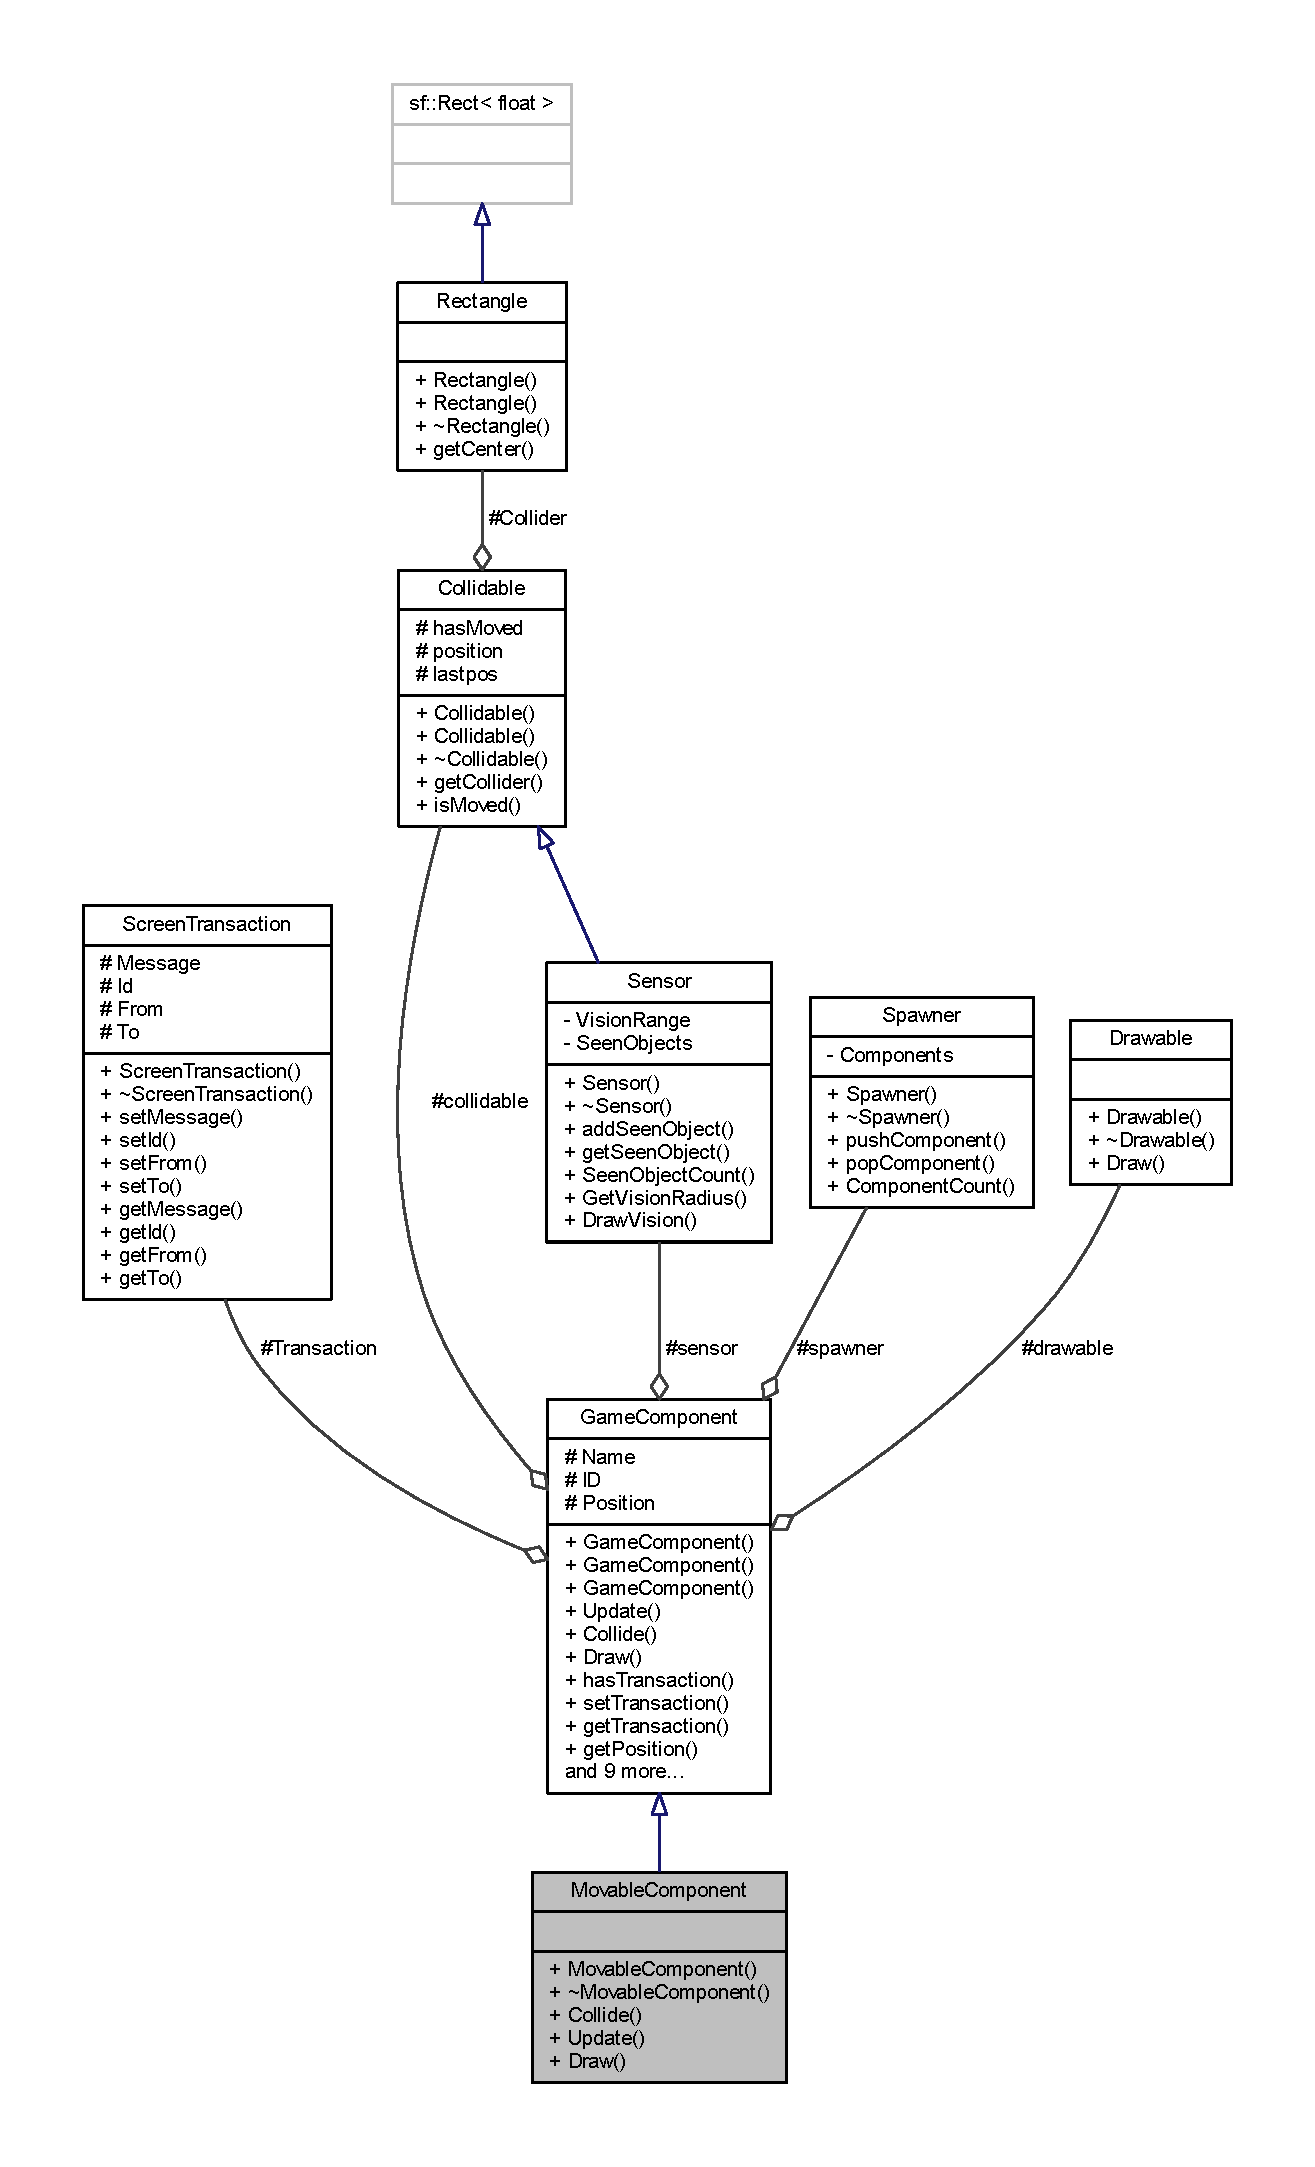
\includegraphics[height=550pt]{class_movable_component__coll__graph}
\end{center}
\end{figure}
\subsection*{Public Member Functions}
\begin{DoxyCompactItemize}
\item 
\hyperlink{class_movable_component_aea0453392e1d269a4b4c207728a3ddaf}{Movable\-Component} (sf\-::\-Vector2f pos)
\item 
\hyperlink{class_movable_component_aedc5ac024682262c99436b2b5fadddc1}{$\sim$\-Movable\-Component} ()
\item 
void \hyperlink{class_movable_component_a5ab32fd53c29a29ddcd68f1bb38a5f2b}{Collide} (\hyperlink{class_game_component}{Game\-Component} $\ast$colider) override
\item 
void \hyperlink{class_movable_component_affdc7dddf2207eda3e8a00136adf56ee}{Update} (const \hyperlink{class_update_data}{Update\-Data} \&updateobject) override
\item 
void \hyperlink{class_movable_component_a75c4dad8db642791c52d7fc5e9a92429}{Draw} (sf\-::\-Render\-Window \&window, sf\-::\-Vector2f offset)
\end{DoxyCompactItemize}
\subsection*{Additional Inherited Members}


\subsection{Constructor \& Destructor Documentation}
\hypertarget{class_movable_component_aea0453392e1d269a4b4c207728a3ddaf}{\index{Movable\-Component@{Movable\-Component}!Movable\-Component@{Movable\-Component}}
\index{Movable\-Component@{Movable\-Component}!MovableComponent@{Movable\-Component}}
\subsubsection[{Movable\-Component}]{\setlength{\rightskip}{0pt plus 5cm}Movable\-Component\-::\-Movable\-Component (
\begin{DoxyParamCaption}
\item[{sf\-::\-Vector2f}]{pos}
\end{DoxyParamCaption}
)}}\label{class_movable_component_aea0453392e1d269a4b4c207728a3ddaf}
\hypertarget{class_movable_component_aedc5ac024682262c99436b2b5fadddc1}{\index{Movable\-Component@{Movable\-Component}!$\sim$\-Movable\-Component@{$\sim$\-Movable\-Component}}
\index{$\sim$\-Movable\-Component@{$\sim$\-Movable\-Component}!MovableComponent@{Movable\-Component}}
\subsubsection[{$\sim$\-Movable\-Component}]{\setlength{\rightskip}{0pt plus 5cm}Movable\-Component\-::$\sim$\-Movable\-Component (
\begin{DoxyParamCaption}
{}
\end{DoxyParamCaption}
)}}\label{class_movable_component_aedc5ac024682262c99436b2b5fadddc1}


\subsection{Member Function Documentation}
\hypertarget{class_movable_component_a5ab32fd53c29a29ddcd68f1bb38a5f2b}{\index{Movable\-Component@{Movable\-Component}!Collide@{Collide}}
\index{Collide@{Collide}!MovableComponent@{Movable\-Component}}
\subsubsection[{Collide}]{\setlength{\rightskip}{0pt plus 5cm}void Movable\-Component\-::\-Collide (
\begin{DoxyParamCaption}
\item[{{\bf Game\-Component} $\ast$}]{colider}
\end{DoxyParamCaption}
)\hspace{0.3cm}{\ttfamily [override]}, {\ttfamily [virtual]}}}\label{class_movable_component_a5ab32fd53c29a29ddcd68f1bb38a5f2b}


Implements \hyperlink{class_game_component_a333932780a30df552333d02669c593bc}{Game\-Component}.

\hypertarget{class_movable_component_a75c4dad8db642791c52d7fc5e9a92429}{\index{Movable\-Component@{Movable\-Component}!Draw@{Draw}}
\index{Draw@{Draw}!MovableComponent@{Movable\-Component}}
\subsubsection[{Draw}]{\setlength{\rightskip}{0pt plus 5cm}void Movable\-Component\-::\-Draw (
\begin{DoxyParamCaption}
\item[{sf\-::\-Render\-Window \&}]{window, }
\item[{sf\-::\-Vector2f}]{offset}
\end{DoxyParamCaption}
)\hspace{0.3cm}{\ttfamily [virtual]}}}\label{class_movable_component_a75c4dad8db642791c52d7fc5e9a92429}


Implements \hyperlink{class_game_component_a63c3e40531340490712b789d0d821743}{Game\-Component}.



Here is the call graph for this function\-:\nopagebreak
\begin{figure}[H]
\begin{center}
\leavevmode
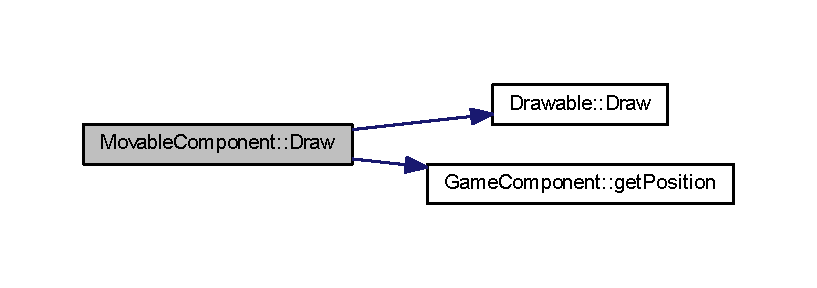
\includegraphics[width=350pt]{class_movable_component_a75c4dad8db642791c52d7fc5e9a92429_cgraph}
\end{center}
\end{figure}


\hypertarget{class_movable_component_affdc7dddf2207eda3e8a00136adf56ee}{\index{Movable\-Component@{Movable\-Component}!Update@{Update}}
\index{Update@{Update}!MovableComponent@{Movable\-Component}}
\subsubsection[{Update}]{\setlength{\rightskip}{0pt plus 5cm}void Movable\-Component\-::\-Update (
\begin{DoxyParamCaption}
\item[{const {\bf Update\-Data} \&}]{updateobject}
\end{DoxyParamCaption}
)\hspace{0.3cm}{\ttfamily [override]}, {\ttfamily [virtual]}}}\label{class_movable_component_affdc7dddf2207eda3e8a00136adf56ee}


Implements \hyperlink{class_game_component_af4ff61bad044ac587cf2f066d5b4afa0}{Game\-Component}.



Here is the call graph for this function\-:\nopagebreak
\begin{figure}[H]
\begin{center}
\leavevmode
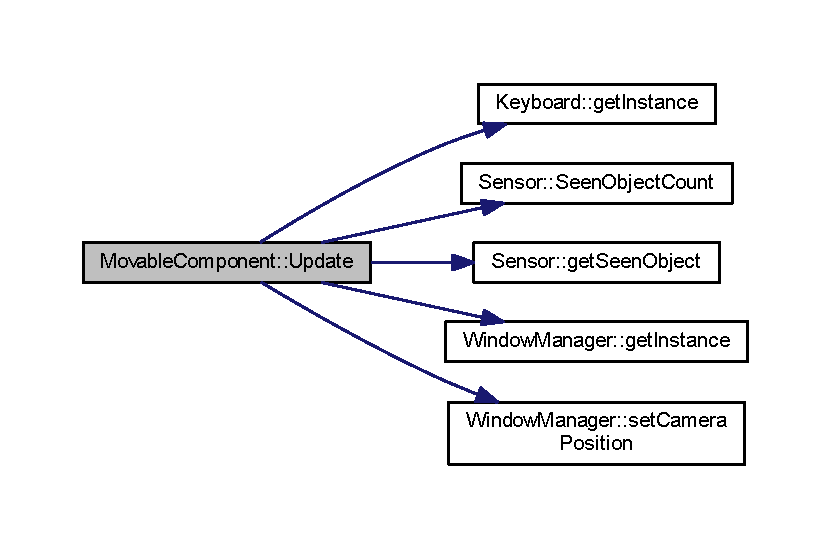
\includegraphics[width=350pt]{class_movable_component_affdc7dddf2207eda3e8a00136adf56ee_cgraph}
\end{center}
\end{figure}




The documentation for this class was generated from the following files\-:\begin{DoxyCompactItemize}
\item 
D\-:/\-Users/tom/\-Documents/\-Visual Studio 2013/\-Projects/\-Revelatorframework/\-Revelatorframework/\hyperlink{_movable_component_8hpp}{Movable\-Component.\-hpp}\item 
D\-:/\-Users/tom/\-Documents/\-Visual Studio 2013/\-Projects/\-Revelatorframework/\-Revelatorframework/\hyperlink{_movable_component_8cpp}{Movable\-Component.\-cpp}\end{DoxyCompactItemize}

\hypertarget{class_rectangle}{\section{Rectangle Class Reference}
\label{class_rectangle}\index{Rectangle@{Rectangle}}
}


{\ttfamily \#include $<$Rectangle.\-hpp$>$}



Inheritance diagram for Rectangle\-:
\nopagebreak
\begin{figure}[H]
\begin{center}
\leavevmode
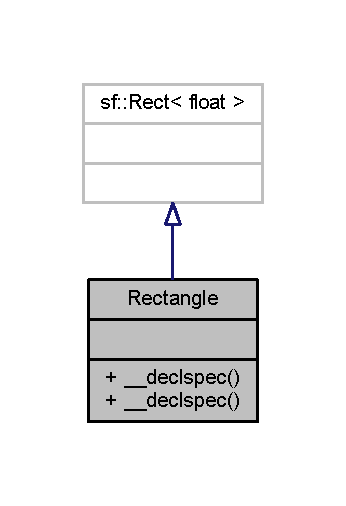
\includegraphics[width=166pt]{class_rectangle__inherit__graph}
\end{center}
\end{figure}


Collaboration diagram for Rectangle\-:
\nopagebreak
\begin{figure}[H]
\begin{center}
\leavevmode
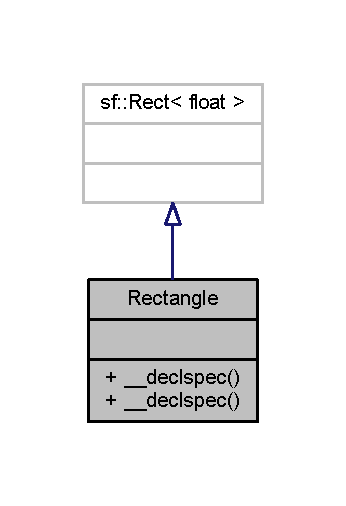
\includegraphics[width=166pt]{class_rectangle__coll__graph}
\end{center}
\end{figure}
\subsection*{Public Member Functions}
\begin{DoxyCompactItemize}
\item 
\hyperlink{class_rectangle_a67ce352978494a505456ad2119aae23e}{\-\_\-\-\_\-declspec} (dllexport) \hyperlink{class_rectangle}{Rectangle}()
\item 
\-\_\-\-\_\-declspec(dllexport) \hyperlink{class_rectangle}{Rectangle}(sf \hyperlink{class_rectangle_a6df76857725c25a783600246deaab860}{\-\_\-\-\_\-declspec} (dllexport)$\sim$\hyperlink{class_rectangle}{Rectangle}()
\end{DoxyCompactItemize}


\subsection{Member Function Documentation}
\hypertarget{class_rectangle_a67ce352978494a505456ad2119aae23e}{\index{Rectangle@{Rectangle}!\-\_\-\-\_\-declspec@{\-\_\-\-\_\-declspec}}
\index{\-\_\-\-\_\-declspec@{\-\_\-\-\_\-declspec}!Rectangle@{Rectangle}}
\subsubsection[{\-\_\-\-\_\-declspec}]{\setlength{\rightskip}{0pt plus 5cm}Rectangle\-::\-\_\-\-\_\-declspec (
\begin{DoxyParamCaption}
\item[{dllexport}]{}
\end{DoxyParamCaption}
)}}\label{class_rectangle_a67ce352978494a505456ad2119aae23e}
\hypertarget{class_rectangle_a6df76857725c25a783600246deaab860}{\index{Rectangle@{Rectangle}!\-\_\-\-\_\-declspec@{\-\_\-\-\_\-declspec}}
\index{\-\_\-\-\_\-declspec@{\-\_\-\-\_\-declspec}!Rectangle@{Rectangle}}
\subsubsection[{\-\_\-\-\_\-declspec}]{\setlength{\rightskip}{0pt plus 5cm}\-\_\-\-\_\-declspec (dllexport) {\bf Rectangle}(sf Rectangle\-::\-\_\-\-\_\-declspec (
\begin{DoxyParamCaption}
\item[{dllexport}]{}
\end{DoxyParamCaption}
)}}\label{class_rectangle_a6df76857725c25a783600246deaab860}


The documentation for this class was generated from the following file\-:\begin{DoxyCompactItemize}
\item 
D\-:/\-Users/tom/\-Documents/\-Visual Studio 2013/\-Projects/\-Revelatorframework/\-Revelator\-Framework\-\_\-\-A\-P\-I/\hyperlink{_rectangle_8hpp}{Rectangle.\-hpp}\end{DoxyCompactItemize}

\hypertarget{class_screen_manager}{\section{Screen\-Manager Class Reference}
\label{class_screen_manager}\index{Screen\-Manager@{Screen\-Manager}}
}


{\ttfamily \#include $<$Screen\-Manager.\-hpp$>$}



Collaboration diagram for Screen\-Manager\-:
\nopagebreak
\begin{figure}[H]
\begin{center}
\leavevmode
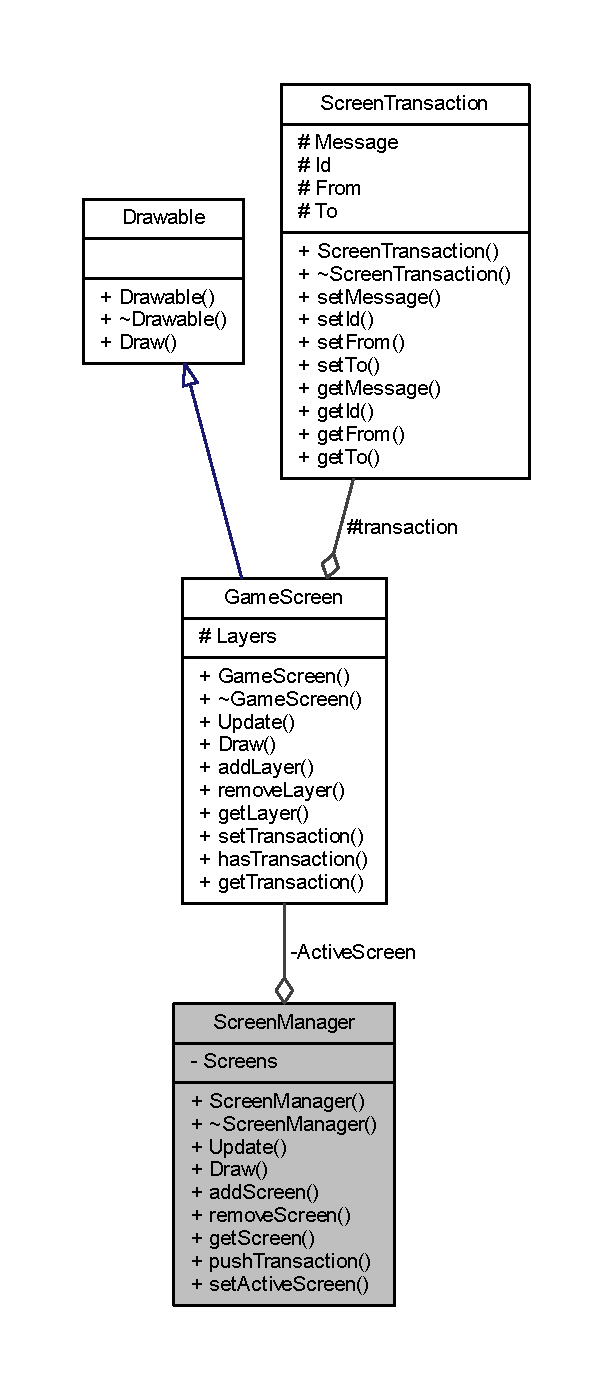
\includegraphics[height=550pt]{class_screen_manager__coll__graph}
\end{center}
\end{figure}
\subsection*{Public Member Functions}
\begin{DoxyCompactItemize}
\item 
\hyperlink{class_screen_manager_ab397f82b180ee7d50cc1e305c19ed733}{Screen\-Manager} ()
\item 
\hyperlink{class_screen_manager_a515ec6aabc9fefe3c1cfbe734877da1e}{$\sim$\-Screen\-Manager} ()
\item 
virtual void \hyperlink{class_screen_manager_a269d1b374ba195a036f03bd3caa897d9}{Update} (\hyperlink{class_update_data}{Update\-Data} $\ast$updateobject)
\item 
virtual void \hyperlink{class_screen_manager_abcf990ad052121e6ebd2ab03771657df}{Draw} (sf\-::\-Render\-Window \&window, sf\-::\-Vector2f offset)
\item 
void \hyperlink{class_screen_manager_a2e6e206c2ff265c534c802898c9c078b}{add\-Screen} (std\-::string name, \hyperlink{class_game_screen}{Game\-Screen} $\ast$screen)
\item 
void \hyperlink{class_screen_manager_a9bb115d54e94b72618361f4a347e26c8}{remove\-Screen} (std\-::string name)
\item 
\hyperlink{class_game_screen}{Game\-Screen} $\ast$ \hyperlink{class_screen_manager_a510ee04534746a6e72fa789539dc2d83}{get\-Screen} (std\-::string name)
\item 
void \hyperlink{class_screen_manager_aa806de1587575859315d975daa025688}{push\-Transaction} (\hyperlink{class_screen_transaction}{Screen\-Transaction} $\ast$transaction)
\item 
void \hyperlink{class_screen_manager_a578dea02971b86905fee58593622495b}{set\-Active\-Screen} (std\-::string name)
\end{DoxyCompactItemize}
\subsection*{Private Attributes}
\begin{DoxyCompactItemize}
\item 
std\-::map$<$ std\-::string, \\*
\hyperlink{class_game_screen}{Game\-Screen} $\ast$ $>$ \hyperlink{class_screen_manager_a54eb2c9667efda525a35d0d7043e8807}{Screens}
\item 
\hyperlink{class_game_screen}{Game\-Screen} $\ast$ \hyperlink{class_screen_manager_abb46941be1b908a2b9d8053409e89597}{Active\-Screen}
\end{DoxyCompactItemize}


\subsection{Constructor \& Destructor Documentation}
\hypertarget{class_screen_manager_ab397f82b180ee7d50cc1e305c19ed733}{\index{Screen\-Manager@{Screen\-Manager}!Screen\-Manager@{Screen\-Manager}}
\index{Screen\-Manager@{Screen\-Manager}!ScreenManager@{Screen\-Manager}}
\subsubsection[{Screen\-Manager}]{\setlength{\rightskip}{0pt plus 5cm}Screen\-Manager\-::\-Screen\-Manager (
\begin{DoxyParamCaption}
{}
\end{DoxyParamCaption}
)}}\label{class_screen_manager_ab397f82b180ee7d50cc1e305c19ed733}
\hypertarget{class_screen_manager_a515ec6aabc9fefe3c1cfbe734877da1e}{\index{Screen\-Manager@{Screen\-Manager}!$\sim$\-Screen\-Manager@{$\sim$\-Screen\-Manager}}
\index{$\sim$\-Screen\-Manager@{$\sim$\-Screen\-Manager}!ScreenManager@{Screen\-Manager}}
\subsubsection[{$\sim$\-Screen\-Manager}]{\setlength{\rightskip}{0pt plus 5cm}Screen\-Manager\-::$\sim$\-Screen\-Manager (
\begin{DoxyParamCaption}
{}
\end{DoxyParamCaption}
)}}\label{class_screen_manager_a515ec6aabc9fefe3c1cfbe734877da1e}


\subsection{Member Function Documentation}
\hypertarget{class_screen_manager_a2e6e206c2ff265c534c802898c9c078b}{\index{Screen\-Manager@{Screen\-Manager}!add\-Screen@{add\-Screen}}
\index{add\-Screen@{add\-Screen}!ScreenManager@{Screen\-Manager}}
\subsubsection[{add\-Screen}]{\setlength{\rightskip}{0pt plus 5cm}void Screen\-Manager\-::add\-Screen (
\begin{DoxyParamCaption}
\item[{std\-::string}]{name, }
\item[{{\bf Game\-Screen} $\ast$}]{screen}
\end{DoxyParamCaption}
)}}\label{class_screen_manager_a2e6e206c2ff265c534c802898c9c078b}


Here is the caller graph for this function\-:\nopagebreak
\begin{figure}[H]
\begin{center}
\leavevmode
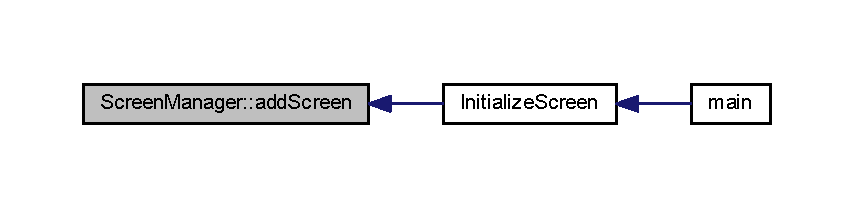
\includegraphics[width=350pt]{class_screen_manager_a2e6e206c2ff265c534c802898c9c078b_icgraph}
\end{center}
\end{figure}


\hypertarget{class_screen_manager_abcf990ad052121e6ebd2ab03771657df}{\index{Screen\-Manager@{Screen\-Manager}!Draw@{Draw}}
\index{Draw@{Draw}!ScreenManager@{Screen\-Manager}}
\subsubsection[{Draw}]{\setlength{\rightskip}{0pt plus 5cm}void Screen\-Manager\-::\-Draw (
\begin{DoxyParamCaption}
\item[{sf\-::\-Render\-Window \&}]{window, }
\item[{sf\-::\-Vector2f}]{offset}
\end{DoxyParamCaption}
)\hspace{0.3cm}{\ttfamily [virtual]}}}\label{class_screen_manager_abcf990ad052121e6ebd2ab03771657df}


Here is the call graph for this function\-:\nopagebreak
\begin{figure}[H]
\begin{center}
\leavevmode
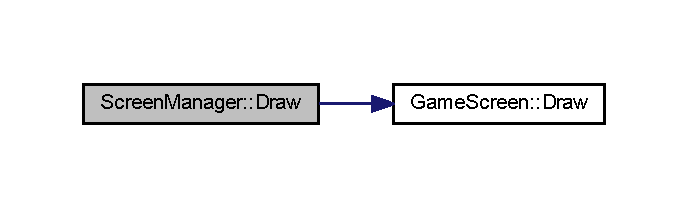
\includegraphics[width=330pt]{class_screen_manager_abcf990ad052121e6ebd2ab03771657df_cgraph}
\end{center}
\end{figure}




Here is the caller graph for this function\-:\nopagebreak
\begin{figure}[H]
\begin{center}
\leavevmode
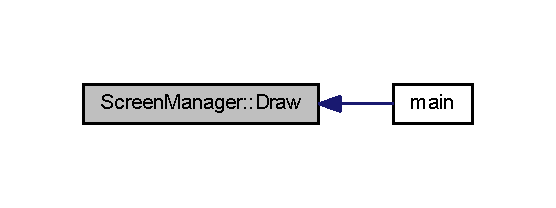
\includegraphics[width=267pt]{class_screen_manager_abcf990ad052121e6ebd2ab03771657df_icgraph}
\end{center}
\end{figure}


\hypertarget{class_screen_manager_a510ee04534746a6e72fa789539dc2d83}{\index{Screen\-Manager@{Screen\-Manager}!get\-Screen@{get\-Screen}}
\index{get\-Screen@{get\-Screen}!ScreenManager@{Screen\-Manager}}
\subsubsection[{get\-Screen}]{\setlength{\rightskip}{0pt plus 5cm}{\bf Game\-Screen}$\ast$ Screen\-Manager\-::get\-Screen (
\begin{DoxyParamCaption}
\item[{std\-::string}]{name}
\end{DoxyParamCaption}
)}}\label{class_screen_manager_a510ee04534746a6e72fa789539dc2d83}
\hypertarget{class_screen_manager_aa806de1587575859315d975daa025688}{\index{Screen\-Manager@{Screen\-Manager}!push\-Transaction@{push\-Transaction}}
\index{push\-Transaction@{push\-Transaction}!ScreenManager@{Screen\-Manager}}
\subsubsection[{push\-Transaction}]{\setlength{\rightskip}{0pt plus 5cm}void Screen\-Manager\-::push\-Transaction (
\begin{DoxyParamCaption}
\item[{{\bf Screen\-Transaction} $\ast$}]{transaction}
\end{DoxyParamCaption}
)}}\label{class_screen_manager_aa806de1587575859315d975daa025688}
\hypertarget{class_screen_manager_a9bb115d54e94b72618361f4a347e26c8}{\index{Screen\-Manager@{Screen\-Manager}!remove\-Screen@{remove\-Screen}}
\index{remove\-Screen@{remove\-Screen}!ScreenManager@{Screen\-Manager}}
\subsubsection[{remove\-Screen}]{\setlength{\rightskip}{0pt plus 5cm}void Screen\-Manager\-::remove\-Screen (
\begin{DoxyParamCaption}
\item[{std\-::string}]{name}
\end{DoxyParamCaption}
)}}\label{class_screen_manager_a9bb115d54e94b72618361f4a347e26c8}
\hypertarget{class_screen_manager_a578dea02971b86905fee58593622495b}{\index{Screen\-Manager@{Screen\-Manager}!set\-Active\-Screen@{set\-Active\-Screen}}
\index{set\-Active\-Screen@{set\-Active\-Screen}!ScreenManager@{Screen\-Manager}}
\subsubsection[{set\-Active\-Screen}]{\setlength{\rightskip}{0pt plus 5cm}void Screen\-Manager\-::set\-Active\-Screen (
\begin{DoxyParamCaption}
\item[{std\-::string}]{name}
\end{DoxyParamCaption}
)}}\label{class_screen_manager_a578dea02971b86905fee58593622495b}


Here is the caller graph for this function\-:\nopagebreak
\begin{figure}[H]
\begin{center}
\leavevmode
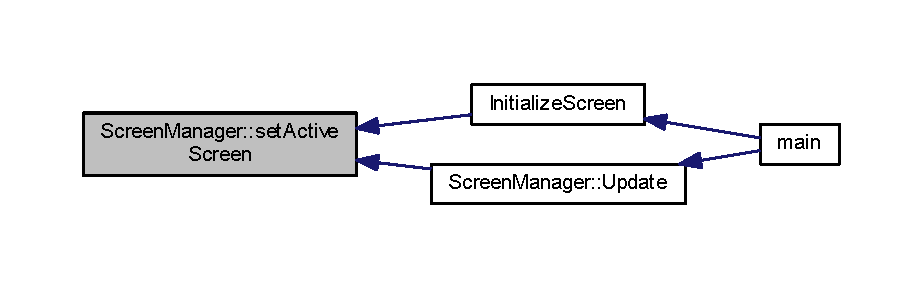
\includegraphics[width=350pt]{class_screen_manager_a578dea02971b86905fee58593622495b_icgraph}
\end{center}
\end{figure}


\hypertarget{class_screen_manager_a269d1b374ba195a036f03bd3caa897d9}{\index{Screen\-Manager@{Screen\-Manager}!Update@{Update}}
\index{Update@{Update}!ScreenManager@{Screen\-Manager}}
\subsubsection[{Update}]{\setlength{\rightskip}{0pt plus 5cm}void Screen\-Manager\-::\-Update (
\begin{DoxyParamCaption}
\item[{{\bf Update\-Data} $\ast$}]{updateobject}
\end{DoxyParamCaption}
)\hspace{0.3cm}{\ttfamily [virtual]}}}\label{class_screen_manager_a269d1b374ba195a036f03bd3caa897d9}


Here is the call graph for this function\-:\nopagebreak
\begin{figure}[H]
\begin{center}
\leavevmode
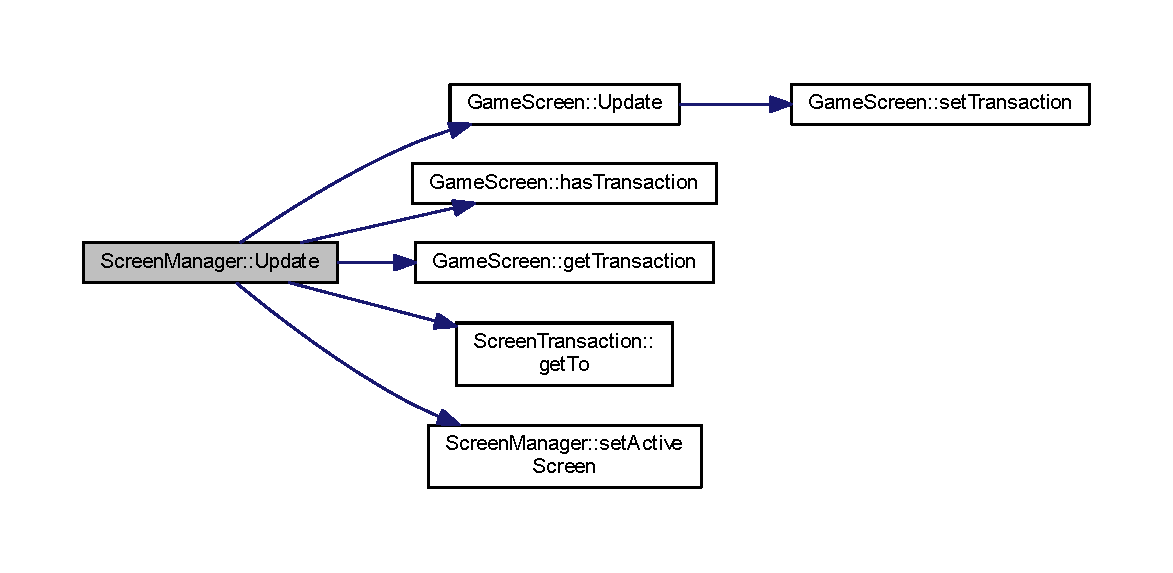
\includegraphics[width=350pt]{class_screen_manager_a269d1b374ba195a036f03bd3caa897d9_cgraph}
\end{center}
\end{figure}




Here is the caller graph for this function\-:\nopagebreak
\begin{figure}[H]
\begin{center}
\leavevmode
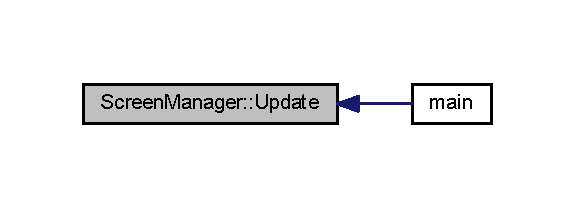
\includegraphics[width=276pt]{class_screen_manager_a269d1b374ba195a036f03bd3caa897d9_icgraph}
\end{center}
\end{figure}




\subsection{Member Data Documentation}
\hypertarget{class_screen_manager_abb46941be1b908a2b9d8053409e89597}{\index{Screen\-Manager@{Screen\-Manager}!Active\-Screen@{Active\-Screen}}
\index{Active\-Screen@{Active\-Screen}!ScreenManager@{Screen\-Manager}}
\subsubsection[{Active\-Screen}]{\setlength{\rightskip}{0pt plus 5cm}{\bf Game\-Screen}$\ast$ Screen\-Manager\-::\-Active\-Screen\hspace{0.3cm}{\ttfamily [private]}}}\label{class_screen_manager_abb46941be1b908a2b9d8053409e89597}
\hypertarget{class_screen_manager_a54eb2c9667efda525a35d0d7043e8807}{\index{Screen\-Manager@{Screen\-Manager}!Screens@{Screens}}
\index{Screens@{Screens}!ScreenManager@{Screen\-Manager}}
\subsubsection[{Screens}]{\setlength{\rightskip}{0pt plus 5cm}std\-::map$<$std\-::string, {\bf Game\-Screen} $\ast$$>$ Screen\-Manager\-::\-Screens\hspace{0.3cm}{\ttfamily [private]}}}\label{class_screen_manager_a54eb2c9667efda525a35d0d7043e8807}


The documentation for this class was generated from the following files\-:\begin{DoxyCompactItemize}
\item 
D\-:/\-Users/tom/\-Documents/\-Visual Studio 2013/\-Projects/\-Revelatorframework/\-Revelatorframework/\hyperlink{_screen_manager_8hpp}{Screen\-Manager.\-hpp}\item 
D\-:/\-Users/tom/\-Documents/\-Visual Studio 2013/\-Projects/\-Revelatorframework/\-Revelatorframework/\hyperlink{_screen_manager_8cpp}{Screen\-Manager.\-cpp}\end{DoxyCompactItemize}

\hypertarget{class_screen_transaction}{\section{Screen\-Transaction Class Reference}
\label{class_screen_transaction}\index{Screen\-Transaction@{Screen\-Transaction}}
}
\subsection*{Public Member Functions}
\begin{DoxyCompactItemize}
\item 
\hypertarget{class_screen_transaction_a5776ea6c2a6b7c7ec51744831e8e63b2}{{\bfseries Screen\-Transaction} (int id=0, std\-::string Message=\char`\"{}\char`\"{}, std\-::string from=\char`\"{}\char`\"{}, std\-::string to=\char`\"{}\char`\"{})}\label{class_screen_transaction_a5776ea6c2a6b7c7ec51744831e8e63b2}

\item 
\hypertarget{class_screen_transaction_a2fde50d60fd9dfefc3f93fdb9fadf0ae}{void {\bfseries set\-Message} (std\-::string mes)}\label{class_screen_transaction_a2fde50d60fd9dfefc3f93fdb9fadf0ae}

\item 
\hypertarget{class_screen_transaction_ae739629ae1f93e5754fc69f1d9ee96f7}{void {\bfseries set\-Id} (int id)}\label{class_screen_transaction_ae739629ae1f93e5754fc69f1d9ee96f7}

\item 
\hypertarget{class_screen_transaction_a5d652df4b9a696dbef724096b782b51e}{void {\bfseries set\-From} (std\-::string from)}\label{class_screen_transaction_a5d652df4b9a696dbef724096b782b51e}

\item 
\hypertarget{class_screen_transaction_aeb8dd00f22a18d66e36453c523fe9d83}{void {\bfseries set\-To} (std\-::string to)}\label{class_screen_transaction_aeb8dd00f22a18d66e36453c523fe9d83}

\item 
\hypertarget{class_screen_transaction_af012c8b10760e5ed7baf2c62846de590}{std\-::string {\bfseries get\-Message} ()}\label{class_screen_transaction_af012c8b10760e5ed7baf2c62846de590}

\item 
\hypertarget{class_screen_transaction_a7a788d3562c6ea040c1a4c0165fdc32a}{int {\bfseries get\-Id} ()}\label{class_screen_transaction_a7a788d3562c6ea040c1a4c0165fdc32a}

\item 
\hypertarget{class_screen_transaction_a6da0ff4e8c5f24c405c18331df6fe5ac}{std\-::string {\bfseries get\-From} ()}\label{class_screen_transaction_a6da0ff4e8c5f24c405c18331df6fe5ac}

\item 
\hypertarget{class_screen_transaction_a5348510109e53a87cb1233660c859e00}{std\-::string {\bfseries get\-To} ()}\label{class_screen_transaction_a5348510109e53a87cb1233660c859e00}

\end{DoxyCompactItemize}
\subsection*{Protected Attributes}
\begin{DoxyCompactItemize}
\item 
\hypertarget{class_screen_transaction_a212573d9bccda5210fb4bf82211fce07}{std\-::string {\bfseries Message}}\label{class_screen_transaction_a212573d9bccda5210fb4bf82211fce07}

\item 
\hypertarget{class_screen_transaction_acc2108d68c434499915514c1046d9806}{int {\bfseries Id}}\label{class_screen_transaction_acc2108d68c434499915514c1046d9806}

\item 
\hypertarget{class_screen_transaction_a6beff6473b1f9537a68feede691526e2}{std\-::string {\bfseries From}}\label{class_screen_transaction_a6beff6473b1f9537a68feede691526e2}

\item 
\hypertarget{class_screen_transaction_acadac834d980c73ac6084fb52a7f882c}{std\-::string {\bfseries To}}\label{class_screen_transaction_acadac834d980c73ac6084fb52a7f882c}

\end{DoxyCompactItemize}


The documentation for this class was generated from the following files\-:\begin{DoxyCompactItemize}
\item 
Revelatorfromework/Screen\-Transaction.\-hpp\item 
Revelatorfromework/Screen\-Transaction.\-cpp\end{DoxyCompactItemize}

\hypertarget{class_sensor}{\section{Sensor Class Reference}
\label{class_sensor}\index{Sensor@{Sensor}}
}


Inheritance diagram for Sensor\-:\nopagebreak
\begin{figure}[H]
\begin{center}
\leavevmode
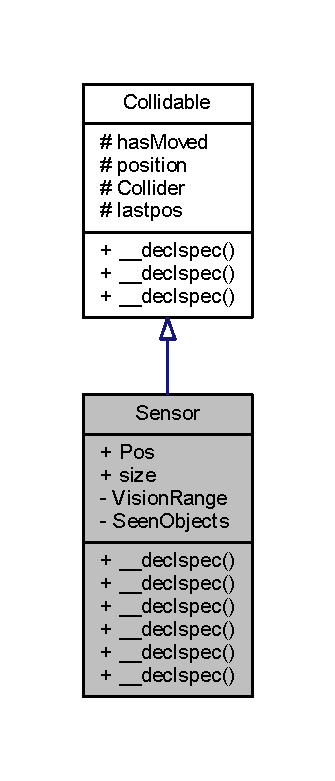
\includegraphics[width=139pt]{class_sensor__inherit__graph}
\end{center}
\end{figure}


Collaboration diagram for Sensor\-:\nopagebreak
\begin{figure}[H]
\begin{center}
\leavevmode
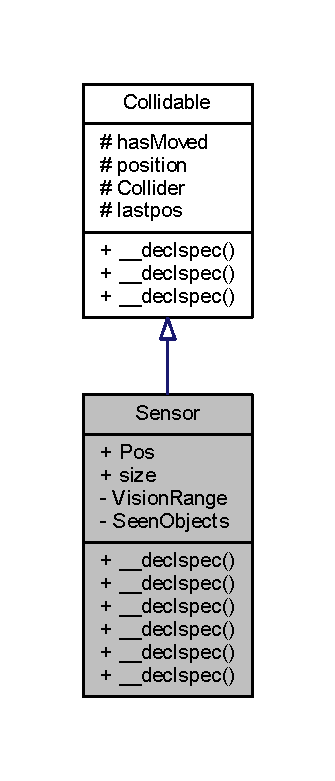
\includegraphics[width=166pt]{class_sensor__coll__graph}
\end{center}
\end{figure}
\subsection*{Public Member Functions}
\begin{DoxyCompactItemize}
\item 
\hypertarget{class_sensor_ac404bb7c1045796220e6d2997231feec}{{\bfseries Sensor} (float Radius, sf\-::\-Vector2f $\ast$Pos, sf\-::\-Vector2f size)}\label{class_sensor_ac404bb7c1045796220e6d2997231feec}

\item 
\hypertarget{class_sensor_a10dcb96d63d3991eff95b47f626d0e4c}{void {\bfseries add\-Seen\-Object} (\hyperlink{class_game_component}{Game\-Component} $\ast$comp)}\label{class_sensor_a10dcb96d63d3991eff95b47f626d0e4c}

\item 
\hypertarget{class_sensor_ac707ee7af9bd9adcdcb17d126582cc14}{\hyperlink{class_game_component}{Game\-Component} $\ast$ {\bfseries get\-Seen\-Object} ()}\label{class_sensor_ac707ee7af9bd9adcdcb17d126582cc14}

\item 
\hypertarget{class_sensor_ade01c8ff6de8daec5755b39bf4a57eae}{int {\bfseries Seen\-Object\-Count} ()}\label{class_sensor_ade01c8ff6de8daec5755b39bf4a57eae}

\item 
\hypertarget{class_sensor_ab7cc277606b8709a6df5fc53d7c0f22b}{float {\bfseries Get\-Vision\-Radius} ()}\label{class_sensor_ab7cc277606b8709a6df5fc53d7c0f22b}

\item 
\hypertarget{class_sensor_a8ed4309852c92cdeac0152cc2f604ac8}{void {\bfseries Draw\-Vision} (sf\-::\-Render\-Window \&window)}\label{class_sensor_a8ed4309852c92cdeac0152cc2f604ac8}

\end{DoxyCompactItemize}
\subsection*{Additional Inherited Members}


The documentation for this class was generated from the following files\-:\begin{DoxyCompactItemize}
\item 
Revelatorfromework/Sensor.\-hpp\item 
Revelatorfromework/Sensor.\-cpp\end{DoxyCompactItemize}

\hypertarget{class_spawner}{\section{Spawner Class Reference}
\label{class_spawner}\index{Spawner@{Spawner}}
}


{\ttfamily \#include $<$Spawner.\-hpp$>$}



Collaboration diagram for Spawner\-:\nopagebreak
\begin{figure}[H]
\begin{center}
\leavevmode
\includegraphics[width=161pt]{class_spawner__coll__graph}
\end{center}
\end{figure}
\subsection*{Public Member Functions}
\begin{DoxyCompactItemize}
\item 
\hyperlink{class_spawner_a2f9189658debef135e7ef3dae740dc60}{\-\_\-\-\_\-declspec} (dllexport) \hyperlink{class_spawner}{Spawner}()
\item 
\hyperlink{class_spawner_a7d9e09cf1588c58654650279268e02be}{\-\_\-\-\_\-declspec} (dllexport)$\sim$\hyperlink{class_spawner}{Spawner}()
\item 
\hyperlink{class_spawner_a3e3afb5a4121a7c2fa6f38950c88af31}{\-\_\-\-\_\-declspec} (dllexport) void push\-Component(\hyperlink{class_game_component}{Game\-Component} $\ast$c)
\item 
\hyperlink{class_spawner_aaf8e881a3933e8a582d2fe5d81abb9b1}{\-\_\-\-\_\-declspec} (dllexport) \hyperlink{class_game_component}{Game\-Component} $\ast$pop\-Component()
\item 
\hyperlink{class_spawner_a593f6964eae5b1d47bbc82701d2aa0df}{\-\_\-\-\_\-declspec} (dllexport) int Component\-Count()
\end{DoxyCompactItemize}
\subsection*{Private Attributes}
\begin{DoxyCompactItemize}
\item 
std\-::list$<$ \hyperlink{class_game_component}{Game\-Component} $\ast$ $>$ \hyperlink{class_spawner_ae5e316957ac1574347ba80bac3866976}{Components}
\end{DoxyCompactItemize}


\subsection{Member Function Documentation}
\hypertarget{class_spawner_a2f9189658debef135e7ef3dae740dc60}{\index{Spawner@{Spawner}!\-\_\-\-\_\-declspec@{\-\_\-\-\_\-declspec}}
\index{\-\_\-\-\_\-declspec@{\-\_\-\-\_\-declspec}!Spawner@{Spawner}}
\subsubsection[{\-\_\-\-\_\-declspec}]{\setlength{\rightskip}{0pt plus 5cm}Spawner\-::\-\_\-\-\_\-declspec (
\begin{DoxyParamCaption}
\item[{dllexport}]{}
\end{DoxyParamCaption}
)}}\label{class_spawner_a2f9189658debef135e7ef3dae740dc60}
\hypertarget{class_spawner_a7d9e09cf1588c58654650279268e02be}{\index{Spawner@{Spawner}!\-\_\-\-\_\-declspec@{\-\_\-\-\_\-declspec}}
\index{\-\_\-\-\_\-declspec@{\-\_\-\-\_\-declspec}!Spawner@{Spawner}}
\subsubsection[{\-\_\-\-\_\-declspec}]{\setlength{\rightskip}{0pt plus 5cm}Spawner\-::\-\_\-\-\_\-declspec (
\begin{DoxyParamCaption}
\item[{dllexport}]{}
\end{DoxyParamCaption}
)}}\label{class_spawner_a7d9e09cf1588c58654650279268e02be}
\hypertarget{class_spawner_a3e3afb5a4121a7c2fa6f38950c88af31}{\index{Spawner@{Spawner}!\-\_\-\-\_\-declspec@{\-\_\-\-\_\-declspec}}
\index{\-\_\-\-\_\-declspec@{\-\_\-\-\_\-declspec}!Spawner@{Spawner}}
\subsubsection[{\-\_\-\-\_\-declspec}]{\setlength{\rightskip}{0pt plus 5cm}Spawner\-::\-\_\-\-\_\-declspec (
\begin{DoxyParamCaption}
\item[{dllexport}]{}
\end{DoxyParamCaption}
)}}\label{class_spawner_a3e3afb5a4121a7c2fa6f38950c88af31}
\hypertarget{class_spawner_aaf8e881a3933e8a582d2fe5d81abb9b1}{\index{Spawner@{Spawner}!\-\_\-\-\_\-declspec@{\-\_\-\-\_\-declspec}}
\index{\-\_\-\-\_\-declspec@{\-\_\-\-\_\-declspec}!Spawner@{Spawner}}
\subsubsection[{\-\_\-\-\_\-declspec}]{\setlength{\rightskip}{0pt plus 5cm}Spawner\-::\-\_\-\-\_\-declspec (
\begin{DoxyParamCaption}
\item[{dllexport}]{}
\end{DoxyParamCaption}
)}}\label{class_spawner_aaf8e881a3933e8a582d2fe5d81abb9b1}
\hypertarget{class_spawner_a593f6964eae5b1d47bbc82701d2aa0df}{\index{Spawner@{Spawner}!\-\_\-\-\_\-declspec@{\-\_\-\-\_\-declspec}}
\index{\-\_\-\-\_\-declspec@{\-\_\-\-\_\-declspec}!Spawner@{Spawner}}
\subsubsection[{\-\_\-\-\_\-declspec}]{\setlength{\rightskip}{0pt plus 5cm}Spawner\-::\-\_\-\-\_\-declspec (
\begin{DoxyParamCaption}
\item[{dllexport}]{}
\end{DoxyParamCaption}
)}}\label{class_spawner_a593f6964eae5b1d47bbc82701d2aa0df}


\subsection{Member Data Documentation}
\hypertarget{class_spawner_ae5e316957ac1574347ba80bac3866976}{\index{Spawner@{Spawner}!Components@{Components}}
\index{Components@{Components}!Spawner@{Spawner}}
\subsubsection[{Components}]{\setlength{\rightskip}{0pt plus 5cm}std\-::list$<${\bf Game\-Component} $\ast$$>$ Spawner\-::\-Components\hspace{0.3cm}{\ttfamily [private]}}}\label{class_spawner_ae5e316957ac1574347ba80bac3866976}


The documentation for this class was generated from the following file\-:\begin{DoxyCompactItemize}
\item 
D\-:/\-Users/tom/\-Documents/\-Visual Studio 2013/\-Projects/\-Revelatorframework/\-Revelator\-Framework\-\_\-\-A\-P\-I/\hyperlink{_spawner_8hpp}{Spawner.\-hpp}\end{DoxyCompactItemize}

\hypertarget{class_update_data}{\section{Update\-Data Class Reference}
\label{class_update_data}\index{Update\-Data@{Update\-Data}}
}
\subsection*{Public Member Functions}
\begin{DoxyCompactItemize}
\item 
\hypertarget{class_update_data_a6882b130592cc63aa1e6f1ea36dcf349}{{\bfseries Update\-Data} (sf\-::\-Render\-Window $\ast$window)}\label{class_update_data_a6882b130592cc63aa1e6f1ea36dcf349}

\item 
\hypertarget{class_update_data_a2ff2fe51ef63293e7d4e831cc95b0837}{void {\bfseries Move\-Camera} (sf\-::\-Vector2f direction)}\label{class_update_data_a2ff2fe51ef63293e7d4e831cc95b0837}

\item 
\hypertarget{class_update_data_a17324f6ed80111443fef3da6208fb6bc}{void {\bfseries Set\-Camera\-Position} (sf\-::\-Vector2f Position)}\label{class_update_data_a17324f6ed80111443fef3da6208fb6bc}

\item 
\hypertarget{class_update_data_a81f654ff6f0879b2c3129662801232ec}{sf\-::\-Vector2f {\bfseries get\-Mouse\-Position} ()}\label{class_update_data_a81f654ff6f0879b2c3129662801232ec}

\item 
\hypertarget{class_update_data_a34912b36f314c985f9f725acae8bfb87}{bool {\bfseries get\-A} ()}\label{class_update_data_a34912b36f314c985f9f725acae8bfb87}

\item 
\hypertarget{class_update_data_a0485ded87f129d052690ba237b1e41dd}{bool {\bfseries get\-B} ()}\label{class_update_data_a0485ded87f129d052690ba237b1e41dd}

\item 
\hypertarget{class_update_data_a8a116007d883d35dbdb39eca6d22b80a}{bool {\bfseries get\-C} ()}\label{class_update_data_a8a116007d883d35dbdb39eca6d22b80a}

\item 
\hypertarget{class_update_data_aa9bebf60b7c0d589271abf0c7c5195f4}{bool {\bfseries get\-D} ()}\label{class_update_data_aa9bebf60b7c0d589271abf0c7c5195f4}

\item 
\hypertarget{class_update_data_aba4e9499df698ad2106d578e424bcdbd}{bool {\bfseries get\-E} ()}\label{class_update_data_aba4e9499df698ad2106d578e424bcdbd}

\item 
\hypertarget{class_update_data_a850bc599ed356ae2011fa2f1039799e8}{bool {\bfseries get\-F} ()}\label{class_update_data_a850bc599ed356ae2011fa2f1039799e8}

\item 
\hypertarget{class_update_data_ab9214503a879098cd82758290787358f}{bool {\bfseries get\-G} ()}\label{class_update_data_ab9214503a879098cd82758290787358f}

\item 
\hypertarget{class_update_data_abffec139846bbb6e399b95a714589036}{bool {\bfseries get\-H} ()}\label{class_update_data_abffec139846bbb6e399b95a714589036}

\item 
\hypertarget{class_update_data_ac2b180b0169806c7a28cc61eaf8c8524}{bool {\bfseries get\-I} ()}\label{class_update_data_ac2b180b0169806c7a28cc61eaf8c8524}

\item 
\hypertarget{class_update_data_a50376e12eaa0421bf9ddc45fb38c2f3e}{bool {\bfseries get\-J} ()}\label{class_update_data_a50376e12eaa0421bf9ddc45fb38c2f3e}

\item 
\hypertarget{class_update_data_a833401513efc900ea16ebbca9c6c376f}{bool {\bfseries get\-K} ()}\label{class_update_data_a833401513efc900ea16ebbca9c6c376f}

\item 
\hypertarget{class_update_data_a9fb4adb79c29ab471cd20e545369e461}{bool {\bfseries get\-L} ()}\label{class_update_data_a9fb4adb79c29ab471cd20e545369e461}

\item 
\hypertarget{class_update_data_a83eb14af87ca46cbf4efdcdf32c733f1}{bool {\bfseries get\-M} ()}\label{class_update_data_a83eb14af87ca46cbf4efdcdf32c733f1}

\item 
\hypertarget{class_update_data_ac1997d19b381268884e9567289f3b6ce}{bool {\bfseries get\-N} ()}\label{class_update_data_ac1997d19b381268884e9567289f3b6ce}

\item 
\hypertarget{class_update_data_a10f253930f0fcf19f9fe97605e78f29b}{bool {\bfseries get\-O} ()}\label{class_update_data_a10f253930f0fcf19f9fe97605e78f29b}

\item 
\hypertarget{class_update_data_a761422d59cc3d2c6c4e2ed03302c40ad}{bool {\bfseries get\-P} ()}\label{class_update_data_a761422d59cc3d2c6c4e2ed03302c40ad}

\item 
\hypertarget{class_update_data_a9eb538f77e90ec63fab15c8aa1b88d13}{bool {\bfseries get\-Q} ()}\label{class_update_data_a9eb538f77e90ec63fab15c8aa1b88d13}

\item 
\hypertarget{class_update_data_a521d053000d7ce7dbebe5e1a883b63ee}{bool {\bfseries get\-R} ()}\label{class_update_data_a521d053000d7ce7dbebe5e1a883b63ee}

\item 
\hypertarget{class_update_data_a9f461ba3436a319f3543ea8474c66a47}{bool {\bfseries get\-S} ()}\label{class_update_data_a9f461ba3436a319f3543ea8474c66a47}

\item 
\hypertarget{class_update_data_ac823fb26767e39fac95abce27edea53c}{bool {\bfseries get\-T} ()}\label{class_update_data_ac823fb26767e39fac95abce27edea53c}

\item 
\hypertarget{class_update_data_a7e816cd7d9962cfe204a0d9dd073794a}{bool {\bfseries get\-U} ()}\label{class_update_data_a7e816cd7d9962cfe204a0d9dd073794a}

\item 
\hypertarget{class_update_data_a412881a5ae5ea168046113f9287e65df}{bool {\bfseries get\-V} ()}\label{class_update_data_a412881a5ae5ea168046113f9287e65df}

\item 
\hypertarget{class_update_data_aff1ead12d71792ac878a09efd4aefb57}{bool {\bfseries get\-W} ()}\label{class_update_data_aff1ead12d71792ac878a09efd4aefb57}

\item 
\hypertarget{class_update_data_a98a5be607b3bd297ee74623ab656dd43}{bool {\bfseries get\-X} ()}\label{class_update_data_a98a5be607b3bd297ee74623ab656dd43}

\item 
\hypertarget{class_update_data_a97abbd1deaabc4bcdaf56f13e329cd65}{bool {\bfseries get\-Y} ()}\label{class_update_data_a97abbd1deaabc4bcdaf56f13e329cd65}

\item 
\hypertarget{class_update_data_a1b5e750c2954088111f27065470a70c7}{bool {\bfseries get\-Z} ()}\label{class_update_data_a1b5e750c2954088111f27065470a70c7}

\item 
\hypertarget{class_update_data_a3ccf74bec69653ac1d852955eec8a810}{bool {\bfseries get\-Num0} ()}\label{class_update_data_a3ccf74bec69653ac1d852955eec8a810}

\item 
\hypertarget{class_update_data_a8eda33976d01df351a385ec0dd2b7c35}{bool {\bfseries get\-Num1} ()}\label{class_update_data_a8eda33976d01df351a385ec0dd2b7c35}

\item 
\hypertarget{class_update_data_aef1ee75362623235d143c3307ac854fb}{bool {\bfseries get\-Num2} ()}\label{class_update_data_aef1ee75362623235d143c3307ac854fb}

\item 
\hypertarget{class_update_data_a3ccf64c3f32e0cb4d20405095aa81357}{bool {\bfseries get\-Num3} ()}\label{class_update_data_a3ccf64c3f32e0cb4d20405095aa81357}

\item 
\hypertarget{class_update_data_aba6d5e34064909fb9f64bf38d792c089}{bool {\bfseries get\-Num4} ()}\label{class_update_data_aba6d5e34064909fb9f64bf38d792c089}

\item 
\hypertarget{class_update_data_ae773ddb30244ad9f76d392a4bd5cbdae}{bool {\bfseries get\-Num5} ()}\label{class_update_data_ae773ddb30244ad9f76d392a4bd5cbdae}

\item 
\hypertarget{class_update_data_ad27b6d6989ce78c50ea48f328193d119}{bool {\bfseries get\-Num6} ()}\label{class_update_data_ad27b6d6989ce78c50ea48f328193d119}

\item 
\hypertarget{class_update_data_a2c9158bfbe33563923a6d3bf5190fe6c}{bool {\bfseries get\-Num7} ()}\label{class_update_data_a2c9158bfbe33563923a6d3bf5190fe6c}

\item 
\hypertarget{class_update_data_abc71c60234efc31e0e04d06d95315a8a}{bool {\bfseries get\-Num8} ()}\label{class_update_data_abc71c60234efc31e0e04d06d95315a8a}

\item 
\hypertarget{class_update_data_aee826ac50dcd4001c61f45b9000fdc6e}{bool {\bfseries get\-Num9} ()}\label{class_update_data_aee826ac50dcd4001c61f45b9000fdc6e}

\item 
\hypertarget{class_update_data_a846ba5bb9e86e12d4fb22845c9d5d705}{bool {\bfseries get\-Escape} ()}\label{class_update_data_a846ba5bb9e86e12d4fb22845c9d5d705}

\item 
\hypertarget{class_update_data_a879796f82489375ed0a31572590d336a}{bool {\bfseries get\-L\-Control} ()}\label{class_update_data_a879796f82489375ed0a31572590d336a}

\item 
\hypertarget{class_update_data_a85b0cd07aa88eaaecb740093f83e70ba}{bool {\bfseries get\-L\-Shift} ()}\label{class_update_data_a85b0cd07aa88eaaecb740093f83e70ba}

\item 
\hypertarget{class_update_data_abaf514ad59bc732b25daa0561c32100e}{bool {\bfseries get\-L\-Alt} ()}\label{class_update_data_abaf514ad59bc732b25daa0561c32100e}

\item 
\hypertarget{class_update_data_a38abae989d111f2c2c16f218fd9aad00}{bool {\bfseries get\-L\-System} ()}\label{class_update_data_a38abae989d111f2c2c16f218fd9aad00}

\item 
\hypertarget{class_update_data_a2984709c90638dec19ee40430f2154fb}{bool {\bfseries get\-R\-Control} ()}\label{class_update_data_a2984709c90638dec19ee40430f2154fb}

\item 
\hypertarget{class_update_data_a5d78d41fb8f4c3cf96fc9023c92b7f82}{bool {\bfseries get\-R\-Shift} ()}\label{class_update_data_a5d78d41fb8f4c3cf96fc9023c92b7f82}

\item 
\hypertarget{class_update_data_aec55065be384063726e953c84da37308}{bool {\bfseries get\-R\-Alt} ()}\label{class_update_data_aec55065be384063726e953c84da37308}

\item 
\hypertarget{class_update_data_a6b22f943435ce5668f32e3b0e7474081}{bool {\bfseries get\-R\-System} ()}\label{class_update_data_a6b22f943435ce5668f32e3b0e7474081}

\item 
\hypertarget{class_update_data_a719ab2ae19f40061e5c46847708b0113}{bool {\bfseries get\-Menu} ()}\label{class_update_data_a719ab2ae19f40061e5c46847708b0113}

\item 
\hypertarget{class_update_data_adaff4ef7db2f70afee4a0a1f6f5989fc}{bool {\bfseries get\-L\-Bracket} ()}\label{class_update_data_adaff4ef7db2f70afee4a0a1f6f5989fc}

\item 
\hypertarget{class_update_data_ae92d919c105c3672282b274dec47b31b}{bool {\bfseries get\-R\-Bracket} ()}\label{class_update_data_ae92d919c105c3672282b274dec47b31b}

\item 
\hypertarget{class_update_data_afeaa06e003e7f855db41443572c2697c}{bool {\bfseries get\-Semi\-Colon} ()}\label{class_update_data_afeaa06e003e7f855db41443572c2697c}

\item 
\hypertarget{class_update_data_a95690d070423256a8fac9f1c39395af3}{bool {\bfseries get\-Comma} ()}\label{class_update_data_a95690d070423256a8fac9f1c39395af3}

\item 
\hypertarget{class_update_data_aaf034236d4a5ab0e669a28bcf2c34a70}{bool {\bfseries get\-Period} ()}\label{class_update_data_aaf034236d4a5ab0e669a28bcf2c34a70}

\item 
\hypertarget{class_update_data_af4b426f024a3879c55c8ede49f62794a}{bool {\bfseries get\-Quote} ()}\label{class_update_data_af4b426f024a3879c55c8ede49f62794a}

\item 
\hypertarget{class_update_data_a1964067324c67d8a67eb5795df7e2106}{bool {\bfseries get\-Slash} ()}\label{class_update_data_a1964067324c67d8a67eb5795df7e2106}

\item 
\hypertarget{class_update_data_a061aba13ecec0d6bb57562ee0bf745cb}{bool {\bfseries get\-Back\-Slash} ()}\label{class_update_data_a061aba13ecec0d6bb57562ee0bf745cb}

\item 
\hypertarget{class_update_data_a107f1e0423fe1c6ef10736e5aaa73139}{bool {\bfseries get\-Tilde} ()}\label{class_update_data_a107f1e0423fe1c6ef10736e5aaa73139}

\item 
\hypertarget{class_update_data_a2ee6261586acff67a677a22a06915355}{bool {\bfseries get\-Equal} ()}\label{class_update_data_a2ee6261586acff67a677a22a06915355}

\item 
\hypertarget{class_update_data_a9eb4ec42e0c1e43ea26738b1045fb4bd}{bool {\bfseries get\-Dash} ()}\label{class_update_data_a9eb4ec42e0c1e43ea26738b1045fb4bd}

\item 
\hypertarget{class_update_data_a37643768c5a5c0c1344087cbfb7f9c4b}{bool {\bfseries get\-Space} ()}\label{class_update_data_a37643768c5a5c0c1344087cbfb7f9c4b}

\item 
\hypertarget{class_update_data_a2b4ecdaf41998df3072a931bddc5d98c}{bool {\bfseries get\-Return} ()}\label{class_update_data_a2b4ecdaf41998df3072a931bddc5d98c}

\item 
\hypertarget{class_update_data_a98e961e1f1dd9ac3d55595f1599d4b5c}{bool {\bfseries get\-Back\-Space} ()}\label{class_update_data_a98e961e1f1dd9ac3d55595f1599d4b5c}

\item 
\hypertarget{class_update_data_a0f504003d4e2b5bc6ecacace1d03b7b0}{bool {\bfseries get\-Tab} ()}\label{class_update_data_a0f504003d4e2b5bc6ecacace1d03b7b0}

\item 
\hypertarget{class_update_data_ad54388e377a99455abcd0e3b73c00c03}{bool {\bfseries get\-Page\-Up} ()}\label{class_update_data_ad54388e377a99455abcd0e3b73c00c03}

\item 
\hypertarget{class_update_data_a1074c3a9f2ad7f49602385e3c3123360}{bool {\bfseries get\-Page\-Down} ()}\label{class_update_data_a1074c3a9f2ad7f49602385e3c3123360}

\item 
\hypertarget{class_update_data_a2d85d14cb612dde8a99b45d50c31bbf4}{bool {\bfseries get\-End} ()}\label{class_update_data_a2d85d14cb612dde8a99b45d50c31bbf4}

\item 
\hypertarget{class_update_data_a4112e564ca3a7d01a65c1984431944bd}{bool {\bfseries get\-Home} ()}\label{class_update_data_a4112e564ca3a7d01a65c1984431944bd}

\item 
\hypertarget{class_update_data_a8b2a99c437be1674da5abb9961287374}{bool {\bfseries get\-Insert} ()}\label{class_update_data_a8b2a99c437be1674da5abb9961287374}

\item 
\hypertarget{class_update_data_a84816fde434b28fd9682a6089142dd01}{bool {\bfseries get\-Delete} ()}\label{class_update_data_a84816fde434b28fd9682a6089142dd01}

\item 
\hypertarget{class_update_data_a3e17439d9e09d1cee639300d540e4fa5}{bool {\bfseries get\-Add} ()}\label{class_update_data_a3e17439d9e09d1cee639300d540e4fa5}

\item 
\hypertarget{class_update_data_aa0f64dfb0841a6c9001bac694dd20184}{bool {\bfseries get\-Subtract} ()}\label{class_update_data_aa0f64dfb0841a6c9001bac694dd20184}

\item 
\hypertarget{class_update_data_aac430af808de21f96b13651973b9e0fe}{bool {\bfseries get\-Multiply} ()}\label{class_update_data_aac430af808de21f96b13651973b9e0fe}

\item 
\hypertarget{class_update_data_a291e35fbedf25986a393f38a596e566f}{bool {\bfseries get\-Divide} ()}\label{class_update_data_a291e35fbedf25986a393f38a596e566f}

\item 
\hypertarget{class_update_data_aa7e8fb2ee5945c4e75705e1bc66a506d}{bool {\bfseries get\-Left} ()}\label{class_update_data_aa7e8fb2ee5945c4e75705e1bc66a506d}

\item 
\hypertarget{class_update_data_a3b804ea9b4fff968cc58edc80fe19822}{bool {\bfseries get\-Right} ()}\label{class_update_data_a3b804ea9b4fff968cc58edc80fe19822}

\item 
\hypertarget{class_update_data_a3f429c27697b52944a1e6cb67e229c79}{bool {\bfseries get\-Up} ()}\label{class_update_data_a3f429c27697b52944a1e6cb67e229c79}

\item 
\hypertarget{class_update_data_a18e63ba0c088dce6e42a1530cba0866c}{bool {\bfseries get\-Down} ()}\label{class_update_data_a18e63ba0c088dce6e42a1530cba0866c}

\item 
\hypertarget{class_update_data_adde2ea0adf41dd5244cbf5fc6baa02e0}{bool {\bfseries get\-Numpad0} ()}\label{class_update_data_adde2ea0adf41dd5244cbf5fc6baa02e0}

\item 
\hypertarget{class_update_data_a6d2bedd924d8c6ee102a87208b525560}{bool {\bfseries get\-Numpad1} ()}\label{class_update_data_a6d2bedd924d8c6ee102a87208b525560}

\item 
\hypertarget{class_update_data_aa3cfec23376b6616ee9c7bce014c0ced}{bool {\bfseries get\-Numpad2} ()}\label{class_update_data_aa3cfec23376b6616ee9c7bce014c0ced}

\item 
\hypertarget{class_update_data_af357ea18de13653058336b6087a34742}{bool {\bfseries get\-Numpad3} ()}\label{class_update_data_af357ea18de13653058336b6087a34742}

\item 
\hypertarget{class_update_data_acd419da25bac466ac676fc474de4069f}{bool {\bfseries get\-Numpad4} ()}\label{class_update_data_acd419da25bac466ac676fc474de4069f}

\item 
\hypertarget{class_update_data_aee25b3ad9c6ff0871b96c61eea8f34ab}{bool {\bfseries get\-Numpad5} ()}\label{class_update_data_aee25b3ad9c6ff0871b96c61eea8f34ab}

\item 
\hypertarget{class_update_data_a8027eda0b719ce336d5a93d679a88cb7}{bool {\bfseries get\-Numpad6} ()}\label{class_update_data_a8027eda0b719ce336d5a93d679a88cb7}

\item 
\hypertarget{class_update_data_ae27d817ed25fc19a2c132fed35aa7f4e}{bool {\bfseries get\-Numpad7} ()}\label{class_update_data_ae27d817ed25fc19a2c132fed35aa7f4e}

\item 
\hypertarget{class_update_data_ad629272a0be7fc9281915d887a2b2a3e}{bool {\bfseries get\-Numpad8} ()}\label{class_update_data_ad629272a0be7fc9281915d887a2b2a3e}

\item 
\hypertarget{class_update_data_a2da627e8eb4d11d90faa8dfcca372725}{bool {\bfseries get\-Numpad9} ()}\label{class_update_data_a2da627e8eb4d11d90faa8dfcca372725}

\item 
\hypertarget{class_update_data_a468dc7fa0b12d41d4cda9708bc591b4c}{bool {\bfseries get\-F1} ()}\label{class_update_data_a468dc7fa0b12d41d4cda9708bc591b4c}

\item 
\hypertarget{class_update_data_adf04da55d7068aa73932b92e87cefe14}{bool {\bfseries get\-F2} ()}\label{class_update_data_adf04da55d7068aa73932b92e87cefe14}

\item 
\hypertarget{class_update_data_a23baa206949f21c3a92f2b0374d84d45}{bool {\bfseries get\-F3} ()}\label{class_update_data_a23baa206949f21c3a92f2b0374d84d45}

\item 
\hypertarget{class_update_data_a063f193eed70bbae3fde409ffdba3c2c}{bool {\bfseries get\-F4} ()}\label{class_update_data_a063f193eed70bbae3fde409ffdba3c2c}

\item 
\hypertarget{class_update_data_acf3d0efa012d835b48f2c8c4fdd58236}{bool {\bfseries get\-F5} ()}\label{class_update_data_acf3d0efa012d835b48f2c8c4fdd58236}

\item 
\hypertarget{class_update_data_a850a0cb09e6791935fa599a098a40da3}{bool {\bfseries get\-F6} ()}\label{class_update_data_a850a0cb09e6791935fa599a098a40da3}

\item 
\hypertarget{class_update_data_ae788e38de8821894a47f919b977e7e99}{bool {\bfseries get\-F7} ()}\label{class_update_data_ae788e38de8821894a47f919b977e7e99}

\item 
\hypertarget{class_update_data_af998602272cfaf1bff54a83eb8432fb2}{bool {\bfseries get\-F8} ()}\label{class_update_data_af998602272cfaf1bff54a83eb8432fb2}

\item 
\hypertarget{class_update_data_a49320803a615bffa3a12e9f09f71e58d}{bool {\bfseries get\-F9} ()}\label{class_update_data_a49320803a615bffa3a12e9f09f71e58d}

\item 
\hypertarget{class_update_data_aa97a34468f14a3838a24211dcb122d06}{bool {\bfseries get\-F10} ()}\label{class_update_data_aa97a34468f14a3838a24211dcb122d06}

\item 
\hypertarget{class_update_data_a247aa9ae1940b485e1f8a51412e9fa5d}{bool {\bfseries get\-F11} ()}\label{class_update_data_a247aa9ae1940b485e1f8a51412e9fa5d}

\item 
\hypertarget{class_update_data_a617b573c0d862f7084bba70b90a2e1b1}{bool {\bfseries get\-F12} ()}\label{class_update_data_a617b573c0d862f7084bba70b90a2e1b1}

\item 
\hypertarget{class_update_data_a247d97fa5db9173ed37b16b8eb505d3b}{bool {\bfseries get\-F13} ()}\label{class_update_data_a247d97fa5db9173ed37b16b8eb505d3b}

\item 
\hypertarget{class_update_data_a4030602c3d5ac1037ccea57c7c1a331b}{bool {\bfseries get\-F14} ()}\label{class_update_data_a4030602c3d5ac1037ccea57c7c1a331b}

\item 
\hypertarget{class_update_data_a094ad4398217aa38fd671a985fc60880}{bool {\bfseries get\-F15} ()}\label{class_update_data_a094ad4398217aa38fd671a985fc60880}

\item 
\hypertarget{class_update_data_a4ade0efcb105d66a6d573ddc6d044979}{bool {\bfseries get\-Pause} ()}\label{class_update_data_a4ade0efcb105d66a6d573ddc6d044979}

\item 
\hypertarget{class_update_data_a7505c6e459c53bbdb0812031e9a258c6}{bool {\bfseries get\-Mouse\-Left} ()}\label{class_update_data_a7505c6e459c53bbdb0812031e9a258c6}

\item 
\hypertarget{class_update_data_a226c48dacf9b5309640a1a25583115b6}{bool {\bfseries get\-Mouse\-Right} ()}\label{class_update_data_a226c48dacf9b5309640a1a25583115b6}

\item 
\hypertarget{class_update_data_ad35a1239212d0e498286ab0a4e9f14b0}{bool {\bfseries get\-Mouse\-Middle} ()}\label{class_update_data_ad35a1239212d0e498286ab0a4e9f14b0}

\item 
\hypertarget{class_update_data_a62a79016b1e473832d03ae46b89252ae}{bool {\bfseries get\-Mouse\-X\-Button1} ()}\label{class_update_data_a62a79016b1e473832d03ae46b89252ae}

\item 
\hypertarget{class_update_data_a3a72e28655b87878de8dafbf07b7d344}{bool {\bfseries get\-Mouse\-X\-Button2} ()}\label{class_update_data_a3a72e28655b87878de8dafbf07b7d344}

\end{DoxyCompactItemize}


The documentation for this class was generated from the following files\-:\begin{DoxyCompactItemize}
\item 
Revelatorfromework/Update\-Data.\-hpp\item 
Revelatorfromework/Update\-Data.\-cpp\end{DoxyCompactItemize}

\hypertarget{class_utils}{\section{Utils Class Reference}
\label{class_utils}\index{Utils@{Utils}}
}
\subsection*{Public Member Functions}
\begin{DoxyCompactItemize}
\item 
\hypertarget{class_utils_a1653aff7c075a5dd590d479d9b62242d}{{\bfseries Utils} (const \hyperlink{class_utils}{Utils} \&utils)=delete}\label{class_utils_a1653aff7c075a5dd590d479d9b62242d}

\item 
\hypertarget{class_utils_add93043cabc33d69f58b083f0e618849}{\hyperlink{class_utils}{Utils} \& {\bfseries operator=} (const \hyperlink{class_utils}{Utils} \&utils)=delete}\label{class_utils_add93043cabc33d69f58b083f0e618849}

\end{DoxyCompactItemize}
\subsection*{Static Public Member Functions}
\begin{DoxyCompactItemize}
\item 
\hypertarget{class_utils_ad50ce773764e9114decc8c415cd38d3e}{static \hyperlink{class_utils}{Utils} \& {\bfseries get\-Instance} ()}\label{class_utils_ad50ce773764e9114decc8c415cd38d3e}

\end{DoxyCompactItemize}


The documentation for this class was generated from the following files\-:\begin{DoxyCompactItemize}
\item 
Revelatorfromework/Utils.\-hpp\item 
Revelatorfromework/Utils.\-cpp\end{DoxyCompactItemize}

\hypertarget{class_window_manager}{\section{Window\-Manager Class Reference}
\label{class_window_manager}\index{Window\-Manager@{Window\-Manager}}
}


{\ttfamily \#include $<$Window\-Manager.\-hpp$>$}



Collaboration diagram for Window\-Manager\-:\nopagebreak
\begin{figure}[H]
\begin{center}
\leavevmode
\includegraphics[width=194pt]{class_window_manager__coll__graph}
\end{center}
\end{figure}
\subsection*{Public Member Functions}
\begin{DoxyCompactItemize}
\item 
\hyperlink{class_window_manager_a19fd6e41c42760af82460d9851780d82}{$\sim$\-Window\-Manager} ()
\item 
sf\-::\-Render\-Window $\ast$ \hyperlink{class_window_manager_a7051ab4ec34157357d2fc029b5283ba0}{get\-Window} ()
\item 
sf\-::\-Vector2f \hyperlink{class_window_manager_a6c6ca24d553fcbc205ca6eba14eea324}{get\-Camera\-Position} ()
\item 
void \hyperlink{class_window_manager_a5ee838ab6472ae7fcfd607831a8228d1}{set\-Camera\-Position} (sf\-::\-Vector2f position)
\item 
void \hyperlink{class_window_manager_abbc66e888f2a67ab0203357005bc89d8}{Move\-Camera} (sf\-::\-Vector2f direction)
\item 
void \hyperlink{class_window_manager_af570f14ac975aa3073a51238f5121d79}{Init\-Window} (sf\-::\-Video\-Mode video, std\-::string Name)
\item 
\hyperlink{class_window_manager_aff6aee52b2c1ab9fe85027262b4b877f}{Window\-Manager} (const \hyperlink{class_window_manager}{Window\-Manager} \&windowmanager)=delete
\item 
\hyperlink{class_window_manager}{Window\-Manager} \& \hyperlink{class_window_manager_a11afbf3f6296341434679bbedb44c989}{operator=} (const \hyperlink{class_window_manager}{Window\-Manager} \&windowmanager)=delete
\end{DoxyCompactItemize}
\subsection*{Static Public Member Functions}
\begin{DoxyCompactItemize}
\item 
static \hyperlink{class_window_manager}{Window\-Manager} \& \hyperlink{class_window_manager_a4f5e8cf13cbe4f2d80f3dbcf7f3fb2eb}{get\-Instance} ()
\end{DoxyCompactItemize}
\subsection*{Private Member Functions}
\begin{DoxyCompactItemize}
\item 
\hyperlink{class_window_manager_a3a283b34c19aaa20296befaabad4d29b}{Window\-Manager} ()
\end{DoxyCompactItemize}
\subsection*{Private Attributes}
\begin{DoxyCompactItemize}
\item 
sf\-::\-Render\-Window $\ast$ \hyperlink{class_window_manager_ac7ca38df4c12f4127e75939259ec108c}{window}
\item 
sf\-::\-Vector2f \hyperlink{class_window_manager_a459ad4d059f5c4f286c24af4550c6101}{Camera\-Position}
\end{DoxyCompactItemize}


\subsection{Constructor \& Destructor Documentation}
\hypertarget{class_window_manager_a19fd6e41c42760af82460d9851780d82}{\index{Window\-Manager@{Window\-Manager}!$\sim$\-Window\-Manager@{$\sim$\-Window\-Manager}}
\index{$\sim$\-Window\-Manager@{$\sim$\-Window\-Manager}!WindowManager@{Window\-Manager}}
\subsubsection[{$\sim$\-Window\-Manager}]{\setlength{\rightskip}{0pt plus 5cm}Window\-Manager\-::$\sim$\-Window\-Manager (
\begin{DoxyParamCaption}
{}
\end{DoxyParamCaption}
)}}\label{class_window_manager_a19fd6e41c42760af82460d9851780d82}
\hypertarget{class_window_manager_aff6aee52b2c1ab9fe85027262b4b877f}{\index{Window\-Manager@{Window\-Manager}!Window\-Manager@{Window\-Manager}}
\index{Window\-Manager@{Window\-Manager}!WindowManager@{Window\-Manager}}
\subsubsection[{Window\-Manager}]{\setlength{\rightskip}{0pt plus 5cm}Window\-Manager\-::\-Window\-Manager (
\begin{DoxyParamCaption}
\item[{const {\bf Window\-Manager} \&}]{windowmanager}
\end{DoxyParamCaption}
)\hspace{0.3cm}{\ttfamily [delete]}}}\label{class_window_manager_aff6aee52b2c1ab9fe85027262b4b877f}
\hypertarget{class_window_manager_a3a283b34c19aaa20296befaabad4d29b}{\index{Window\-Manager@{Window\-Manager}!Window\-Manager@{Window\-Manager}}
\index{Window\-Manager@{Window\-Manager}!WindowManager@{Window\-Manager}}
\subsubsection[{Window\-Manager}]{\setlength{\rightskip}{0pt plus 5cm}Window\-Manager\-::\-Window\-Manager (
\begin{DoxyParamCaption}
{}
\end{DoxyParamCaption}
)\hspace{0.3cm}{\ttfamily [private]}}}\label{class_window_manager_a3a283b34c19aaa20296befaabad4d29b}


\subsection{Member Function Documentation}
\hypertarget{class_window_manager_a6c6ca24d553fcbc205ca6eba14eea324}{\index{Window\-Manager@{Window\-Manager}!get\-Camera\-Position@{get\-Camera\-Position}}
\index{get\-Camera\-Position@{get\-Camera\-Position}!WindowManager@{Window\-Manager}}
\subsubsection[{get\-Camera\-Position}]{\setlength{\rightskip}{0pt plus 5cm}sf\-::\-Vector2f Window\-Manager\-::get\-Camera\-Position (
\begin{DoxyParamCaption}
{}
\end{DoxyParamCaption}
)}}\label{class_window_manager_a6c6ca24d553fcbc205ca6eba14eea324}


Here is the caller graph for this function\-:\nopagebreak
\begin{figure}[H]
\begin{center}
\leavevmode
\includegraphics[width=350pt]{class_window_manager_a6c6ca24d553fcbc205ca6eba14eea324_icgraph}
\end{center}
\end{figure}


\hypertarget{class_window_manager_a4f5e8cf13cbe4f2d80f3dbcf7f3fb2eb}{\index{Window\-Manager@{Window\-Manager}!get\-Instance@{get\-Instance}}
\index{get\-Instance@{get\-Instance}!WindowManager@{Window\-Manager}}
\subsubsection[{get\-Instance}]{\setlength{\rightskip}{0pt plus 5cm}{\bf Window\-Manager} \& Window\-Manager\-::get\-Instance (
\begin{DoxyParamCaption}
{}
\end{DoxyParamCaption}
)\hspace{0.3cm}{\ttfamily [static]}}}\label{class_window_manager_a4f5e8cf13cbe4f2d80f3dbcf7f3fb2eb}


Here is the caller graph for this function\-:\nopagebreak
\begin{figure}[H]
\begin{center}
\leavevmode
\includegraphics[width=350pt]{class_window_manager_a4f5e8cf13cbe4f2d80f3dbcf7f3fb2eb_icgraph}
\end{center}
\end{figure}


\hypertarget{class_window_manager_a7051ab4ec34157357d2fc029b5283ba0}{\index{Window\-Manager@{Window\-Manager}!get\-Window@{get\-Window}}
\index{get\-Window@{get\-Window}!WindowManager@{Window\-Manager}}
\subsubsection[{get\-Window}]{\setlength{\rightskip}{0pt plus 5cm}sf\-::\-Render\-Window $\ast$ Window\-Manager\-::get\-Window (
\begin{DoxyParamCaption}
{}
\end{DoxyParamCaption}
)}}\label{class_window_manager_a7051ab4ec34157357d2fc029b5283ba0}


Here is the caller graph for this function\-:\nopagebreak
\begin{figure}[H]
\begin{center}
\leavevmode
\includegraphics[width=350pt]{class_window_manager_a7051ab4ec34157357d2fc029b5283ba0_icgraph}
\end{center}
\end{figure}


\hypertarget{class_window_manager_af570f14ac975aa3073a51238f5121d79}{\index{Window\-Manager@{Window\-Manager}!Init\-Window@{Init\-Window}}
\index{Init\-Window@{Init\-Window}!WindowManager@{Window\-Manager}}
\subsubsection[{Init\-Window}]{\setlength{\rightskip}{0pt plus 5cm}void Window\-Manager\-::\-Init\-Window (
\begin{DoxyParamCaption}
\item[{sf\-::\-Video\-Mode}]{video, }
\item[{std\-::string}]{Name}
\end{DoxyParamCaption}
)}}\label{class_window_manager_af570f14ac975aa3073a51238f5121d79}


Here is the caller graph for this function\-:\nopagebreak
\begin{figure}[H]
\begin{center}
\leavevmode
\includegraphics[width=350pt]{class_window_manager_af570f14ac975aa3073a51238f5121d79_icgraph}
\end{center}
\end{figure}


\hypertarget{class_window_manager_abbc66e888f2a67ab0203357005bc89d8}{\index{Window\-Manager@{Window\-Manager}!Move\-Camera@{Move\-Camera}}
\index{Move\-Camera@{Move\-Camera}!WindowManager@{Window\-Manager}}
\subsubsection[{Move\-Camera}]{\setlength{\rightskip}{0pt plus 5cm}void Window\-Manager\-::\-Move\-Camera (
\begin{DoxyParamCaption}
\item[{sf\-::\-Vector2f}]{direction}
\end{DoxyParamCaption}
)}}\label{class_window_manager_abbc66e888f2a67ab0203357005bc89d8}


Here is the call graph for this function\-:\nopagebreak
\begin{figure}[H]
\begin{center}
\leavevmode
\includegraphics[width=350pt]{class_window_manager_abbc66e888f2a67ab0203357005bc89d8_cgraph}
\end{center}
\end{figure}


\hypertarget{class_window_manager_a11afbf3f6296341434679bbedb44c989}{\index{Window\-Manager@{Window\-Manager}!operator=@{operator=}}
\index{operator=@{operator=}!WindowManager@{Window\-Manager}}
\subsubsection[{operator=}]{\setlength{\rightskip}{0pt plus 5cm}{\bf Window\-Manager}\& Window\-Manager\-::operator= (
\begin{DoxyParamCaption}
\item[{const {\bf Window\-Manager} \&}]{windowmanager}
\end{DoxyParamCaption}
)\hspace{0.3cm}{\ttfamily [delete]}}}\label{class_window_manager_a11afbf3f6296341434679bbedb44c989}
\hypertarget{class_window_manager_a5ee838ab6472ae7fcfd607831a8228d1}{\index{Window\-Manager@{Window\-Manager}!set\-Camera\-Position@{set\-Camera\-Position}}
\index{set\-Camera\-Position@{set\-Camera\-Position}!WindowManager@{Window\-Manager}}
\subsubsection[{set\-Camera\-Position}]{\setlength{\rightskip}{0pt plus 5cm}void Window\-Manager\-::set\-Camera\-Position (
\begin{DoxyParamCaption}
\item[{sf\-::\-Vector2f}]{position}
\end{DoxyParamCaption}
)}}\label{class_window_manager_a5ee838ab6472ae7fcfd607831a8228d1}


Here is the caller graph for this function\-:\nopagebreak
\begin{figure}[H]
\begin{center}
\leavevmode
\includegraphics[width=350pt]{class_window_manager_a5ee838ab6472ae7fcfd607831a8228d1_icgraph}
\end{center}
\end{figure}




\subsection{Member Data Documentation}
\hypertarget{class_window_manager_a459ad4d059f5c4f286c24af4550c6101}{\index{Window\-Manager@{Window\-Manager}!Camera\-Position@{Camera\-Position}}
\index{Camera\-Position@{Camera\-Position}!WindowManager@{Window\-Manager}}
\subsubsection[{Camera\-Position}]{\setlength{\rightskip}{0pt plus 5cm}sf\-::\-Vector2f Window\-Manager\-::\-Camera\-Position\hspace{0.3cm}{\ttfamily [private]}}}\label{class_window_manager_a459ad4d059f5c4f286c24af4550c6101}
\hypertarget{class_window_manager_ac7ca38df4c12f4127e75939259ec108c}{\index{Window\-Manager@{Window\-Manager}!window@{window}}
\index{window@{window}!WindowManager@{Window\-Manager}}
\subsubsection[{window}]{\setlength{\rightskip}{0pt plus 5cm}sf\-::\-Render\-Window$\ast$ Window\-Manager\-::window\hspace{0.3cm}{\ttfamily [private]}}}\label{class_window_manager_ac7ca38df4c12f4127e75939259ec108c}


The documentation for this class was generated from the following files\-:\begin{DoxyCompactItemize}
\item 
D\-:/\-Users/tom/\-Documents/\-Visual Studio 2013/\-Projects/\-Revelatorframework/\-Revelator\-Framework\-\_\-\-A\-P\-I/\hyperlink{_window_manager_8hpp}{Window\-Manager.\-hpp}\item 
D\-:/\-Users/tom/\-Documents/\-Visual Studio 2013/\-Projects/\-Revelatorframework/\-Revelator\-Framework\-\_\-\-A\-P\-I/\hyperlink{_window_manager_8cpp}{Window\-Manager.\-cpp}\end{DoxyCompactItemize}

%--- End generated contents ---

% Index
\newpage
\phantomsection
\addcontentsline{toc}{chapter}{Index}
\printindex

\end{document}
